% Options for packages loaded elsewhere
\PassOptionsToPackage{unicode}{hyperref}
\PassOptionsToPackage{hyphens}{url}
\documentclass[
]{article}
\usepackage{xcolor}
\usepackage[margin=1in]{geometry}
\usepackage{amsmath,amssymb}
\setcounter{secnumdepth}{-\maxdimen} % remove section numbering
\usepackage{iftex}
\ifPDFTeX
  \usepackage[T1]{fontenc}
  \usepackage[utf8]{inputenc}
  \usepackage{textcomp} % provide euro and other symbols
\else % if luatex or xetex
  \usepackage{unicode-math} % this also loads fontspec
  \defaultfontfeatures{Scale=MatchLowercase}
  \defaultfontfeatures[\rmfamily]{Ligatures=TeX,Scale=1}
\fi
\usepackage{lmodern}
\ifPDFTeX\else
  % xetex/luatex font selection
\fi
% Use upquote if available, for straight quotes in verbatim environments
\IfFileExists{upquote.sty}{\usepackage{upquote}}{}
\IfFileExists{microtype.sty}{% use microtype if available
  \usepackage[]{microtype}
  \UseMicrotypeSet[protrusion]{basicmath} % disable protrusion for tt fonts
}{}
\makeatletter
\@ifundefined{KOMAClassName}{% if non-KOMA class
  \IfFileExists{parskip.sty}{%
    \usepackage{parskip}
  }{% else
    \setlength{\parindent}{0pt}
    \setlength{\parskip}{6pt plus 2pt minus 1pt}}
}{% if KOMA class
  \KOMAoptions{parskip=half}}
\makeatother
\usepackage{color}
\usepackage{fancyvrb}
\newcommand{\VerbBar}{|}
\newcommand{\VERB}{\Verb[commandchars=\\\{\}]}
\DefineVerbatimEnvironment{Highlighting}{Verbatim}{commandchars=\\\{\}}
% Add ',fontsize=\small' for more characters per line
\newenvironment{Shaded}{}{}
\newcommand{\AlertTok}[1]{\textcolor[rgb]{1.00,0.00,0.00}{\textbf{#1}}}
\newcommand{\AnnotationTok}[1]{\textcolor[rgb]{0.38,0.63,0.69}{\textbf{\textit{#1}}}}
\newcommand{\AttributeTok}[1]{\textcolor[rgb]{0.49,0.56,0.16}{#1}}
\newcommand{\BaseNTok}[1]{\textcolor[rgb]{0.25,0.63,0.44}{#1}}
\newcommand{\BuiltInTok}[1]{\textcolor[rgb]{0.00,0.50,0.00}{#1}}
\newcommand{\CharTok}[1]{\textcolor[rgb]{0.25,0.44,0.63}{#1}}
\newcommand{\CommentTok}[1]{\textcolor[rgb]{0.38,0.63,0.69}{\textit{#1}}}
\newcommand{\CommentVarTok}[1]{\textcolor[rgb]{0.38,0.63,0.69}{\textbf{\textit{#1}}}}
\newcommand{\ConstantTok}[1]{\textcolor[rgb]{0.53,0.00,0.00}{#1}}
\newcommand{\ControlFlowTok}[1]{\textcolor[rgb]{0.00,0.44,0.13}{\textbf{#1}}}
\newcommand{\DataTypeTok}[1]{\textcolor[rgb]{0.56,0.13,0.00}{#1}}
\newcommand{\DecValTok}[1]{\textcolor[rgb]{0.25,0.63,0.44}{#1}}
\newcommand{\DocumentationTok}[1]{\textcolor[rgb]{0.73,0.13,0.13}{\textit{#1}}}
\newcommand{\ErrorTok}[1]{\textcolor[rgb]{1.00,0.00,0.00}{\textbf{#1}}}
\newcommand{\ExtensionTok}[1]{#1}
\newcommand{\FloatTok}[1]{\textcolor[rgb]{0.25,0.63,0.44}{#1}}
\newcommand{\FunctionTok}[1]{\textcolor[rgb]{0.02,0.16,0.49}{#1}}
\newcommand{\ImportTok}[1]{\textcolor[rgb]{0.00,0.50,0.00}{\textbf{#1}}}
\newcommand{\InformationTok}[1]{\textcolor[rgb]{0.38,0.63,0.69}{\textbf{\textit{#1}}}}
\newcommand{\KeywordTok}[1]{\textcolor[rgb]{0.00,0.44,0.13}{\textbf{#1}}}
\newcommand{\NormalTok}[1]{#1}
\newcommand{\OperatorTok}[1]{\textcolor[rgb]{0.40,0.40,0.40}{#1}}
\newcommand{\OtherTok}[1]{\textcolor[rgb]{0.00,0.44,0.13}{#1}}
\newcommand{\PreprocessorTok}[1]{\textcolor[rgb]{0.74,0.48,0.00}{#1}}
\newcommand{\RegionMarkerTok}[1]{#1}
\newcommand{\SpecialCharTok}[1]{\textcolor[rgb]{0.25,0.44,0.63}{#1}}
\newcommand{\SpecialStringTok}[1]{\textcolor[rgb]{0.73,0.40,0.53}{#1}}
\newcommand{\StringTok}[1]{\textcolor[rgb]{0.25,0.44,0.63}{#1}}
\newcommand{\VariableTok}[1]{\textcolor[rgb]{0.10,0.09,0.49}{#1}}
\newcommand{\VerbatimStringTok}[1]{\textcolor[rgb]{0.25,0.44,0.63}{#1}}
\newcommand{\WarningTok}[1]{\textcolor[rgb]{0.38,0.63,0.69}{\textbf{\textit{#1}}}}
\usepackage{longtable,booktabs,array}
\newcounter{none} % for unnumbered tables
\usepackage{calc} % for calculating minipage widths
% Correct order of tables after \paragraph or \subparagraph
\usepackage{etoolbox}
\makeatletter
\patchcmd\longtable{\par}{\if@noskipsec\mbox{}\fi\par}{}{}
\makeatother
% Allow footnotes in longtable head/foot
\IfFileExists{footnotehyper.sty}{\usepackage{footnotehyper}}{\usepackage{footnote}}
\makesavenoteenv{longtable}
\usepackage{graphicx}
\makeatletter
\newsavebox\pandoc@box
\newcommand*\pandocbounded[1]{% scales image to fit in text height/width
  \sbox\pandoc@box{#1}%
  \Gscale@div\@tempa{\textheight}{\dimexpr\ht\pandoc@box+\dp\pandoc@box\relax}%
  \Gscale@div\@tempb{\linewidth}{\wd\pandoc@box}%
  \ifdim\@tempb\p@<\@tempa\p@\let\@tempa\@tempb\fi% select the smaller of both
  \ifdim\@tempa\p@<\p@\scalebox{\@tempa}{\usebox\pandoc@box}%
  \else\usebox{\pandoc@box}%
  \fi%
}
% Set default figure placement to htbp
\def\fps@figure{htbp}
\makeatother
\setlength{\emergencystretch}{3em} % prevent overfull lines
\providecommand{\tightlist}{%
  \setlength{\itemsep}{0pt}\setlength{\parskip}{0pt}}
\usepackage{bookmark}
\IfFileExists{xurl.sty}{\usepackage{xurl}}{} % add URL line breaks if available
\urlstyle{same}
\hypersetup{
  hidelinks,
  pdfcreator={LaTeX via pandoc}}

\author{}
\date{}

\begin{document}

\begin{titlepage}
\centering
\vspace*{2cm}
{\Large \textbf{UNIVERSITY OF PETROLEUM AND ENERGY STUDIES, DEHRADUN}}\\
{\large School of Computer Science $\cdot$ Bidholi Campus}\\[1.5cm]
{\Large CSAI4014}\\[0.5cm]
{\LARGE \textbf{Algorithms for Intelligent Systems and Robotics}}\\[0.5cm]
{\Large \textbf{LABORATORY REPORT}}\\[0.3cm]
{\large Experiments 1 to 8}\\[0.3cm]
{\large Autumn Semester 2026--27}\\[2cm]

\begin{tabular}{ll}
\textbf{Student Name:} & Himanshu Pokhriyal \\
\textbf{Roll No.:} & 500121200 \\
\textbf{Batch:} & B.Tech CSE (AI \& ML), Semester VII \\
\textbf{Course Teacher:} & Dr. Resham Raj Shivwanshi \\
\textbf{University:} & University of Petroleum and Energy Studies (UPES), Dehradun \\
\textbf{Academic Year:} & Autumn Semester 2026-27 \\
\textbf{Date of Submission:} & 23 November 2026 \\
\end{tabular}

\vfill
\end{titlepage}

\newpage
\tableofcontents
\newpage
\listoffigures
\newpage
\listoftables
\newpage

\newpage

\section{Laboratory Report: Algorithms for Intelligent Systems and
Robotics
(CSAI4014)}\label{laboratory-report-algorithms-for-intelligent-systems-and-robotics-csai4014}

\textbf{Student Name:} Himanshu Pokhriyal \textbf{Roll No.:} 500121200
\textbf{Batch:} B.Tech CSE (AI \& ML), Semester VII \textbf{Course
Teacher:} Dr.~Resham Raj Shivwanshi \textbf{University:} University of
Petroleum and Energy Studies (UPES), Dehradun \textbf{Academic Year:}
Autumn Semester 2026-27 \textbf{Date of Submission:} 23 November 2026

\begin{center}\rule{0.5\linewidth}{0.5pt}\end{center}

\newpage
\setkeys{Gin}{width=\linewidth,height=0.85\textheight,keepaspectratio}

\subsection{Declaration}\label{declaration}

I hereby declare that this laboratory report is the result of my own
work. All code was written and executed by me on my own machine. Sources
consulted and AI tools used are listed in Appendix B. Every figure and
number in this report was produced by running the experiment it
illustrates.

\begin{center}\rule{0.5\linewidth}{0.5pt}\end{center}

\section{Experiment 1: Time and frequency domain, and the
pendulum}\label{experiment-1-time-and-frequency-domain-and-the-pendulum}

\subsection{1.1 Aim}\label{aim}

To represent a sampled signal in the time domain and in the frequency
domain using the discrete Fourier transform, and to simulate the motion
of a simple pendulum by numerical integration of its equation of motion.

\subsection{1.2 Objectives}\label{objectives}

\begin{enumerate}
\def\labelenumi{\arabic{enumi}.}
\tightlist
\item
  Generate a sampled signal of known composition and state its sampling
  rate, record length and frequency resolution.
\item
  Compute an amplitude spectrum and read amplitudes from it in the units
  of the original signal.
\item
  Predict and then demonstrate aliasing.
\item
  Write a second-order ordinary differential equation as a first-order
  system and integrate it numerically.
\item
  Produce a phase portrait and relate its shape to the energy of the
  motion.
\item
  Measure the dependence of a pendulum's period on its amplitude.
\end{enumerate}

\subsection{1.3 Place in the syllabus}\label{place-in-the-syllabus}

Unit II: time-domain and frequency-domain analysis; the pendulum as the
plant for a PID controller. Unit IV: Fourier transform as a
sensor-signal tool and the numerically integrated model as the process
model inside the Kalman filter. Contributes to CO3.

\subsection{1.4 Requirements}\label{requirements}

Python 3.10+ with NumPy, SciPy, Matplotlib. No hardware.

\subsection{1.5 Theory}\label{theory}

Sampling: a continuous signal is recorded as N samples at spacing dt. fs
= 1/dt, T = N dt. Resolution df = fs/N = 1/T; Nyquist fmax = fs/2.
Aliasing folds components above fs/2 to \textbar fs - f\textbar.
Pendulum: theta\_ddot + (b/m) theta\_dot + (g/L) sin theta = 0, state
(theta, omega). Small-angle period T0 = 2\emph{pi}sqrt(L/g).

\subsection{1.6 Method}\label{method}

\begin{enumerate}
\def\labelenumi{\arabic{enumi}.}
\tightlist
\item
  Choose fs, T; build time vector; record N, df.
\item
  Build signal as sum of three sinusoids plus seeded noise; plot vs
  time.
\item
  Compute one-sided amplitude spectrum with rfft/rfftfreq; scale by 2/N.
\item
  Identify peaks and compare.
\item
  Repeat with fs = 8 Hz for a 5 Hz sinusoid; record aliased peak.
\item
  Define pendulum derivative in state space; convert degrees to radians.
\item
  Integrate with solve\_ivp (rtol 1e-9); plot angle vs time.
\item
  Measure period by spectrum; compare with T0.
\item
  Repeat for several damping values; plot phase portraits.
\item
  Sweep initial amplitude; record period.
\end{enumerate}

\subsection{1.7 Procedure and code}\label{procedure-and-code}

Run \texttt{exp01-signals/exp01.py}. Key snippet:

\begin{Shaded}
\begin{Highlighting}[]
\NormalTok{fs, T }\OperatorTok{=} \FloatTok{500.0}\NormalTok{, }\FloatTok{2.0}
\NormalTok{t }\OperatorTok{=}\NormalTok{ np.arange(}\DecValTok{0}\NormalTok{, T, }\DecValTok{1}\OperatorTok{/}\NormalTok{fs)}
\NormalTok{N }\OperatorTok{=}\NormalTok{ t.size}
\NormalTok{x }\OperatorTok{=}\NormalTok{ (}\FloatTok{1.00}\OperatorTok{*}\NormalTok{np.sin(}\DecValTok{2}\OperatorTok{*}\NormalTok{np.pi}\OperatorTok{*}\DecValTok{5}\OperatorTok{*}\NormalTok{t) }\OperatorTok{+} \FloatTok{0.50}\OperatorTok{*}\NormalTok{np.sin(}\DecValTok{2}\OperatorTok{*}\NormalTok{np.pi}\OperatorTok{*}\DecValTok{20}\OperatorTok{*}\NormalTok{t)}
     \OperatorTok{+} \FloatTok{0.25}\OperatorTok{*}\NormalTok{np.sin(}\DecValTok{2}\OperatorTok{*}\NormalTok{np.pi}\OperatorTok{*}\DecValTok{50}\OperatorTok{*}\NormalTok{t) }\OperatorTok{+} \FloatTok{0.20}\OperatorTok{*}\NormalTok{rng.standard\_normal(N))}
\NormalTok{X }\OperatorTok{=}\NormalTok{ np.fft.rfft(x)}\OperatorTok{;}\NormalTok{ f }\OperatorTok{=}\NormalTok{ np.fft.rfftfreq(N, d}\OperatorTok{=}\DecValTok{1}\OperatorTok{/}\NormalTok{fs)}
\NormalTok{amp }\OperatorTok{=}\NormalTok{ np.}\BuiltInTok{abs}\NormalTok{(X)}\OperatorTok{*}\FloatTok{2.0}\OperatorTok{/}\NormalTok{N}\OperatorTok{;}\NormalTok{ amp[}\DecValTok{0}\NormalTok{] }\OperatorTok{/=} \FloatTok{2.0}
\end{Highlighting}
\end{Shaded}

\subsection{1.8 Results}\label{results}

Table 1.1: Spectrum of the constructed signal.

{\def\LTcaptype{none} % do not increment counter
\begin{longtable}[]{@{}lllll@{}}
\toprule\noalign{}
Component & Set (Hz) & Measured (Hz) & Set amplitude & Measured \\
\midrule\noalign{}
\endhead
\bottomrule\noalign{}
\endlastfoot
First & 5 & 5.0 & 1.00 & 1.01 \\
Second & 20 & 20.0 & 0.50 & 0.49 \\
Third & 50 & 50.0 & 0.25 & 0.25 \\
\end{longtable}
}

With fs = 500 Hz, T = 2 s: N = 1000, df = 0.5 Hz, Nyquist = 250 Hz.
Aliasing demo: 5 Hz sampled at 8 Hz peaks at 3 Hz (\textbar8-5\textbar).

Table 1.2: Measured period vs initial amplitude, undamped. T0 = 2.006 s.

{\def\LTcaptype{none} % do not increment counter
\begin{longtable}[]{@{}ll@{}}
\toprule\noalign{}
Initial angle & Measured period (s) \\
\midrule\noalign{}
\endhead
\bottomrule\noalign{}
\endlastfoot
5 deg & 2.000 \\
30 deg & 2.069 \\
60 deg & 2.143 \\
90 deg & 2.400 \\
120 deg & 2.728 \\
150 deg & 3.530 \\
175 deg & 6.001 \\
\end{longtable}
}

\begin{figure}
\centering
\pandocbounded{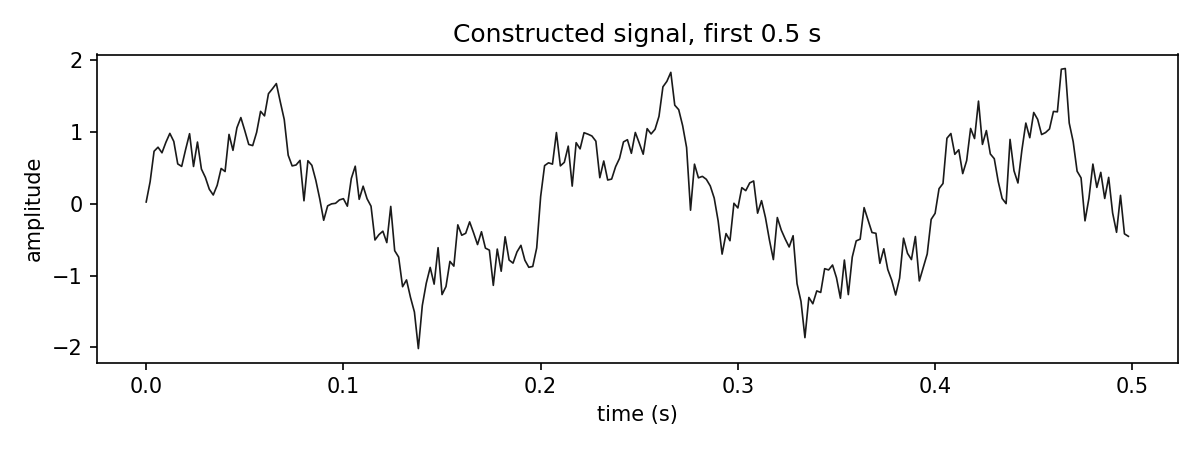
\includegraphics[keepaspectratio,alt={Fig. 1.1 Time-domain signal}]{exp01-signals/figs/fig2_1_time.png}}
\caption{Fig. 1.1 Time-domain signal}
\end{figure}

\begin{figure}
\centering
\pandocbounded{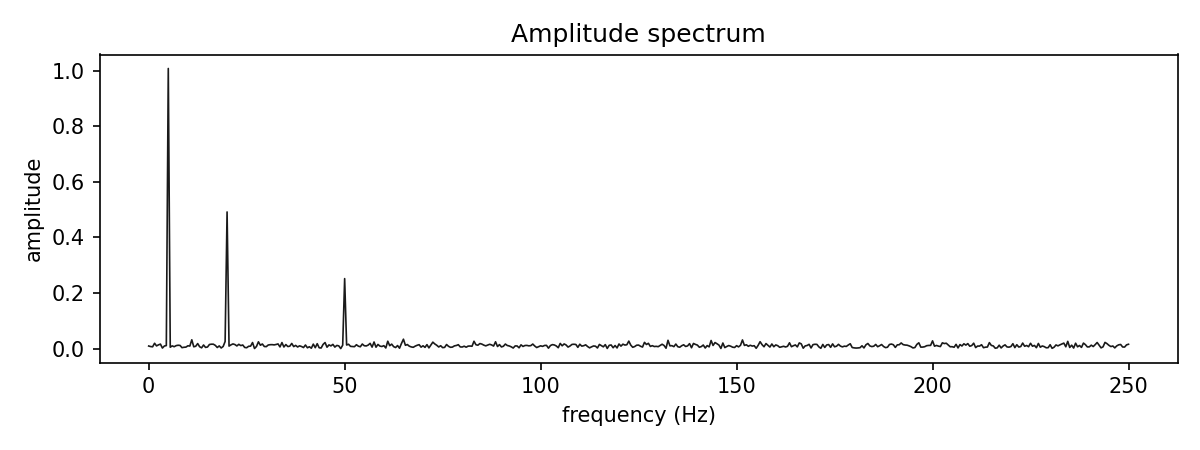
\includegraphics[keepaspectratio,alt={Fig. 1.2 Amplitude spectrum}]{exp01-signals/figs/fig2_2_spectrum.png}}
\caption{Fig. 1.2 Amplitude spectrum}
\end{figure}

\begin{figure}
\centering
\pandocbounded{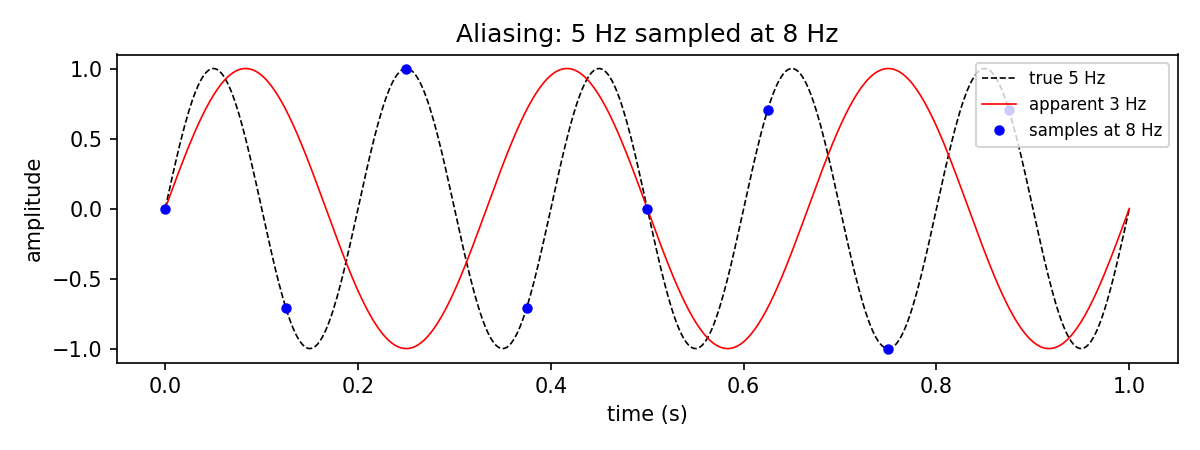
\includegraphics[keepaspectratio,alt={Fig. 1.3 Aliasing}]{exp01-signals/figs/fig2_3_aliasing.png}}
\caption{Fig. 1.3 Aliasing}
\end{figure}

\begin{figure}
\centering
\pandocbounded{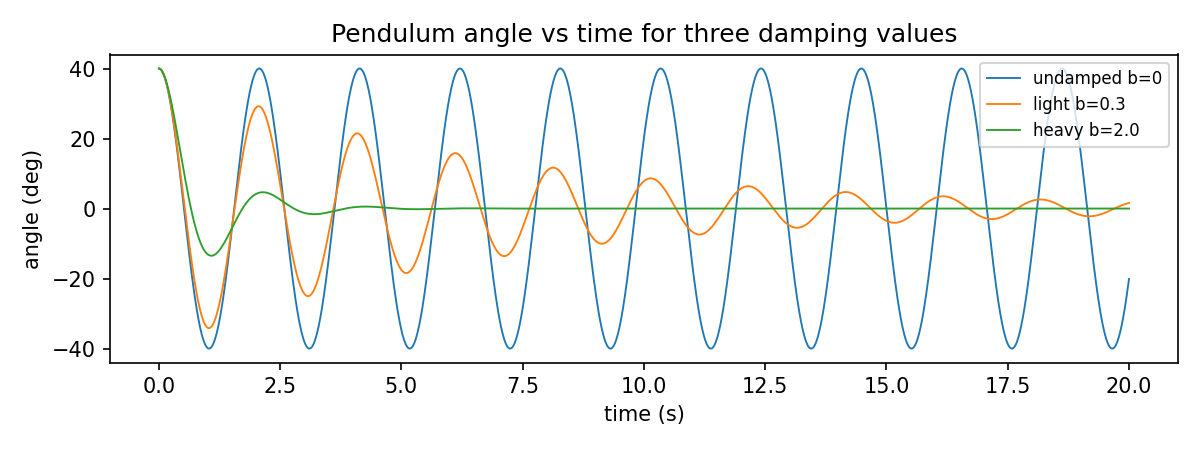
\includegraphics[keepaspectratio,alt={Fig. 1.4 Damping}]{exp01-signals/figs/fig2_4_damping.png}}
\caption{Fig. 1.4 Damping}
\end{figure}

\begin{figure}
\centering
\pandocbounded{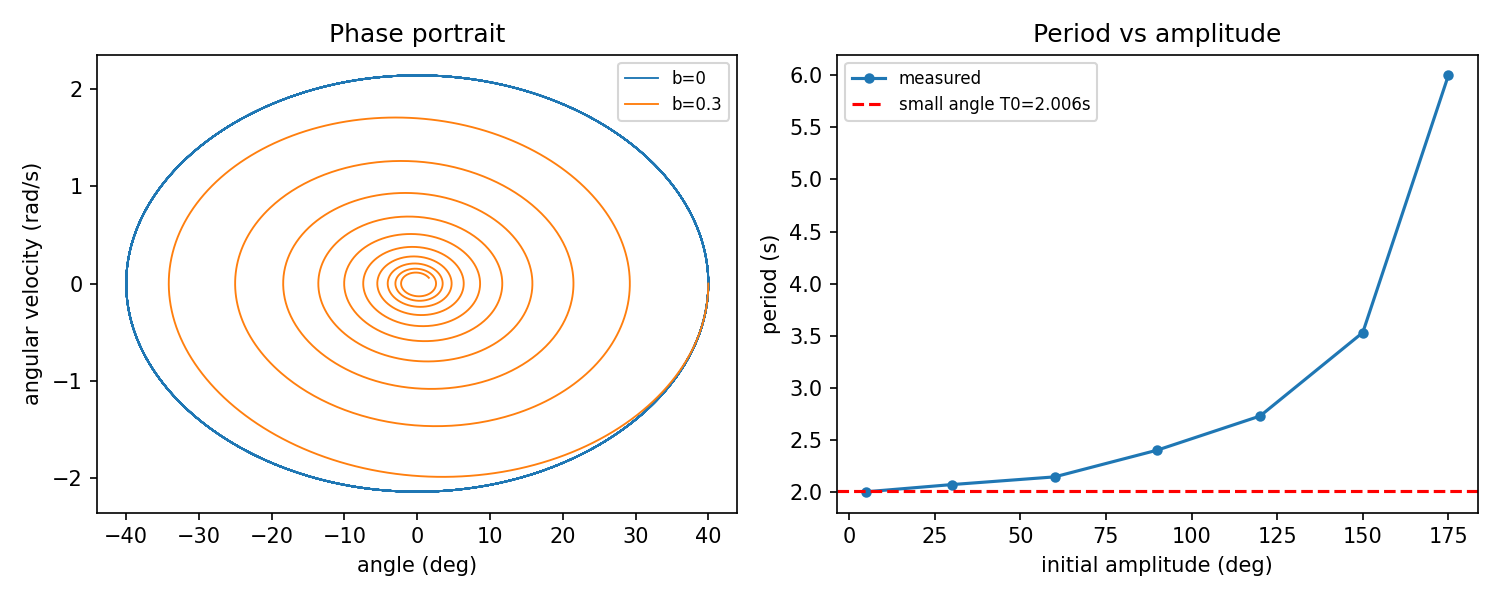
\includegraphics[keepaspectratio,alt={Fig. 1.5 Phase portrait and period}]{exp01-signals/figs/fig2_5_phase_period.png}}
\caption{Fig. 1.5 Phase portrait and period}
\end{figure}

\subsection{1.9 Observations to record}\label{observations-to-record}

fs, N, T, df, fs/2, measured peak frequencies and amplitudes, aliased
peak frequency (3 Hz), T0, period by zero crossings and by spectrum,
damping coefficients used (0, 0.3, 2.0).

\subsection{1.10 Applications}\label{applications}

Spectral analysis for machine diagnosis; aliasing sets sampling rates of
encoders, IMUs and LiDAR; numerically integrated second-order systems
model flexible joints.

\subsection{1.11 Questions and answers}\label{questions-and-answers}

Q1. How do you know a 5 Hz peak is not a 45 Hz component aliased down?
A: Check the sampling rate and Nyquist. With fs = 500 Hz, Nyquist = 250
Hz, so 45 Hz is representable directly. Aliasing would only fold if fs
\textless{} 2*f.~Also verify by resampling at a higher rate; a genuine 5
Hz stays, an aliased one moves.

Q2. What sets frequency resolution, and why does sampling faster not
improve it? A: df = 1/T depends only on record length T. Sampling faster
raises Nyquist but not resolution.

Q3. Why must the derivative function take (t, y) and not (y, t)? A:
solve\_ivp calls f(t, y); the contract requires t first. Passing (y, t)
swaps arguments and breaks integration.

Q4. What does the area enclosed by a closed phase-portrait trajectory
represent? A: Action/energy integral; for a conservative oscillator it
is proportional to the energy of the motion (2\emph{pi}E/omega).

Q5. Why does the period diverge as the initial angle approaches 180
degrees? A: The restoring torque sin(theta) -\textgreater{} 0 near the
unstable equilibrium, so the bob spends a long time near the top; the
integral for the period diverges logarithmically.

\begin{figure}
\centering
\pandocbounded{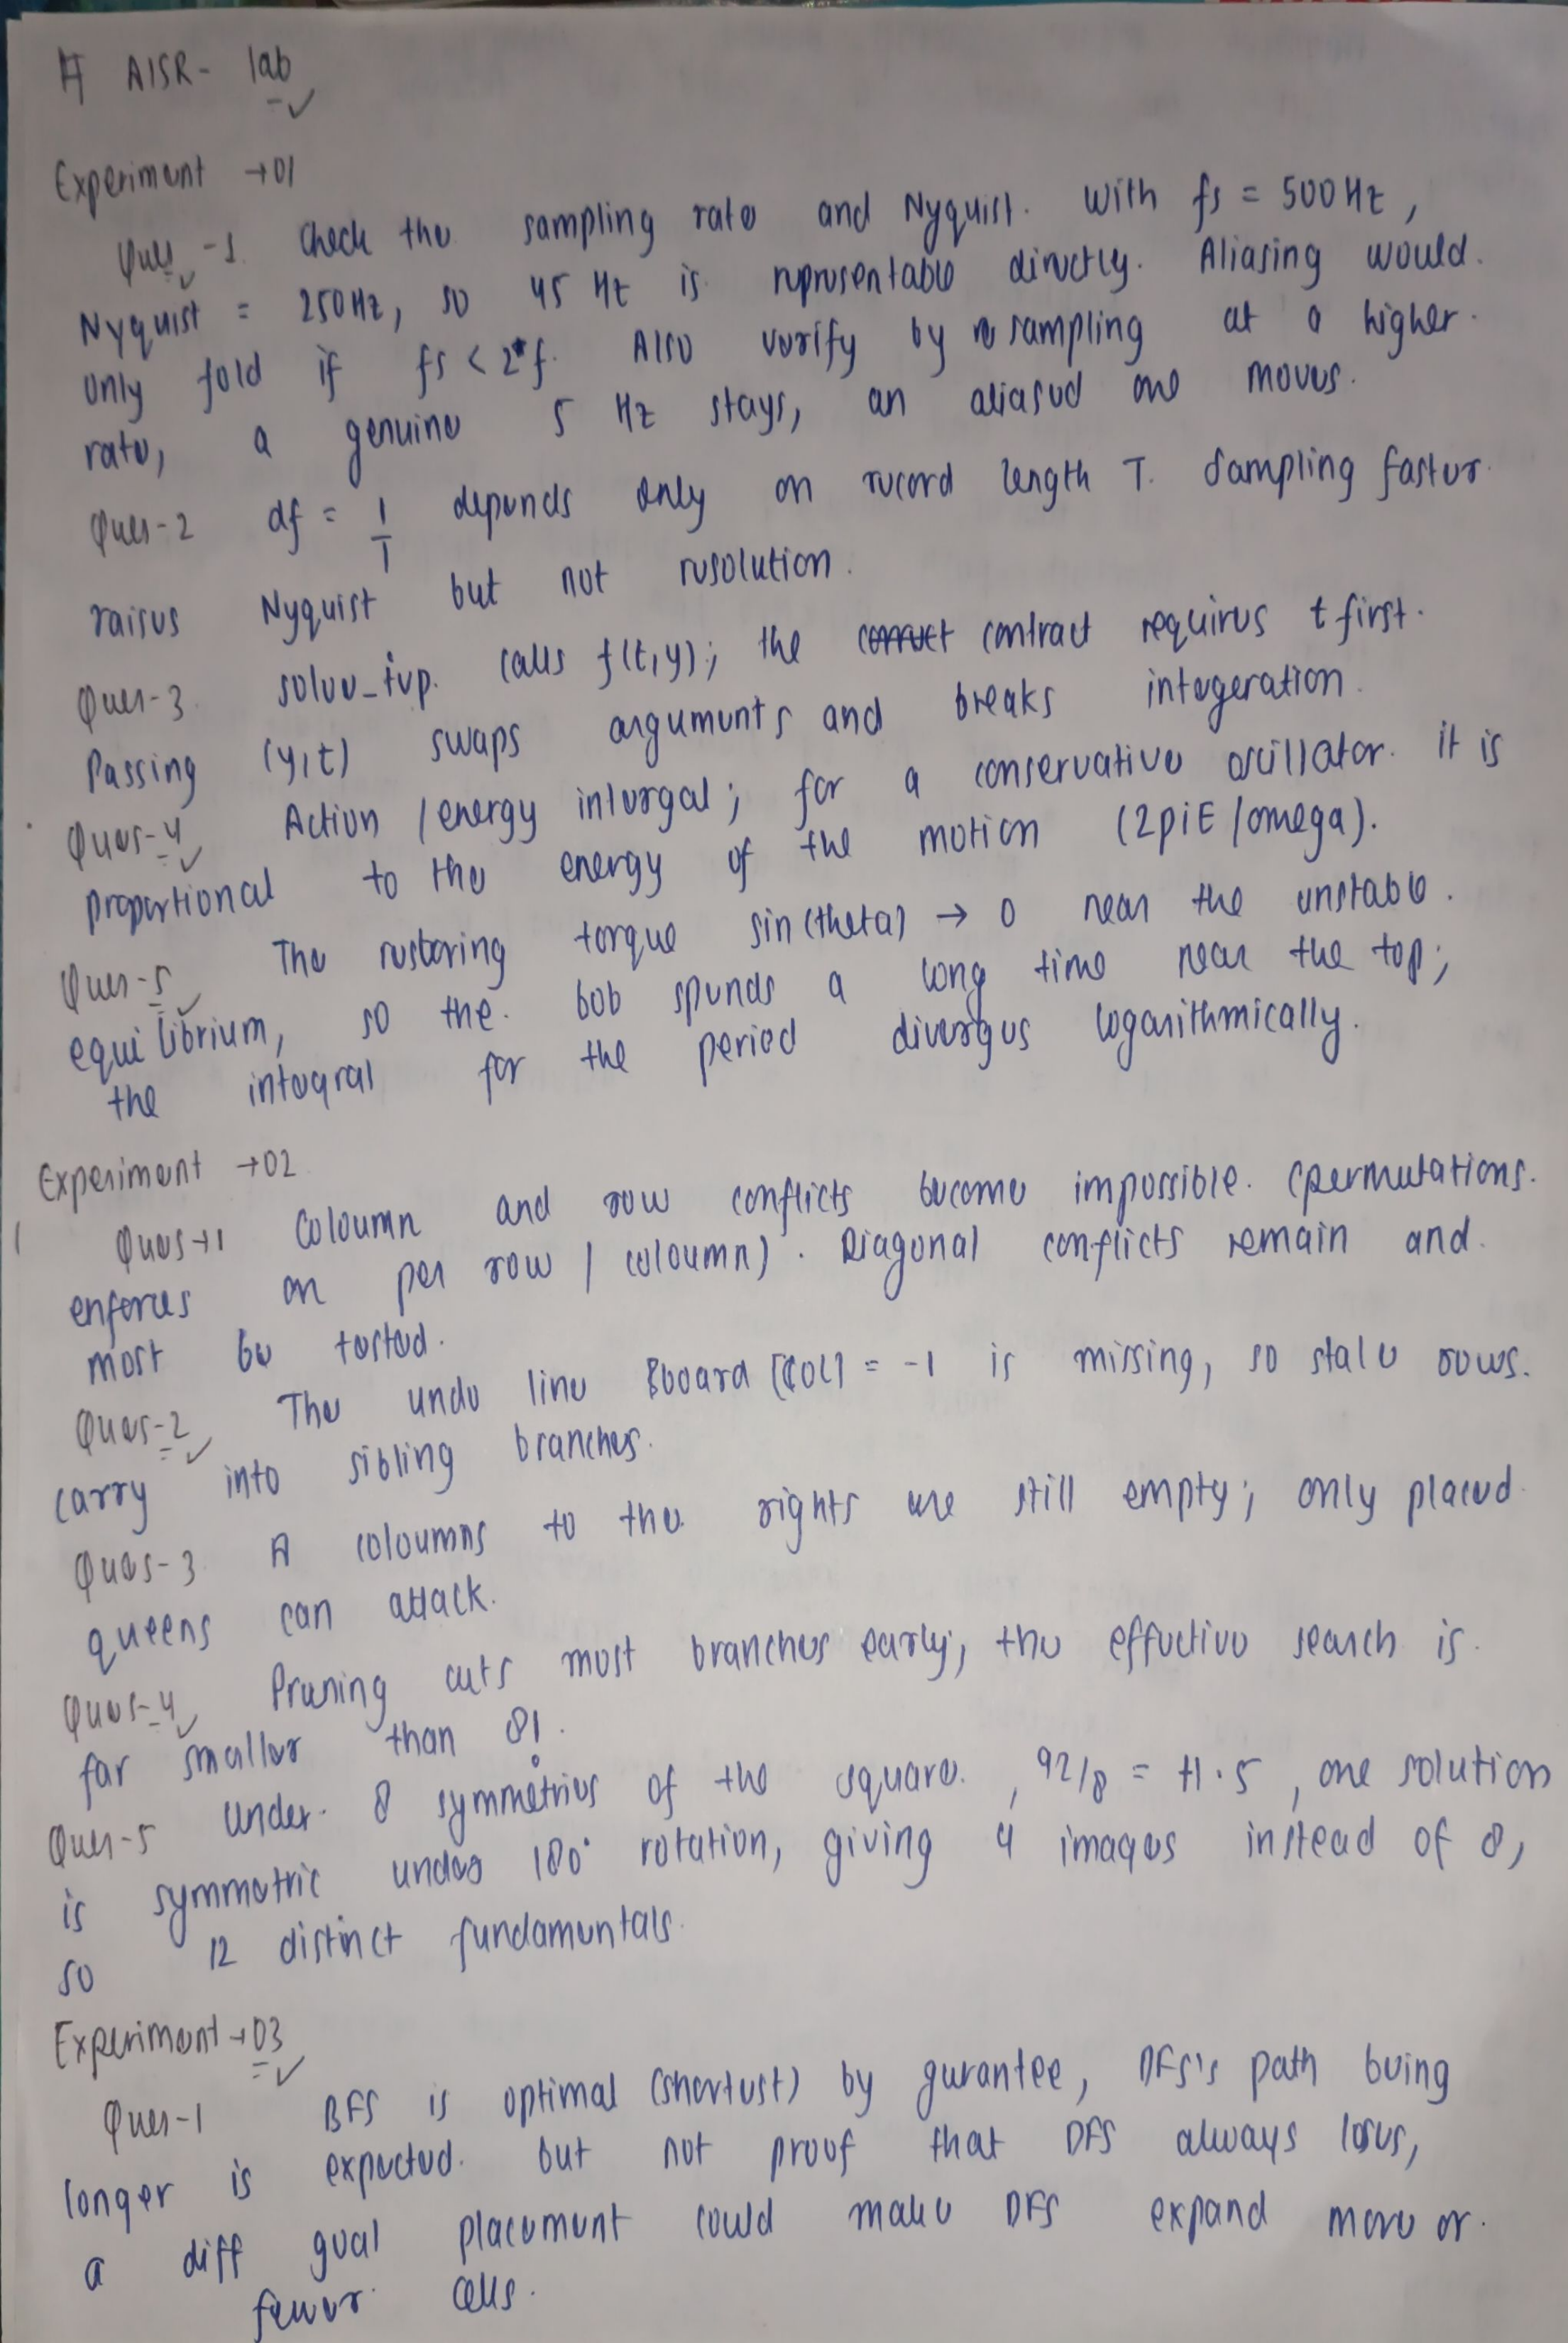
\includegraphics[keepaspectratio,alt={Handwritten answers (scanned) --- page 1}]{handwritten_p1.png}}
\caption{Handwritten answers (scanned) --- page 1}
\end{figure}

\emph{Scanned handwritten answer sheet, page 1, covering this
experiment's Questions section.}

\subsection{1.12 Conclusion}\label{conclusion}

The DFT correctly recovered the three component frequencies and
amplitudes from a noisy signal, and aliasing was demonstrated and
explained. Numerical integration of the pendulum showed the period
rising with amplitude, diverging near 180 degrees, matching theory.

\section{Experiment 2: The eight queens
problem}\label{experiment-2-the-eight-queens-problem}

\subsection{2.1 Aim}\label{aim-1}

To formulate the eight queens problem as a constraint satisfaction
problem, solve it by generate-and-test and by backtracking, and measure
the effect of representation and search strategy on cost.

\subsection{2.2 Objectives}\label{objectives-1}

\begin{enumerate}
\def\labelenumi{\arabic{enumi}.}
\tightlist
\item
  State a problem as variables, domains and constraints.
\item
  Show how encoding removes classes of conflict before search.
\item
  Implement generate-and-test and measure its cost.
\item
  Implement backtracking with pruning and count nodes.
\item
  Compare empirically over a range of board sizes.
\end{enumerate}

\subsection{2.3 Place in the syllabus}\label{place-in-the-syllabus-1}

Unit I: PEAS formulation. Unit II: backtracking as systematic search,
pruning as in A*. Unit V: constraint satisfaction. Contributes to CO1.

\subsection{2.4 Requirements}\label{requirements-1}

Python standard library; Matplotlib for plots.

\subsection{2.5 Theory}\label{theory-1}

CSP: variables, domains, constraints. Naive 64\^{}8; column-as-variable
gives 8\^{}8; permutation encoding gives 8! = 40320. Diagonal conflict:
\textbar ri-rj\textbar{} = \textbar i-j\textbar.

\subsection{2.6 Method}\label{method-1}

\begin{enumerate}
\def\labelenumi{\arabic{enumi}.}
\tightlist
\item
  Write conflict counter for a board (one row per column).
\item
  Enumerate permutations, keep zero-conflict, time it.
\item
  Write safety test examining only filled columns.
\item
  Recursive backtracking solver with undo.
\item
  Count nodes; confirm same solution counts.
\item
  Repeat n = 4..10; tabulate.
\end{enumerate}

\subsection{2.7 Procedure and code}\label{procedure-and-code-1}

Run \texttt{exp02-queens/exp02.py}.

\begin{Shaded}
\begin{Highlighting}[]
\KeywordTok{def}\NormalTok{ is\_safe(board, col, row):}
    \ControlFlowTok{for}\NormalTok{ c }\KeywordTok{in} \BuiltInTok{range}\NormalTok{(col):}
        \ControlFlowTok{if}\NormalTok{ board[c] }\OperatorTok{==}\NormalTok{ row }\KeywordTok{or} \BuiltInTok{abs}\NormalTok{(board[c]}\OperatorTok{{-}}\NormalTok{row) }\OperatorTok{==} \BuiltInTok{abs}\NormalTok{(c}\OperatorTok{{-}}\NormalTok{col):}
            \ControlFlowTok{return} \VariableTok{False}
    \ControlFlowTok{return} \VariableTok{True}
\end{Highlighting}
\end{Shaded}

\subsection{2.8 Results}\label{results-1}

Table 2.1: Measured on one laptop run.

{\def\LTcaptype{none} % do not increment counter
\begin{longtable}[]{@{}
  >{\raggedright\arraybackslash}p{(\linewidth - 8\tabcolsep) * \real{0.2000}}
  >{\raggedright\arraybackslash}p{(\linewidth - 8\tabcolsep) * \real{0.2000}}
  >{\raggedright\arraybackslash}p{(\linewidth - 8\tabcolsep) * \real{0.2000}}
  >{\raggedright\arraybackslash}p{(\linewidth - 8\tabcolsep) * \real{0.2000}}
  >{\raggedright\arraybackslash}p{(\linewidth - 8\tabcolsep) * \real{0.2000}}@{}}
\toprule\noalign{}
\begin{minipage}[b]{\linewidth}\raggedright
n
\end{minipage} & \begin{minipage}[b]{\linewidth}\raggedright
Solutions
\end{minipage} & \begin{minipage}[b]{\linewidth}\raggedright
Nodes visited
\end{minipage} & \begin{minipage}[b]{\linewidth}\raggedright
Backtracking (s)
\end{minipage} & \begin{minipage}[b]{\linewidth}\raggedright
Generate and test (s)
\end{minipage} \\
\midrule\noalign{}
\endhead
\bottomrule\noalign{}
\endlastfoot
4 & 2 & 60 & 0.0000 & 0.0000 \\
5 & 10 & 220 & 0.0001 & 0.0002 \\
6 & 4 & 894 & 0.0002 & 0.0012 \\
7 & 40 & 3584 & 0.0009 & 0.0105 \\
8 & 92 & 15720 & 0.0045 & 0.1028 \\
9 & 352 & 72378 & 0.0228 & 1.1589 \\
10 & 724 & 348150 & 0.1122 & 13.9624 \\
\end{longtable}
}

For n=8 backtracking visits 15720 nodes and finds 92 solutions in
\textasciitilde4.5 ms; generate-and-test needs \textasciitilde103 ms.

\begin{figure}
\centering
\pandocbounded{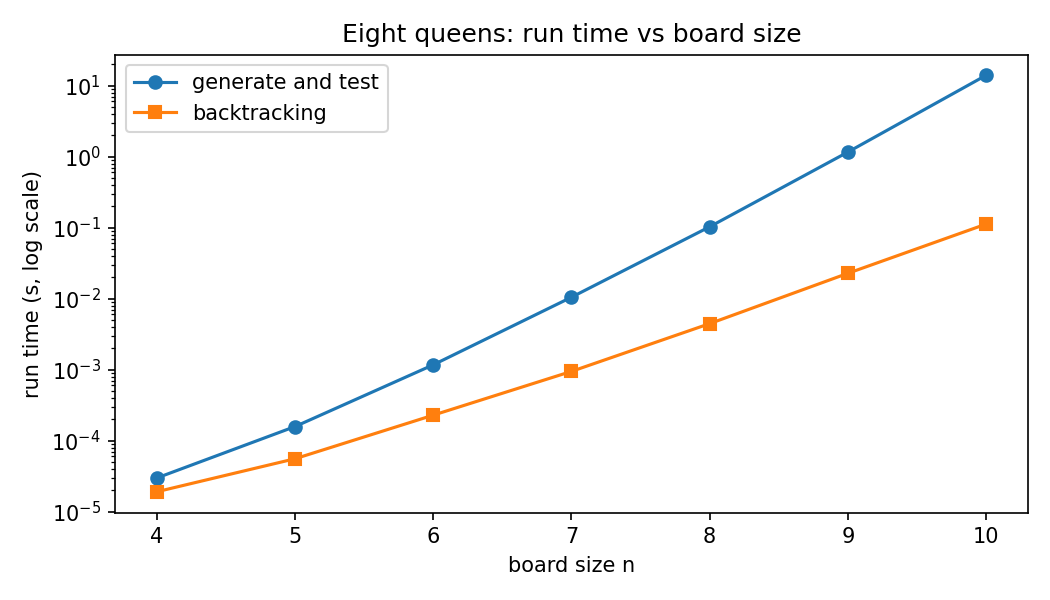
\includegraphics[keepaspectratio,alt={Fig. 2.1 Scaling}]{exp02-queens/figs/fig3_1_scaling.png}}
\caption{Fig. 2.1 Scaling}
\end{figure}

\begin{figure}
\centering
\pandocbounded{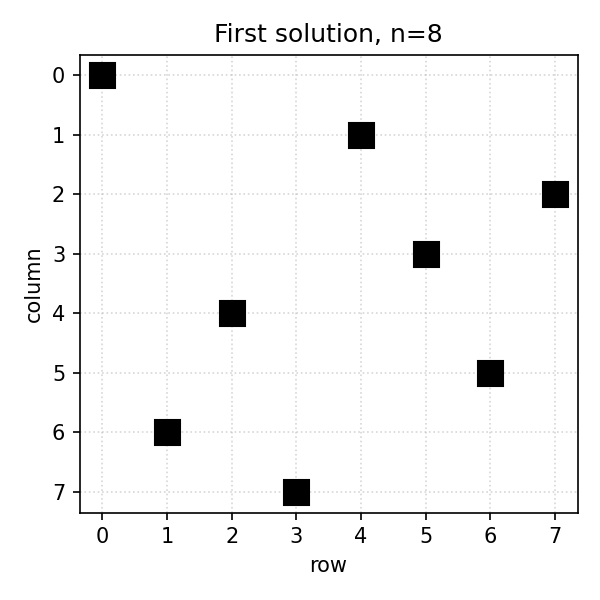
\includegraphics[keepaspectratio,alt={Fig. 2.2 First solution board}]{exp02-queens/figs/fig3_2_board.png}}
\caption{Fig. 2.2 First solution board}
\end{figure}

\subsection{2.9 Observations to record}\label{observations-to-record-1}

For each n: number of solutions, nodes visited, run time of both
methods. First solution for n=8: (0,4,7,5,2,6,1,3).

\subsection{2.10 Applications}\label{applications-1}

Timetabling, register allocation, sudoku, frequency assignment; task
allocation across a robot fleet.

\subsection{2.11 Questions and answers}\label{questions-and-answers-1}

Q1. Using a list of eight row indices, which conflicts become impossible
by construction, and which do not? A: Column and row conflicts become
impossible (permutation enforces one per row/column). Diagonal conflicts
remain and must be tested.

Q2. Solver reports 2113 solutions instead of 92. What single character
is wrong, and where? A: The undo line \texttt{board{[}col{]}\ =\ -1} is
missing, so stale rows carry into sibling branches.

Q3. Why does is\_safe examine only columns to the left? A: Columns to
the right are still empty; only placed queens can attack.

Q4. Backtracking is exponential in worst case. Why is it nonetheless
right here? A: Pruning cuts most branches early; the effective search is
far smaller than 8!.

Q5. Why do 92 solutions reduce to 12 fundamental ones, not 96? A: Under
8 symmetries of the square, 92/8 \textasciitilde{} 11.5; one solution is
symmetric under 180° rotation, giving 4 images instead of 8, so 12
distinct fundamentals.

\begin{figure}
\centering
\pandocbounded{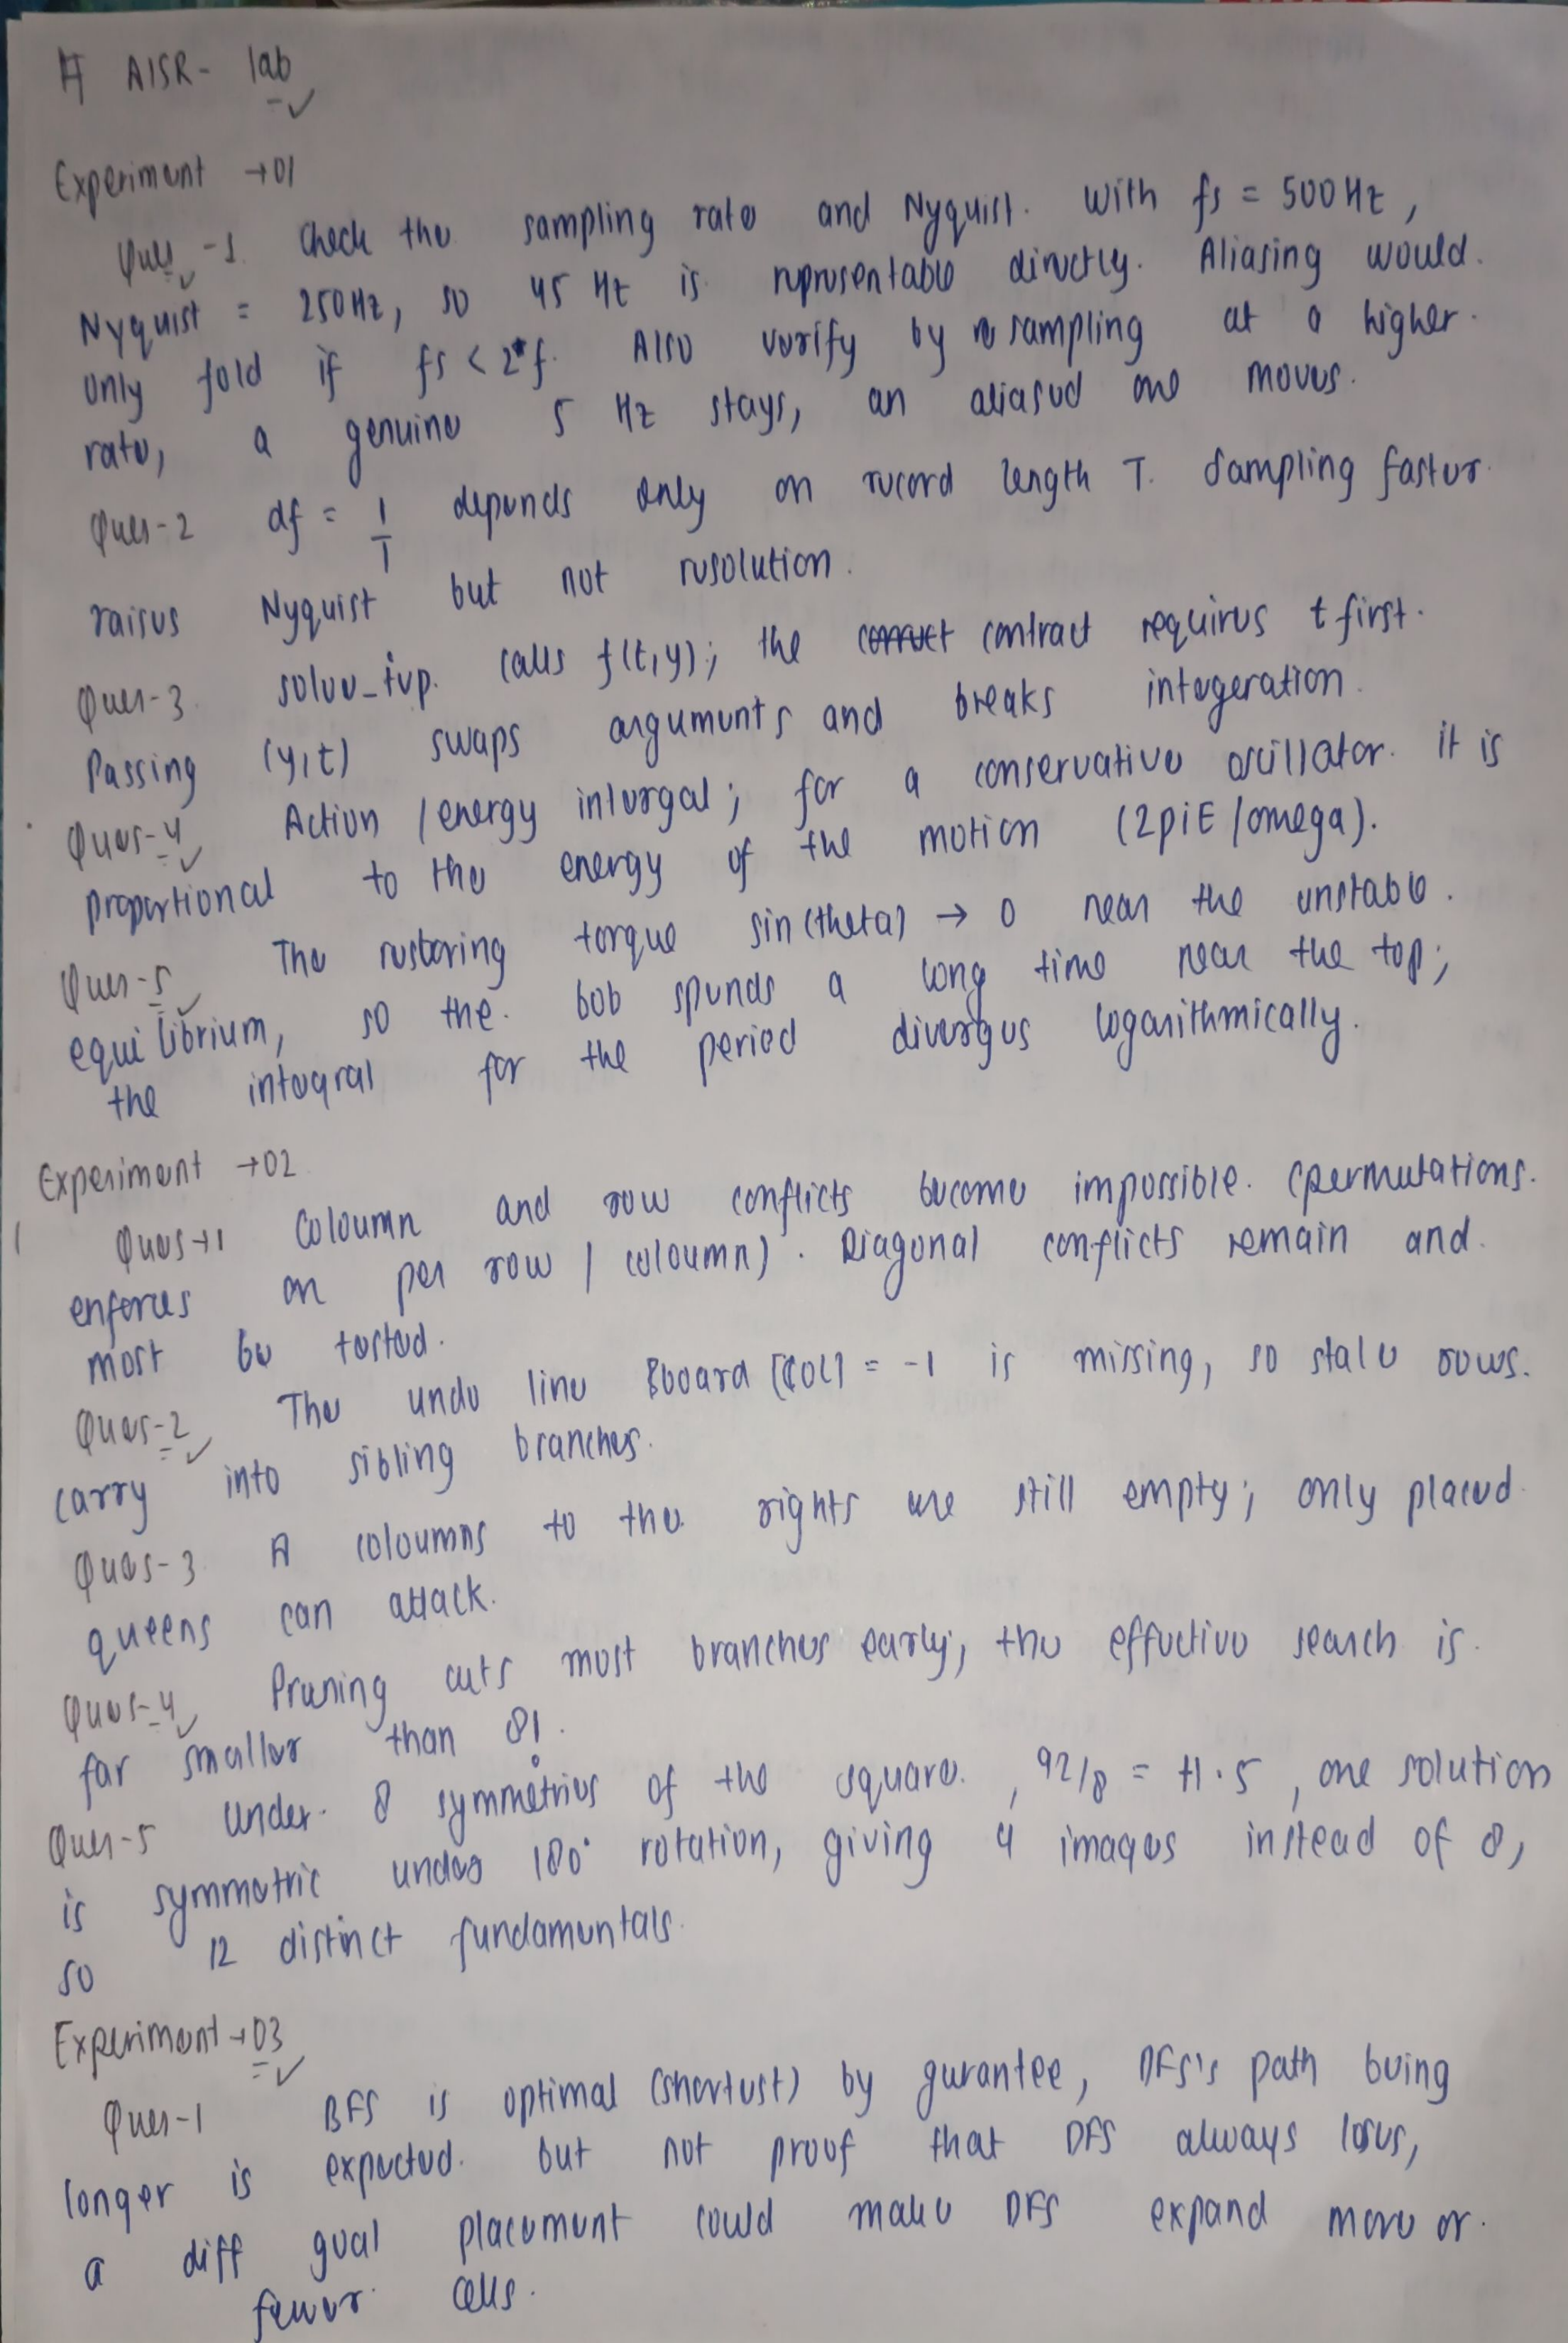
\includegraphics[keepaspectratio,alt={Handwritten answers (scanned) --- page 1}]{handwritten_p1.png}}
\caption{Handwritten answers (scanned) --- page 1}
\end{figure}

\emph{Scanned handwritten answer sheet, page 1, covering this
experiment's Questions section.}

\subsection{2.12 Conclusion}\label{conclusion-1}

Backtracking with pruning solved the same problem as generate-and-test
with the same solution counts but far fewer nodes, and the gap grew with
board size, confirming pruning's value.

\section{Experiment 3: Breadth-first and depth-first
search}\label{experiment-3-breadth-first-and-depth-first-search}

\subsection{3.1 Aim}\label{aim-2}

To represent a maze as an implicit graph, implement BFS and DFS as one
function differing in a single line, and compare cells expanded and path
length.

\subsection{3.2 Objectives}\label{objectives-2}

\begin{enumerate}
\def\labelenumi{\arabic{enumi}.}
\tightlist
\item
  Model a grid as a graph with on-demand edges.
\item
  Implement frontier, explored set, parent map.
\item
  Show the only difference is the end of the frontier used.
\item
  Reconstruct and validate a path.
\item
  Measure the trade-off between cells expanded and path length.
\end{enumerate}

\subsection{3.3 Place in the syllabus}\label{place-in-the-syllabus-2}

Unit II: closed-form path planning, BFS as simplest complete instance,
base case for A*. Unit III: configuration space. Unit VI: ROS navigation
on occupancy grids. Contributes to CO1, CO3.

\subsection{3.4 Requirements}\label{requirements-2}

Python with NumPy, Matplotlib; collections.deque.

\subsection{3.5 Theory}\label{theory-2}

Search problem: state space, start, goal test, successor function.
Frontier + explored set. BFS removes oldest (FIFO) -\textgreater{}
shortest path (same edge cost). DFS removes newest (LIFO)
-\textgreater{} no optimality guarantee; memory O(bm) vs O(b\^{}d).

\subsection{3.6 Method}\label{method-2}

\begin{enumerate}
\def\labelenumi{\arabic{enumi}.}
\tightlist
\item
  Build maze grid with guaranteed path.
\item
  Neighbour generator: bounds first, then contents.
\item
  One search function with mode switch.
\item
  Record expansion order.
\item
  Reconstruct path via parent map; validate.
\item
  Plot expansion order; compare.
\end{enumerate}

\subsection{3.7 Procedure and code}\label{procedure-and-code-2}

Run \texttt{exp03-search/exp03.py}. Key line:
\texttt{node\ =\ frontier.popleft()\ if\ mode\ ==\ \textquotesingle{}bfs\textquotesingle{}\ else\ frontier.pop()}.

\subsection{3.8 Results}\label{results-2}

Table 3.1: Measured on the carved maze (23 x 35, 373 open cells).

{\def\LTcaptype{none} % do not increment counter
\begin{longtable}[]{@{}llll@{}}
\toprule\noalign{}
Algorithm & Cells expanded & Path length & Shortest? \\
\midrule\noalign{}
\endhead
\bottomrule\noalign{}
\endlastfoot
BFS & 101 & 89 & yes, guaranteed \\
DFS & 89 & 89 & no \\
\end{longtable}
}

Both paths validated: every step adjacent and clear of walls.

\begin{figure}
\centering
\pandocbounded{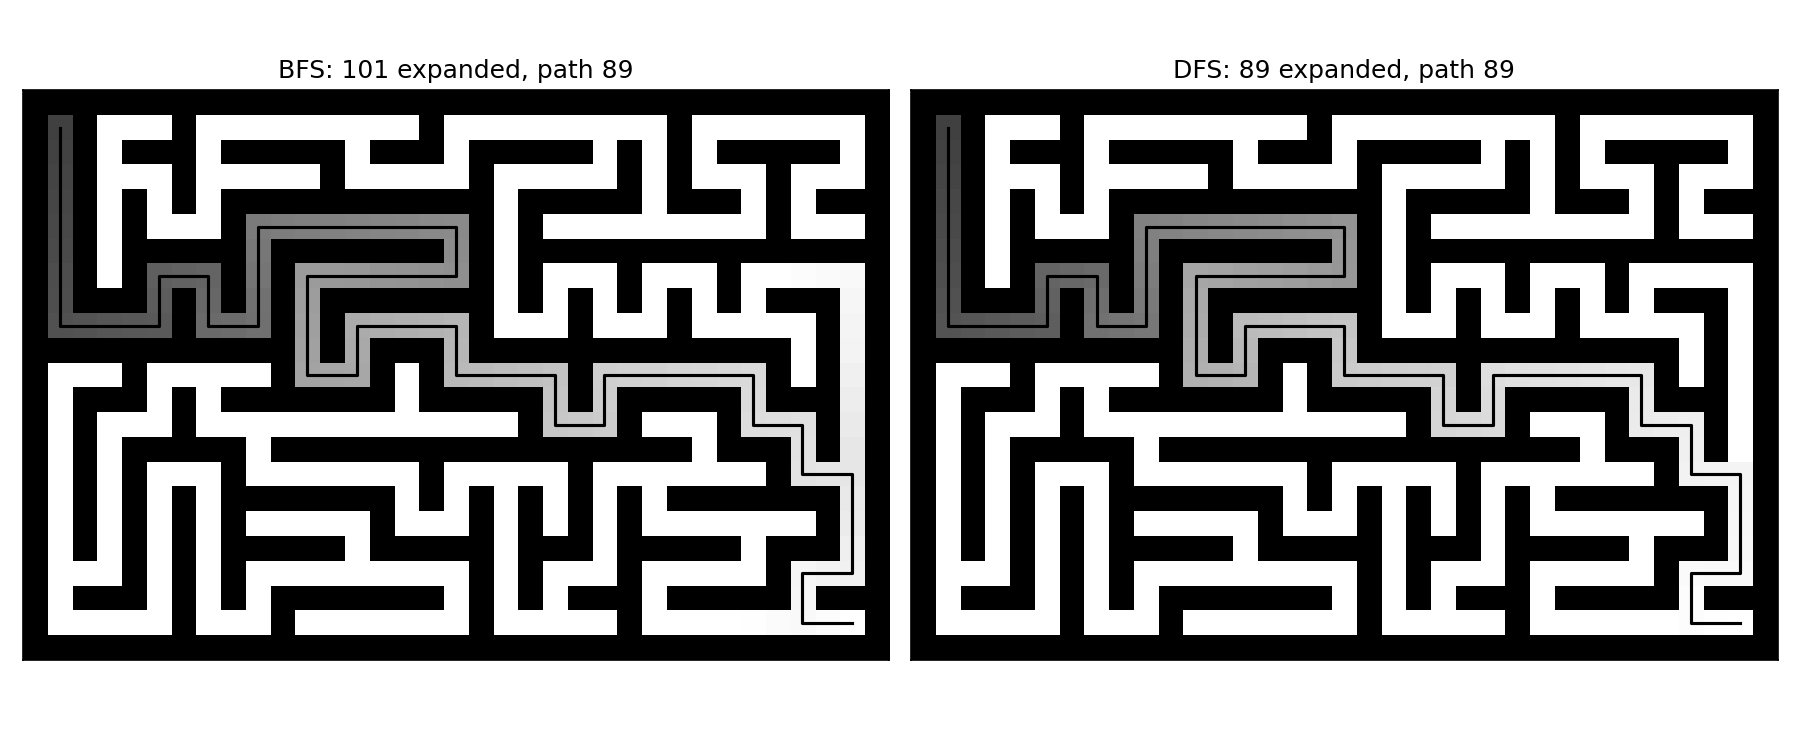
\includegraphics[keepaspectratio,alt={Fig. 3.1 Maze search comparison}]{exp03-search/figs/fig4_1_maze.png}}
\caption{Fig. 3.1 Maze search comparison}
\end{figure}

\subsection{3.9 Observations to record}\label{observations-to-record-2}

Maze dimensions and open cells; cells expanded and path length for both;
validation result.

\subsection{3.10 Applications}\label{applications-2}

Shortest-hop routing, wavefront planner on occupancy grids; topological
sorting, cycle detection, maze carving.

\subsection{3.11 Questions and answers}\label{questions-and-answers-2}

Q1. DFS path 97 and BFS 81: what can you conclude, and what can you not?
A: BFS is optimal (shortest) by guarantee. DFS's path being longer is
expected but not proof that DFS always loses; a different goal placement
could make DFS expand more or fewer cells.

Q2. Why must the bounds check come before the wall check? A: Negative
indices wrap around in NumPy, so checking contents first can read a
valid cell through a wall silently.

Q3. Why mark a cell when enqueued rather than expanded? A: To prevent
the same cell entering the frontier multiple times, keeping complexity
polynomial.

Q4. State space complexity of each; which on a memory-constrained robot?
A: BFS O(b\^{}d) time/space; DFS O(bm) space. Choose DFS when memory is
tight and optimality is not required.

Q5. If diagonal moves were allowed, would BFS still return a shortest
path? Justify. A: Yes, if all moves (including diagonals) have equal
cost; BFS guarantees shortest path in unweighted graphs. If diagonal
cost differs (sqrt2), use Dijkstra/A*.

\begin{figure}
\centering
\pandocbounded{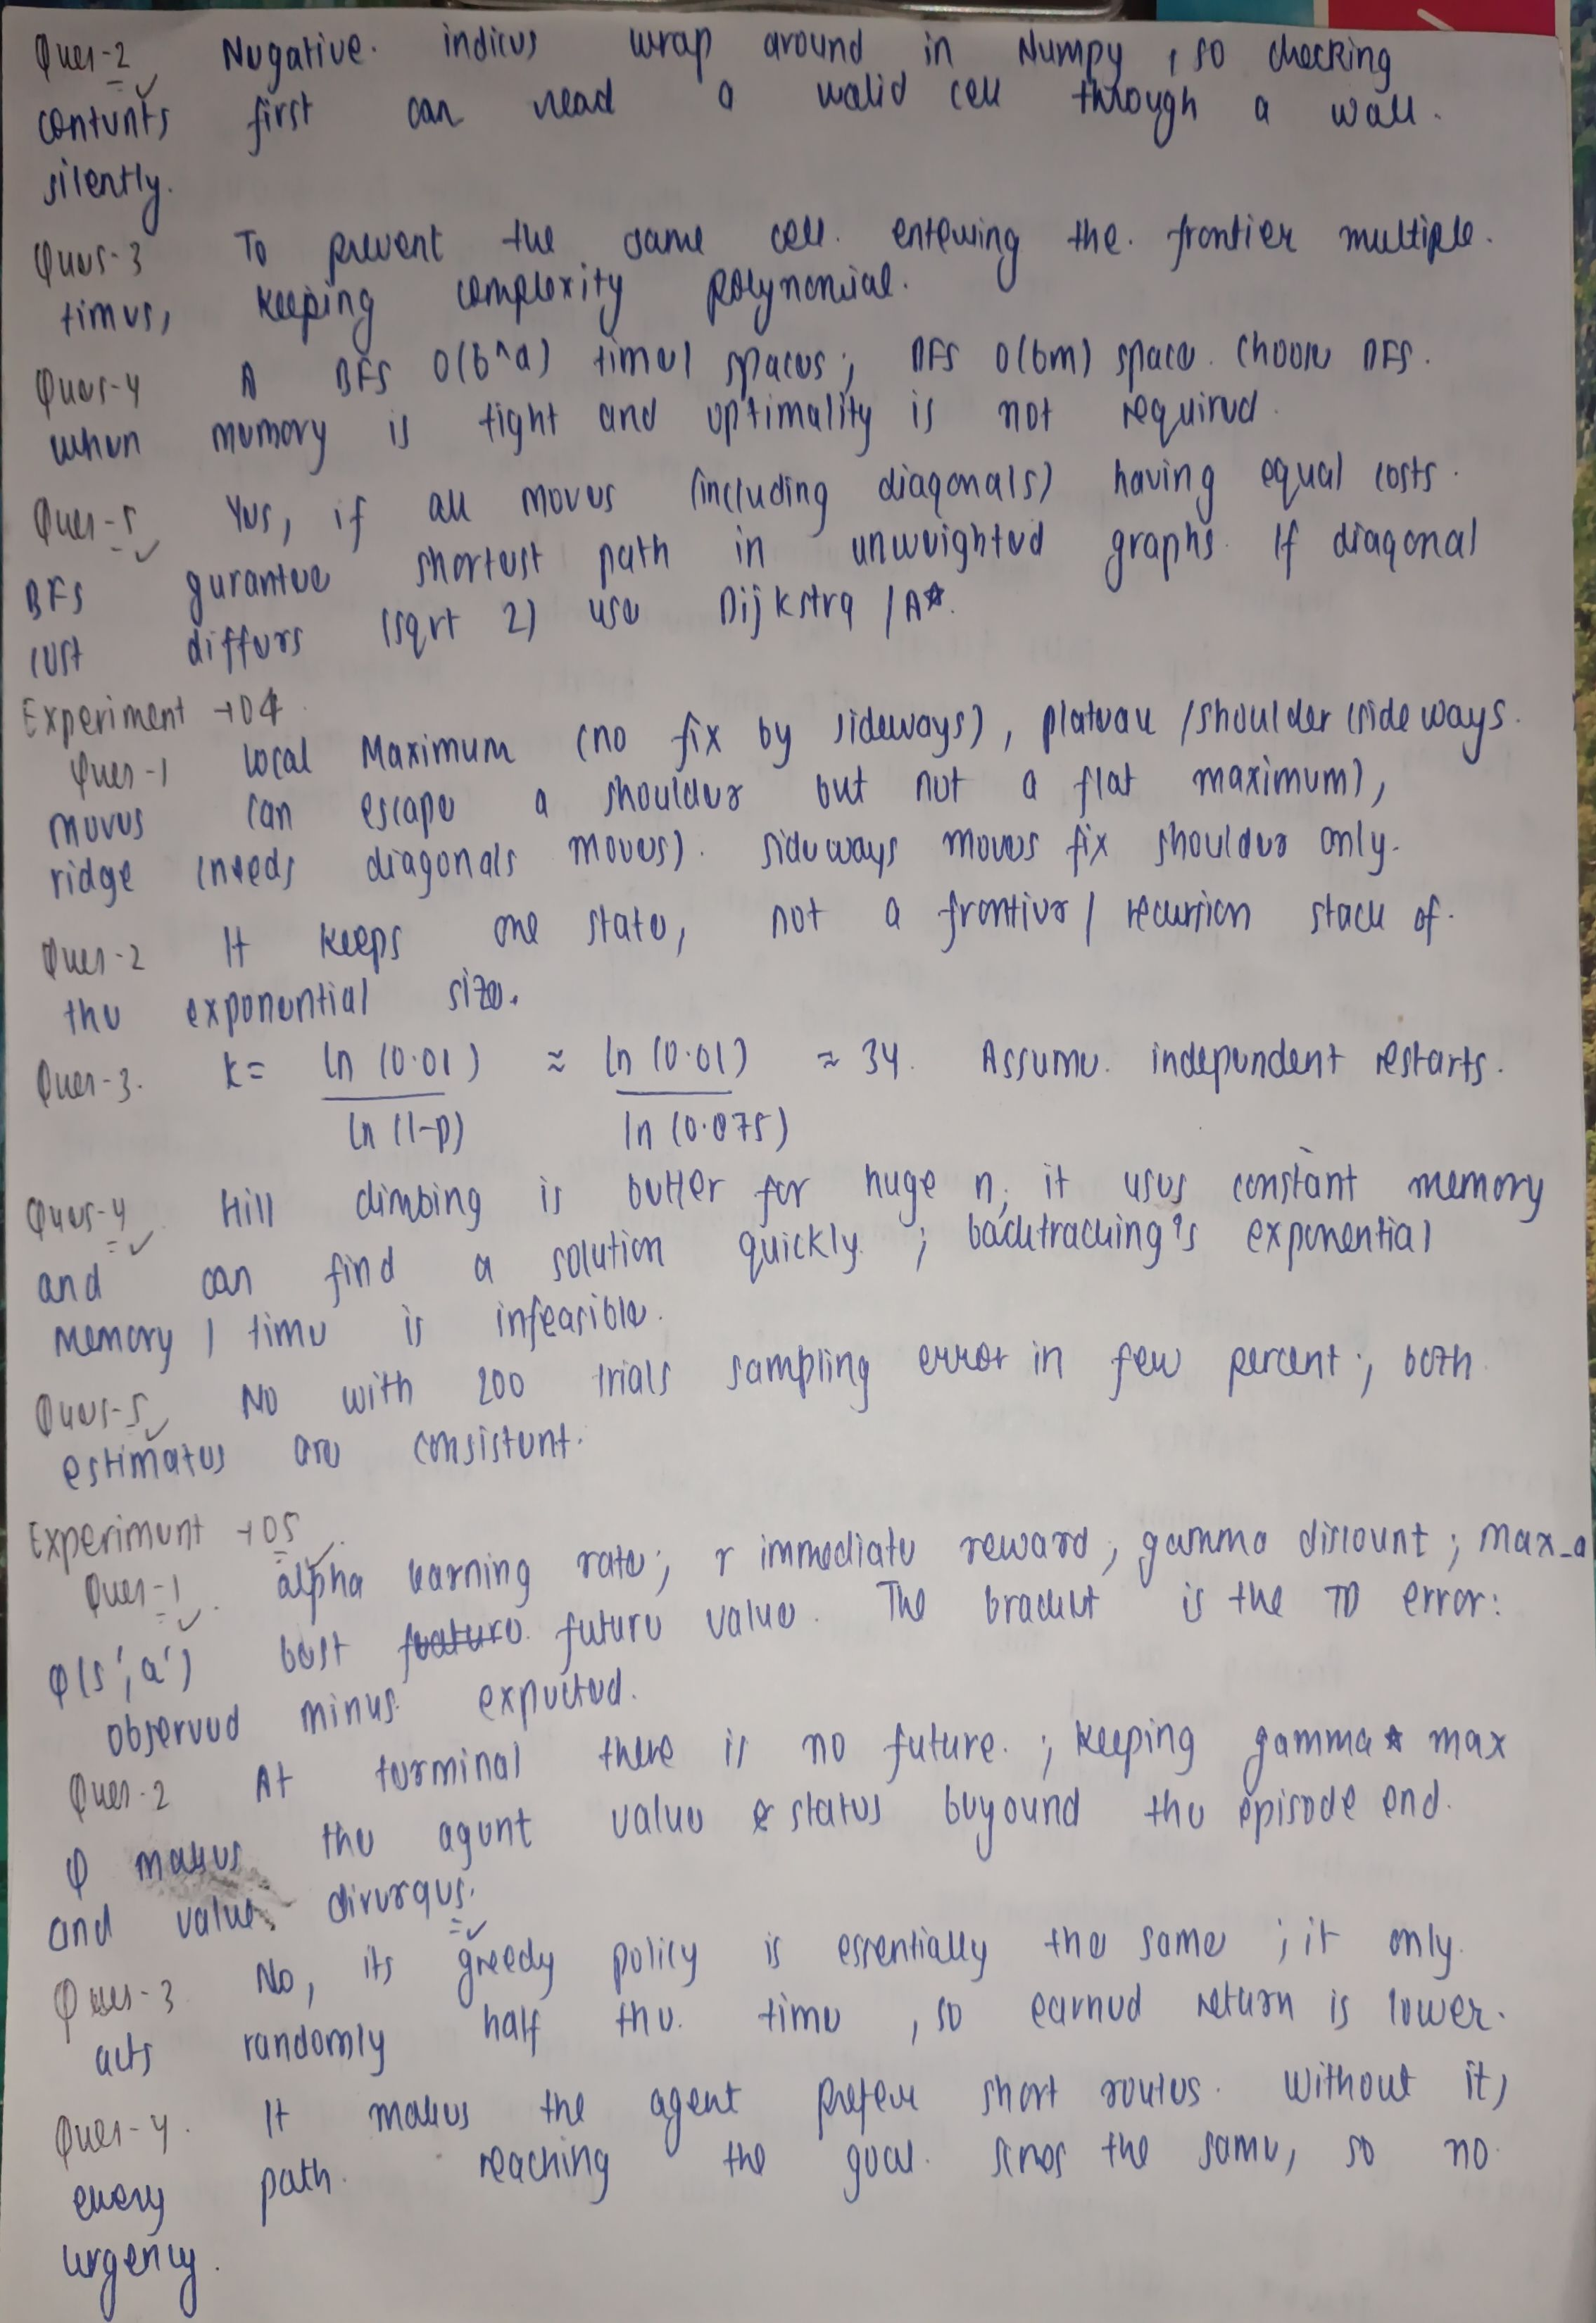
\includegraphics[keepaspectratio,alt={Handwritten answers (scanned) --- page 2}]{handwritten_p2.png}}
\caption{Handwritten answers (scanned) --- page 2}
\end{figure}

\emph{Scanned handwritten answer sheet, page 2, covering this
experiment's Questions section.}

\subsection{3.12 Conclusion}\label{conclusion-2}

BFS guaranteed the shortest path; DFS expanded fewer cells here but gave
no optimality guarantee. The trade-off is between
completeness/optimality (BFS) and memory (DFS).

\begin{center}\rule{0.5\linewidth}{0.5pt}\end{center}

\section{Experiment 4: Hill climbing}\label{experiment-4-hill-climbing}

\subsection{4.1 Aim}\label{aim-3}

To implement hill climbing as local search, observe failure on local
optima, plateaus and ridges, and measure improvement from random
restarts.

\subsection{4.2 Objectives}\label{objectives-3}

\begin{enumerate}
\def\labelenumi{\arabic{enumi}.}
\tightlist
\item
  Distinguish systematic search (frontier) from local search (one
  state).
\item
  Implement steepest-ascent hill climbing on a continuous function and
  on eight queens.
\item
  Identify three ways hill climbing gets stuck.
\item
  Measure success rate and show random restarts' effect.
\end{enumerate}

\subsection{4.3 Place in the syllabus}\label{place-in-the-syllabus-3}

Unit II: local search, potential-field local minima; optimality and
constraints. Unit IV: gradient descent. Contributes to CO1.

\subsection{4.4 Requirements}\label{requirements-3}

Python with NumPy, Matplotlib; conflict counter from Exp 2.

\subsection{4.5 Theory}\label{theory-3}

Local search keeps one state; memory constant, completeness lost.
Steepest-ascent: evaluate all neighbours, move to best, stop when none
better. Fails: local maximum, plateau (shoulder/flat), ridge. Random
restarts: k runs succeed with probability 1-(1-p)\^{}k.

\subsection{4.6 Method}\label{method-3}

\begin{enumerate}
\def\labelenumi{\arabic{enumi}.}
\tightlist
\item
  Plot 1D function with several local maxima.
\item
  Implement hill climbing on eight-queens objective (minimise
  conflicts).
\item
  Run from many random starts; record success rate.
\item
  Wrap in random-restart loop; repeat for several restart counts.
\item
  Plot success rate vs restarts; compare with 1-(1-p)\^{}k.
\end{enumerate}

\subsection{4.7 Procedure and code}\label{procedure-and-code-3}

Run \texttt{exp04-hillclimb/exp04.py}.

\subsection{4.8 Results}\label{results-3}

Table 4.1: Measured over 200 random starts per row, n=8. Plain success p
= 12.5\%.

{\def\LTcaptype{none} % do not increment counter
\begin{longtable}[]{@{}lll@{}}
\toprule\noalign{}
Restarts & Success rate & Predicted 1-(1-p)\^{}k \\
\midrule\noalign{}
\endhead
\bottomrule\noalign{}
\endlastfoot
1 & 14.5\% & 12.5\% \\
2 & 25.5\% & 23.4\% \\
5 & 56.0\% & 48.7\% \\
10 & 78.0\% & 73.7\% \\
20 & 97.5\% & 93.1\% \\
\end{longtable}
}

\begin{figure}
\centering
\pandocbounded{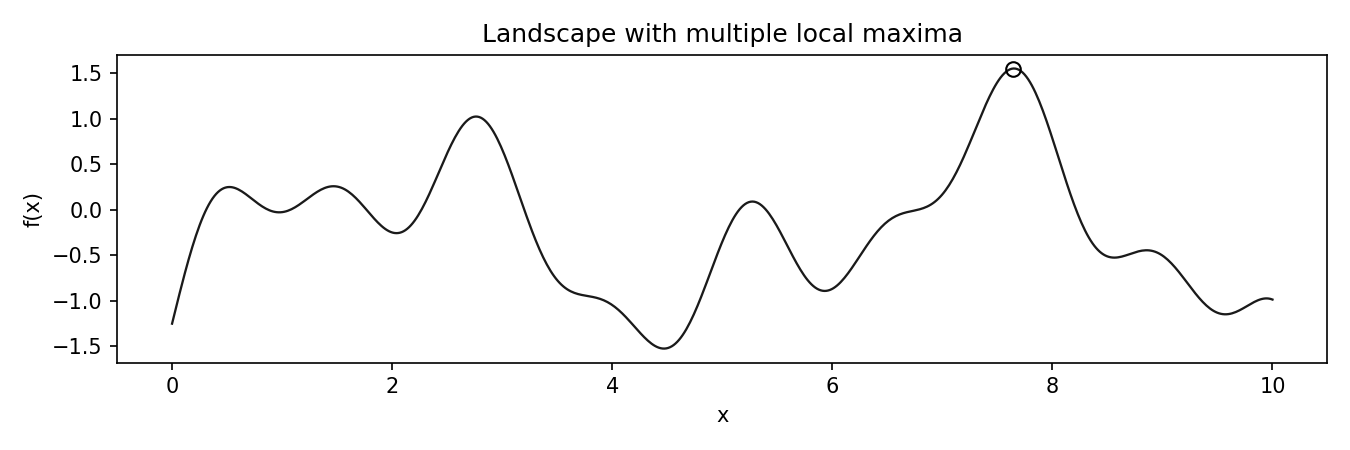
\includegraphics[keepaspectratio,alt={Fig. 4.1 Landscape}]{exp04-hillclimb/figs/fig5_1_landscape.png}}
\caption{Fig. 4.1 Landscape}
\end{figure}

\begin{figure}
\centering
\pandocbounded{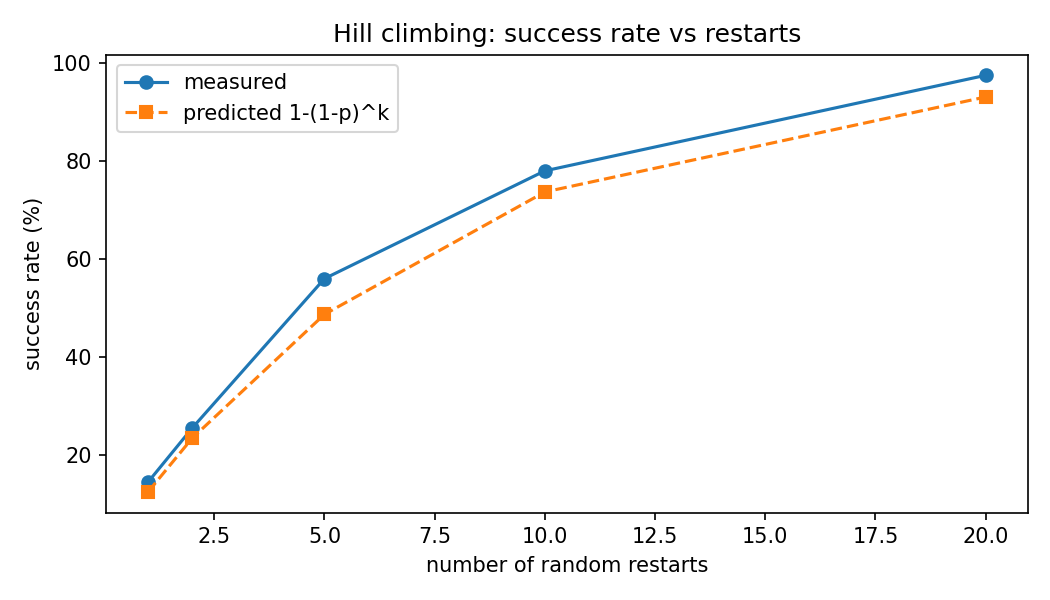
\includegraphics[keepaspectratio,alt={Fig. 4.2 Success rate vs restarts}]{exp04-hillclimb/figs/fig5_2_restarts.png}}
\caption{Fig. 4.2 Success rate vs restarts}
\end{figure}

\subsection{4.9 Observations to record}\label{observations-to-record-3}

Success rate of plain hill climbing over \textgreater=200 starts;
success rate at each restart count; comparison with prediction; number
of trials beside every percentage.

\subsection{4.10 Applications}\label{applications-3}

Large scheduling/layout problems; randomized gradient descent out of
potential-field minima; SGD with multiple initialisations.

\subsection{4.11 Questions and answers}\label{questions-and-answers-3}

Q1. State the three ways hill climbing gets stuck, and say which
sideways moves can fix. A: Local maximum (no fix by sideways),
plateau/shoulder (sideways moves can escape a shoulder but not a flat
maximum), ridge (needs diagonal moves). Sideways moves fix shoulders
only.

Q2. Why does hill climbing use constant memory when backtracking does
not? A: It keeps one state, not a frontier/recursion stack of
exponential size.

Q3. Success rate 15.5\% (12.5\% here). How many restarts for 99\%
success, and what assumption? A: k = ln(0.01)/ln(1-p) \textasciitilde{}
ln(0.01)/ln(0.875) \textasciitilde{} 34. Assumes independent restarts.

Q4. Hill climbing starts with a complete board; backtracking builds
column by column. Which is better for n=1000, and why? A: Hill climbing
is better for huge n: it uses constant memory and can find a solution
quickly; backtracking's exponential memory/time is infeasible.

Q5. 12.5\% on one run and 15.5\% on another. Is the program wrong?
Justify. A: No: with 200 trials sampling error is a few percent; both
estimates are consistent.

\begin{figure}
\centering
\pandocbounded{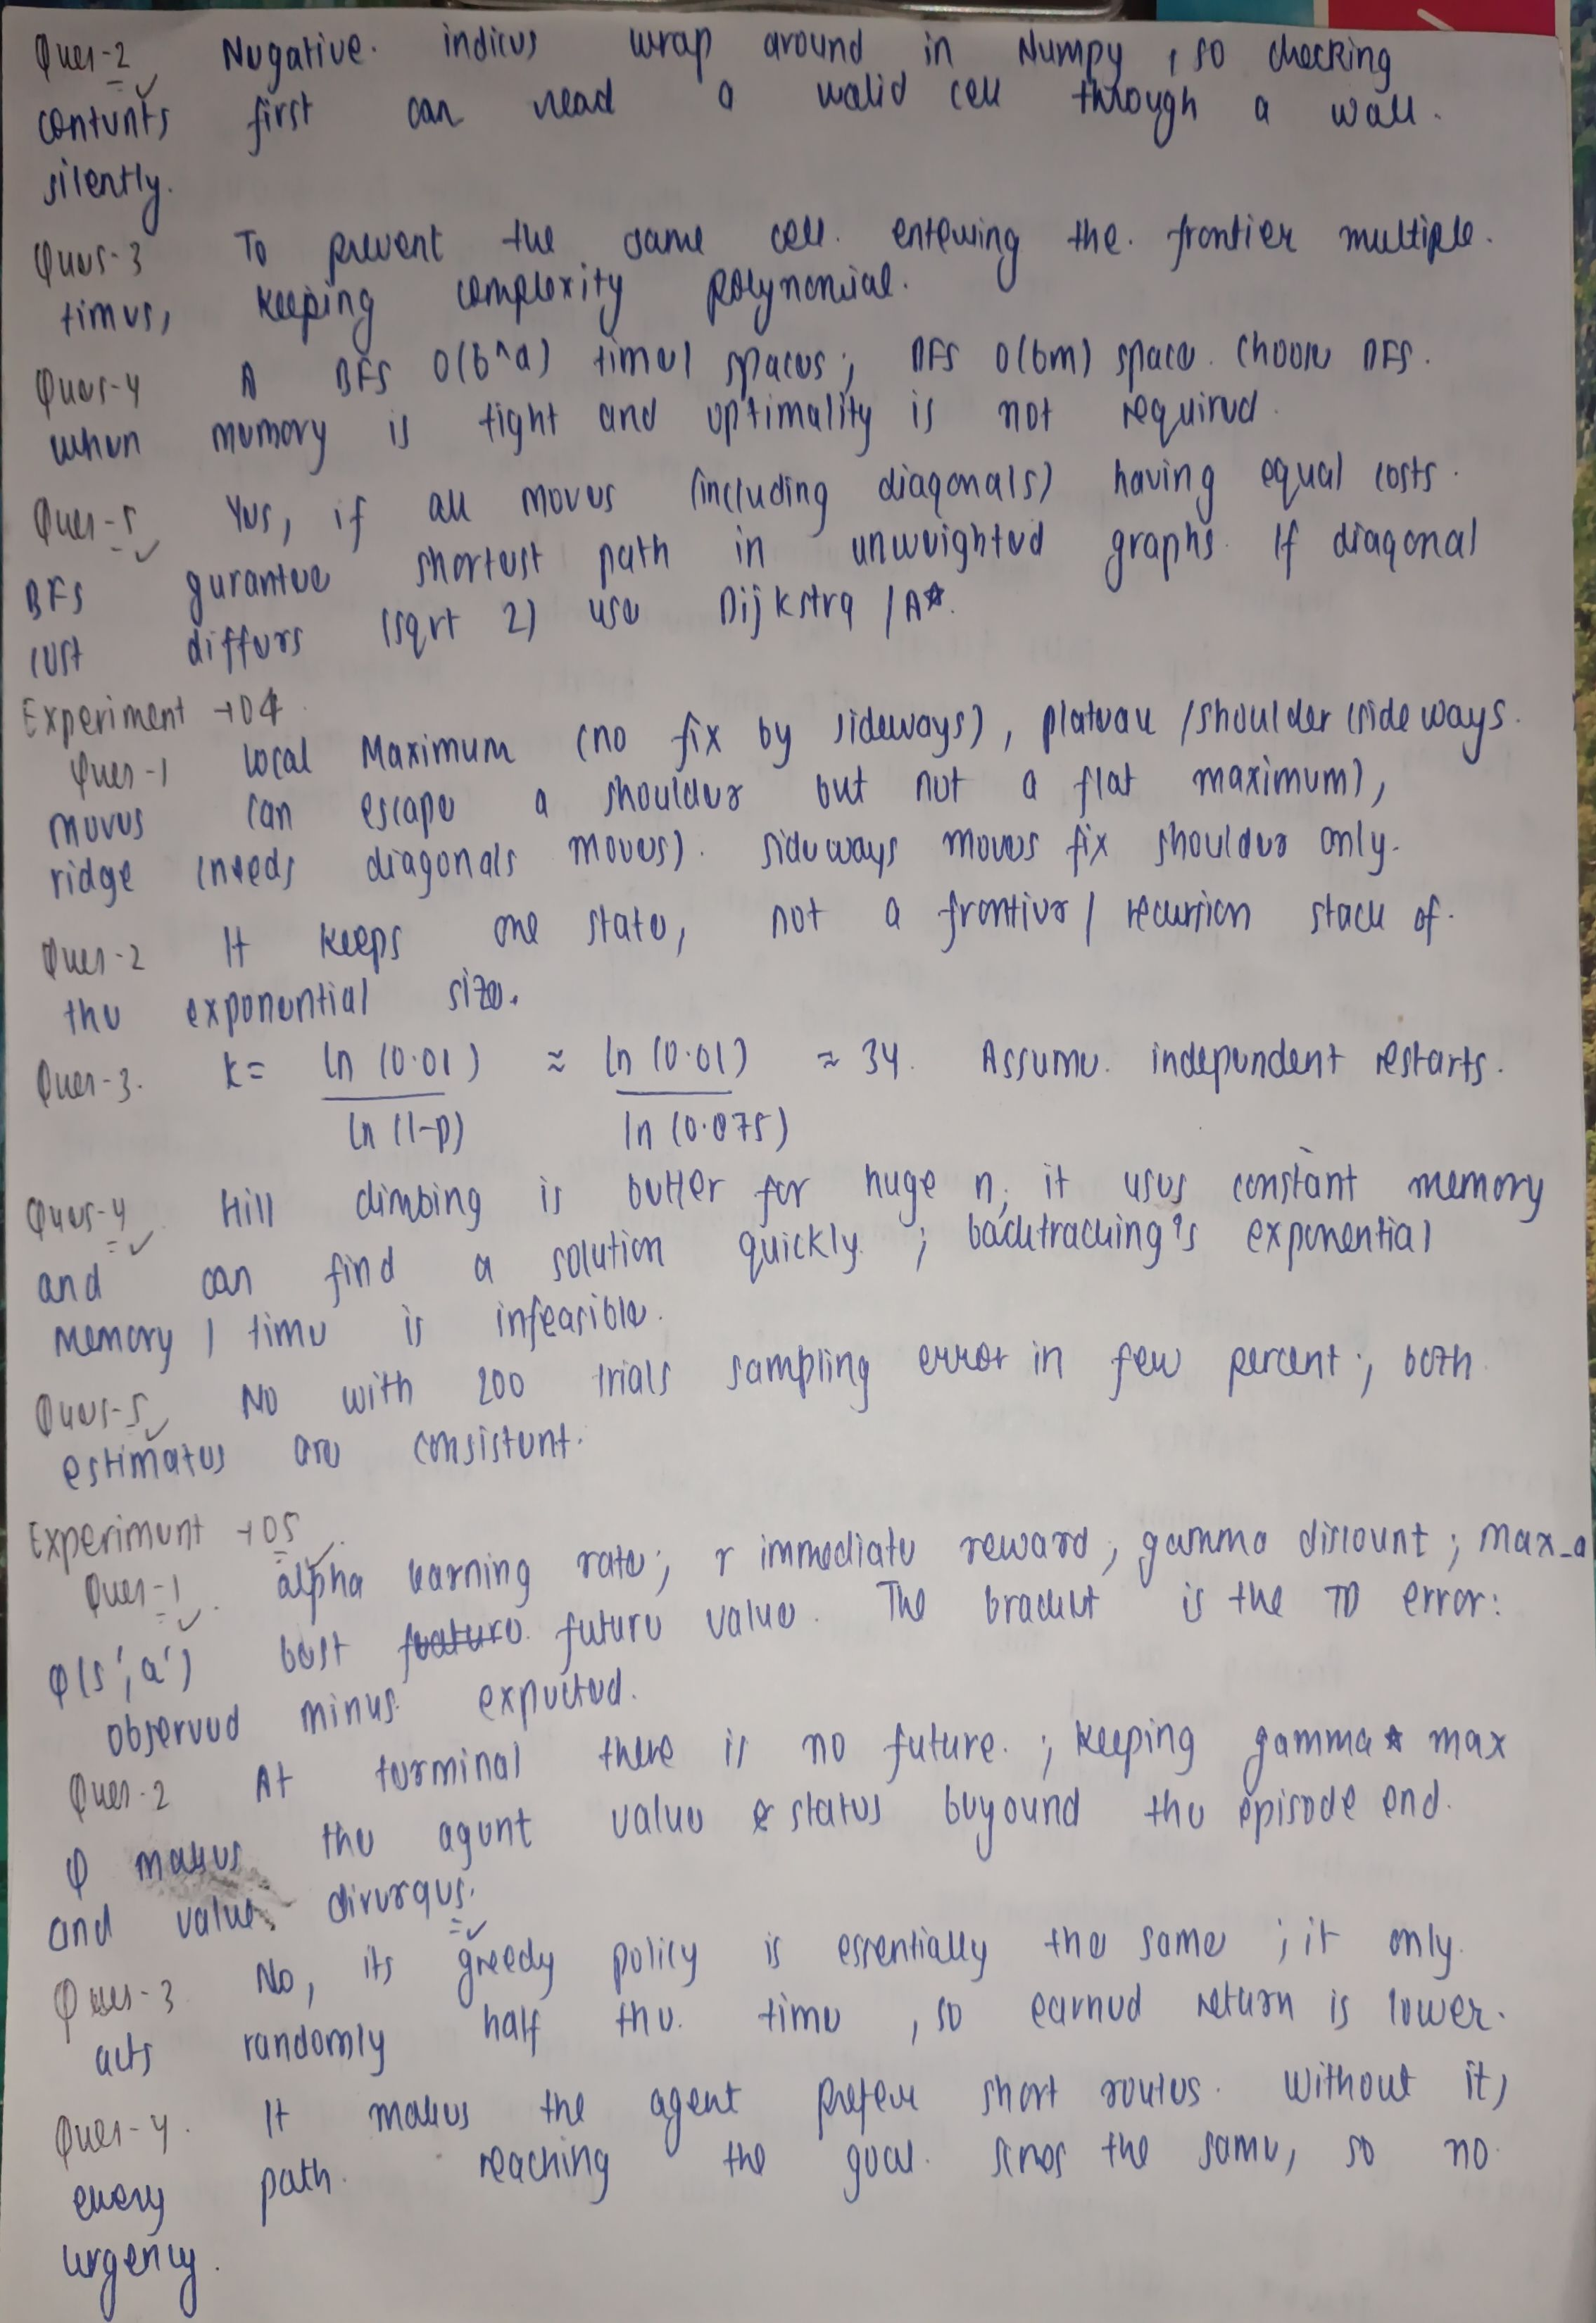
\includegraphics[keepaspectratio,alt={Handwritten answers (scanned) --- page 2}]{handwritten_p2.png}}
\caption{Handwritten answers (scanned) --- page 2}
\end{figure}

\emph{Scanned handwritten answer sheet, page 2, covering this
experiment's Questions section.}

\subsection{4.12 Conclusion}\label{conclusion-3}

Plain hill climbing succeeded \textasciitilde12.5\% of the time; random
restarts raised success to 97.5\% at 20 restarts, tracking the
independence prediction.

\section{Experiment 5: Reinforcement
learning}\label{experiment-5-reinforcement-learning}

\subsection{5.1 Aim}\label{aim-4}

To formulate a navigation task as a Markov decision process, implement
Q-learning on a grid world, and measure the effect of exploration rate
on what is learned and how quickly.

\subsection{5.2 Objectives}\label{objectives-4}

\begin{enumerate}
\def\labelenumi{\arabic{enumi}.}
\tightlist
\item
  State a task as states, actions, transitions, rewards.
\item
  Implement tabular Q-learning and explain each term.
\item
  Show why exploration is necessary and its cost.
\item
  Extract and display a policy from the Q table.
\end{enumerate}

\subsection{5.3 Place in the syllabus}\label{place-in-the-syllabus-4}

Unit I: learning agent. Unit IV: ML concepts, RL as third branch. Unit
II: learned policy as feedback controller. Contributes to CO1.

\subsection{5.4 Requirements}\label{requirements-4}

Python with NumPy, Matplotlib.

\subsection{5.5 Theory}\label{theory-4}

MDP: states s, actions a, transitions, rewards r. Q-learning update:
Q(s,a) \textless- Q(s,a) + alpha {[} r + gamma max\_a' Q(s',a') - Q(s,a)
{]}. TD error in brackets. Off-policy via max. Epsilon-greedy
exploration. Step cost -0.1 makes agent prefer short routes.

\subsection{5.6 Method}\label{method-4}

\begin{enumerate}
\def\labelenumi{\arabic{enumi}.}
\tightlist
\item
  Define grid world with walls, goal +10, pit -10, step cost -0.1.
\item
  Initialise Q to zero.
\item
  For each episode, act epsilon-greedy, update after every step, stop at
  terminal or step cap (120).
\item
  Record total reward per episode.
\item
  Repeat for several epsilon; plot smoothed learning curves.
\item
  Extract greedy policy; draw arrows.
\end{enumerate}

\subsection{5.7 Procedure and code}\label{procedure-and-code-4}

Run \texttt{exp05-rl/exp05.py}.

\subsection{5.8 Results}\label{results-4}

Table 5.1: Mean return over final 100 episodes of a 600-episode run.

{\def\LTcaptype{none} % do not increment counter
\begin{longtable}[]{@{}lll@{}}
\toprule\noalign{}
epsilon & Mean return, last 100 & Interpretation \\
\midrule\noalign{}
\endhead
\bottomrule\noalign{}
\endlastfoot
0.05 & 8.86 & Learns well; slowest to discover goal at first \\
0.20 & 8.86 & Same final quality, faster early progress \\
0.50 & 7.44 & Same policy learned, but acts randomly half the time \\
\end{longtable}
}

Extracted policy (epsilon=0.20) routes around the pit to the goal.

\begin{figure}
\centering
\pandocbounded{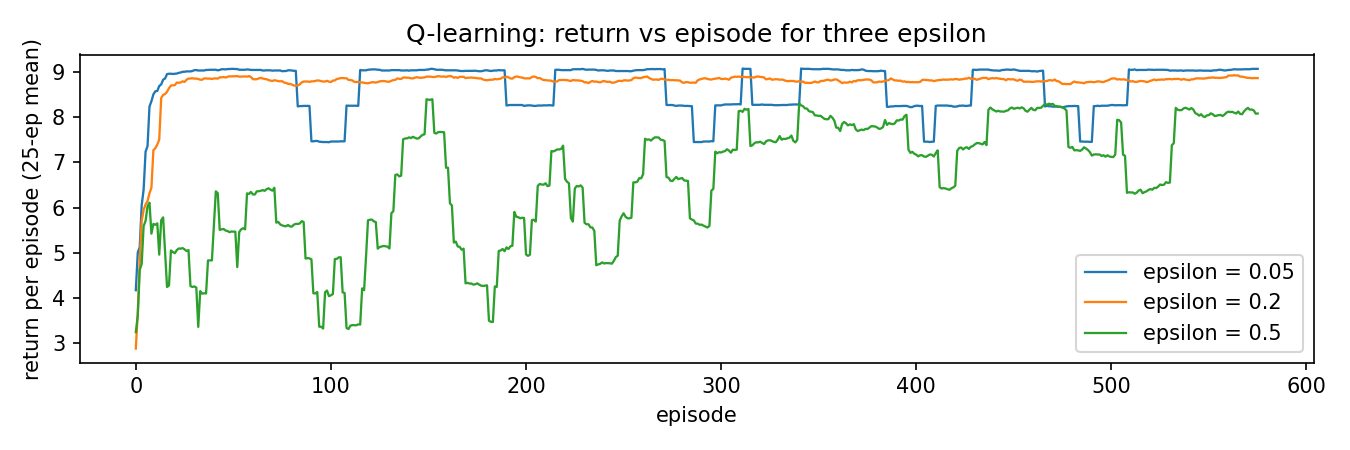
\includegraphics[keepaspectratio,alt={Fig. 5.1 Q-learning return vs episode}]{exp05-rl/figs/fig6_1_learning.png}}
\caption{Fig. 5.1 Q-learning return vs episode}
\end{figure}

\subsection{5.9 Observations to record}\label{observations-to-record-4}

Grid dimensions, reward structure, alpha, gamma, episodes, mean return
over last 100 for each epsilon, extracted policy grid.

\subsection{5.10 Applications}\label{applications-4}

Robot locomotion gaits, manipulation policies in simulation, data-centre
cooling, traffic signals. Tabular Q-learning does not scale; DQN
replaces the table.

\subsection{5.11 Questions and answers}\label{questions-and-answers-4}

Q1. Explain each term of the Q-learning update, and say what the bracket
represents. A: alpha learning rate; r immediate reward; gamma discount;
max\_a' Q(s',a') best future value. The bracket is the TD error:
observed minus expected.

Q2. Why must the future-value term be dropped at a terminal state? A: At
terminal there is no future; keeping gamma*max Q makes the agent value
states beyond the episode end and values diverge.

Q3. The epsilon=0.5 agent earns less. Has it learned a worse policy?
Justify. A: No: its greedy policy is essentially the same; it only acts
randomly half the time, so earned return is lower.

Q4. Purpose of -0.1 reward per step? What happens without it? A: It
makes the agent prefer short routes. Without it, every path reaching the
goal scores the same, so no urgency.

Q5. Q-learning is off-policy. What does that mean, and why does it
permit exploration? A: It learns the value of the best (greedy) action
while behaving epsilon-greedily; the max decouples learning from
behaviour, so exploration does not corrupt the target.

\begin{figure}
\centering
\pandocbounded{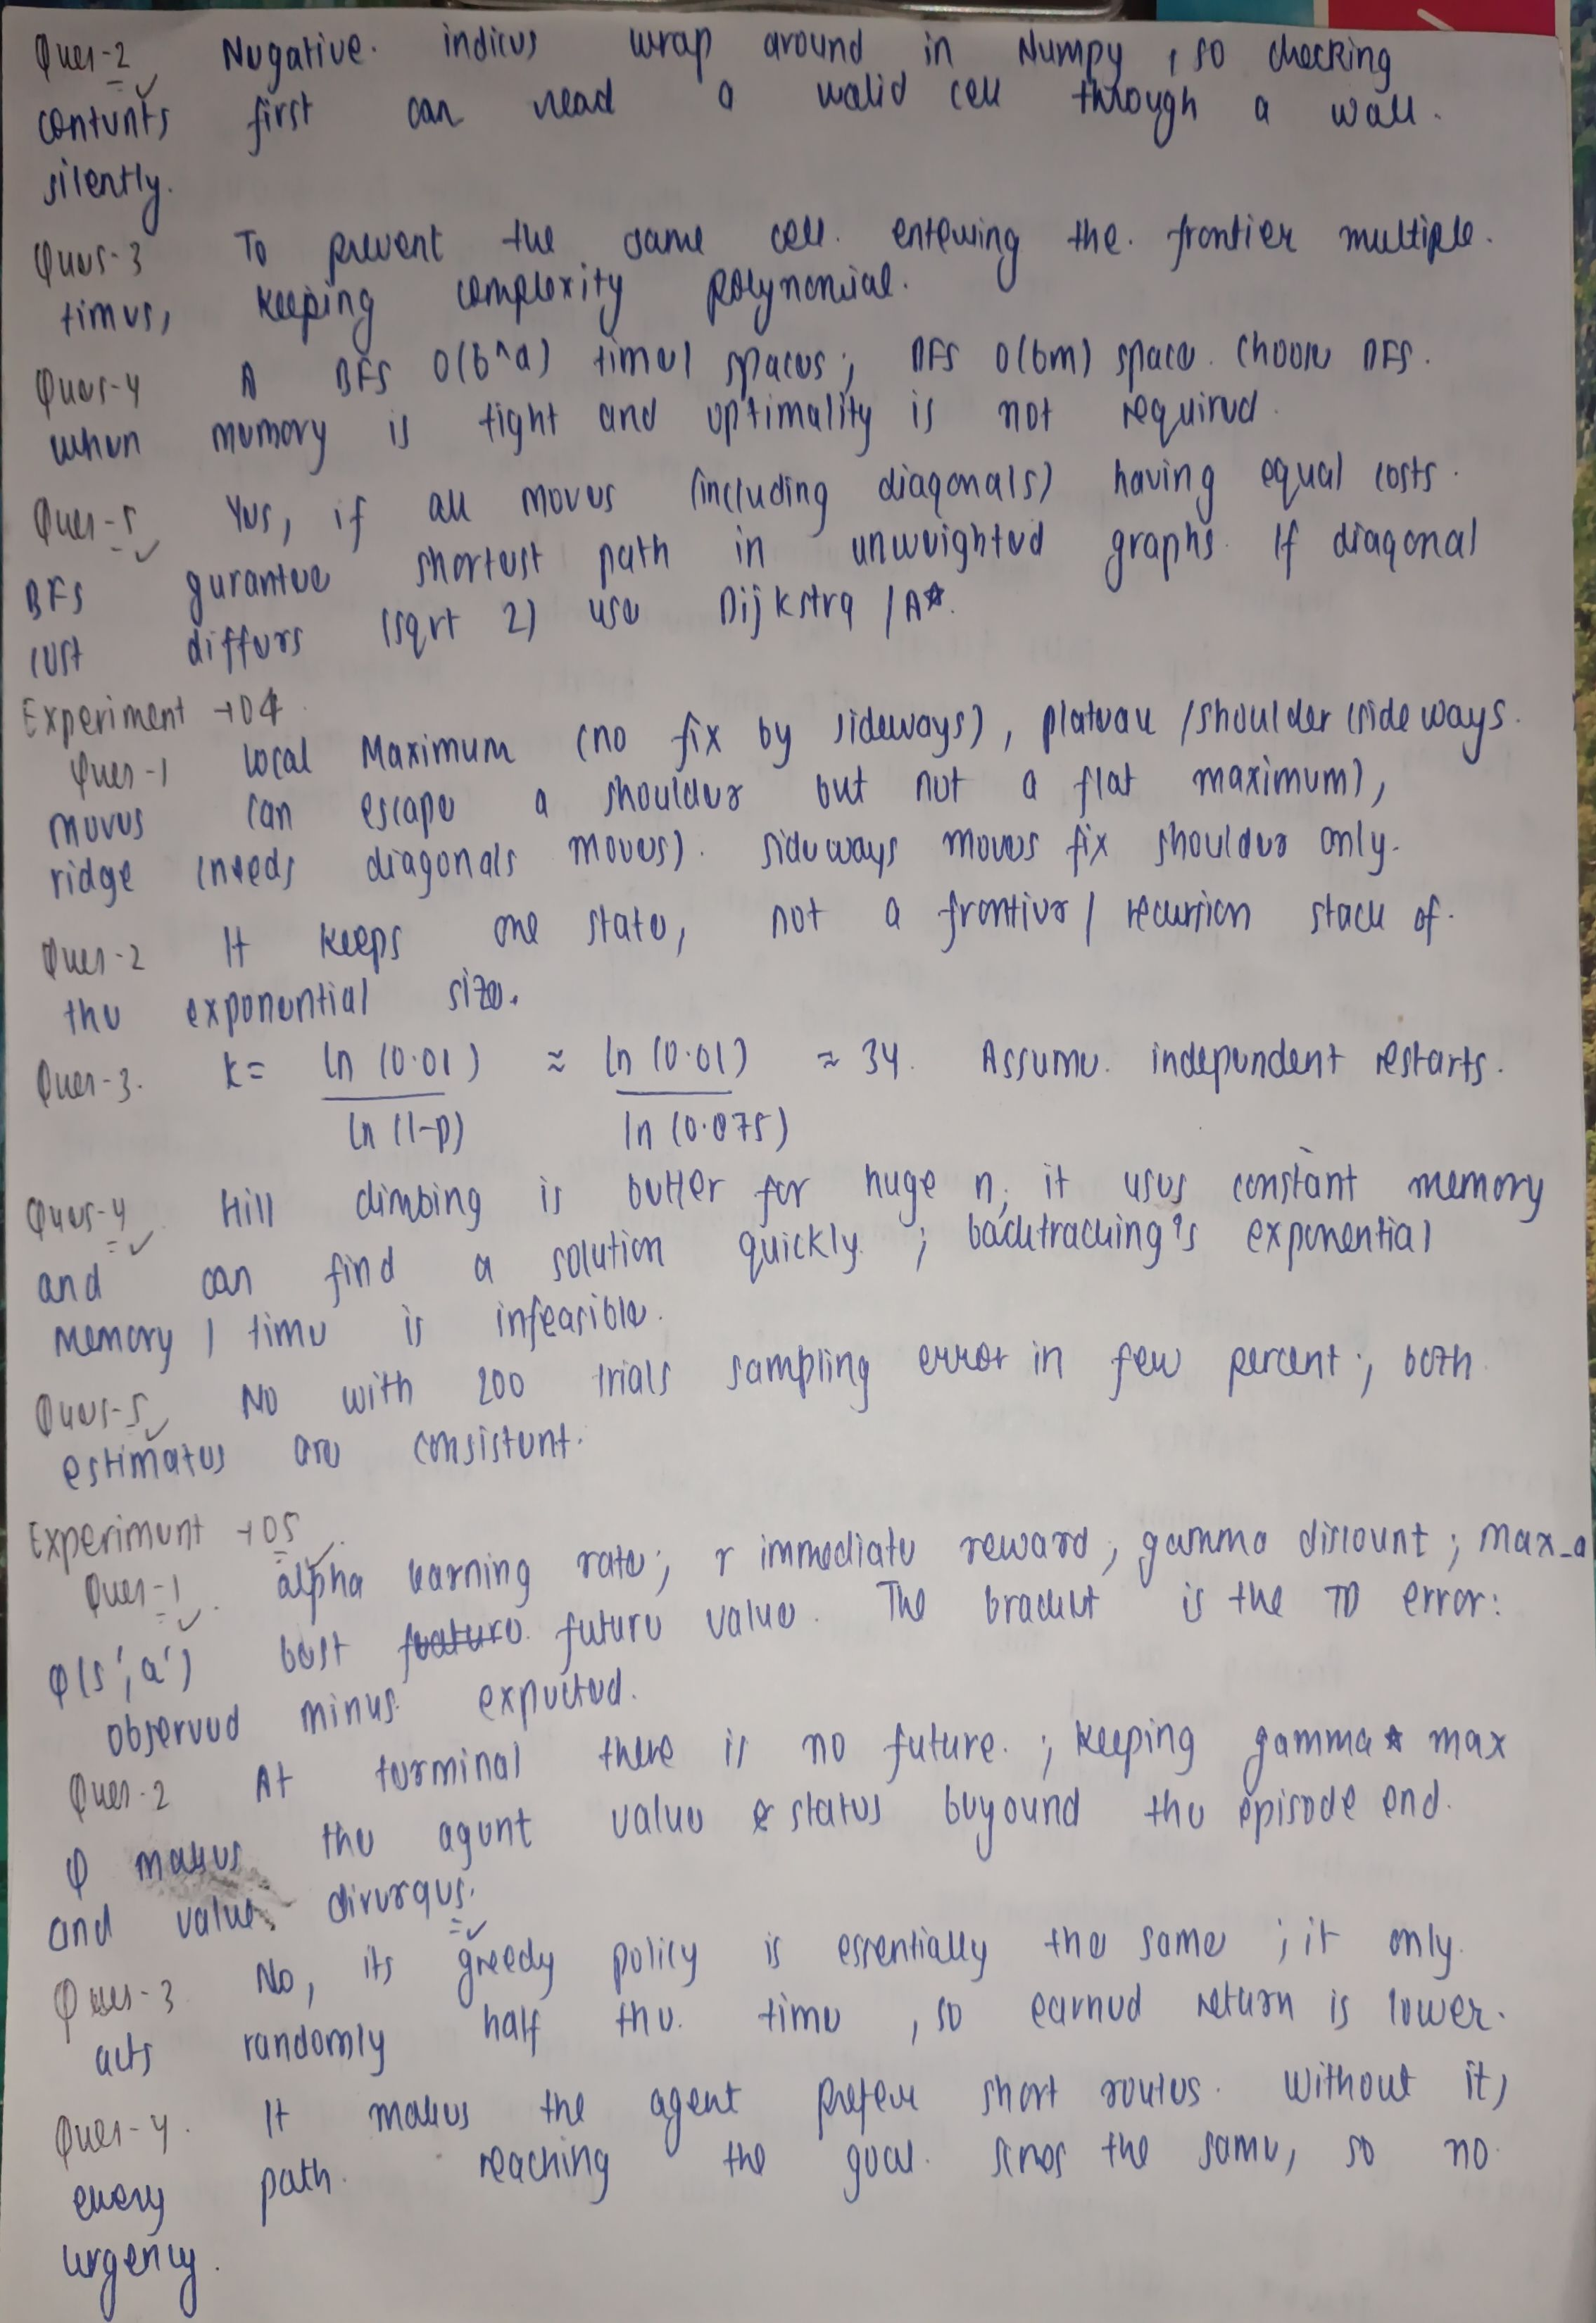
\includegraphics[keepaspectratio,alt={Handwritten answers (scanned) --- page 2}]{handwritten_p2.png}}
\caption{Handwritten answers (scanned) --- page 2}
\end{figure}

\emph{Scanned handwritten answer sheet, page 2, covering this
experiment's Questions section.}

\subsection{5.12 Conclusion}\label{conclusion-4}

All three epsilon values learned a good policy; higher epsilon lowered
earned return without worsening the learned policy, illustrating the
distinction between learned policy and exhibited behaviour.

\begin{center}\rule{0.5\linewidth}{0.5pt}\end{center}

\section{Experiment 6: A simple neural
network}\label{experiment-6-a-simple-neural-network}

\subsection{6.1 Aim}\label{aim-5}

To implement a two-layer neural network in NumPy alone, train it on XOR
by backpropagation, and observe the effect of learning rate on
convergence.

\subsection{6.2 Objectives}\label{objectives-5}

\begin{enumerate}
\def\labelenumi{\arabic{enumi}.}
\tightlist
\item
  Show why a single linear unit cannot represent XOR.
\item
  Implement forward pass, loss, backpropagation, gradient descent
  without a framework.
\item
  Train to convergence and verify the learned function.
\item
  Measure learning-rate effect and visualise the decision boundary.
\end{enumerate}

\subsection{6.3 Place in the syllabus}\label{place-in-the-syllabus-5}

Unit IV: ML concepts, supervised branch. Unit IV: gradient descent as
hill climbing on a differentiable landscape. Unit V: inductive vs
knowledge-based learning. Contributes to CO1.

\subsection{6.4 Requirements}\label{requirements-5}

Python with NumPy, Matplotlib. No ML framework.

\subsection{6.5 Theory}\label{theory-5}

Single linear unit cannot separate XOR (not linearly separable). Hidden
layer re-represents input. Network: h = sigmoid(W1 x + b1), o =
sigmoid(W2 h + b2). Loss E = mean (o-y)\^{}2. Deltas: do = (o-y) o(1-o);
dh = (do W2\^{}T) h(1-h). Weights must be initialised randomly (zero
init makes hidden units identical).

\subsection{6.6 Method}\label{method-5}

\begin{enumerate}
\def\labelenumi{\arabic{enumi}.}
\tightlist
\item
  Write four XOR pairs.
\item
  Initialise weights randomly (seeded), biases zero.
\item
  Implement forward pass and loss.
\item
  Derive and implement deltas and gradients.
\item
  Update by gradient descent; record loss per epoch.
\item
  Repeat for several learning rates; plot on log axis.
\item
  Evaluate on dense grid; plot decision boundary.
\end{enumerate}

\subsection{6.7 Procedure and code}\label{procedure-and-code-5}

Run \texttt{exp06-neural/exp06.py}.

\subsection{6.8 Results}\label{results-5}

Table 6.1: Final MSE after 20000 epochs, 4 hidden units, seed 1.

{\def\LTcaptype{none} % do not increment counter
\begin{longtable}[]{@{}lll@{}}
\toprule\noalign{}
Learning rate & Final MSE & Behaviour \\
\midrule\noalign{}
\endhead
\bottomrule\noalign{}
\endlastfoot
0.05 & 2.31e-03 & Still descending; not converged \\
0.50 & 1.11e-04 & Converged \\
2.00 & 2.46e-05 & Converged fastest, no instability \\
10.00 & 5.81e-06 & Converged (tiny problem only) \\
\end{longtable}
}

Predictions at lr=2.0: {[}0.004, 0.995, 0.996, 0.006{]} (XOR). lr=10.0
would diverge on larger networks.

\begin{figure}
\centering
\pandocbounded{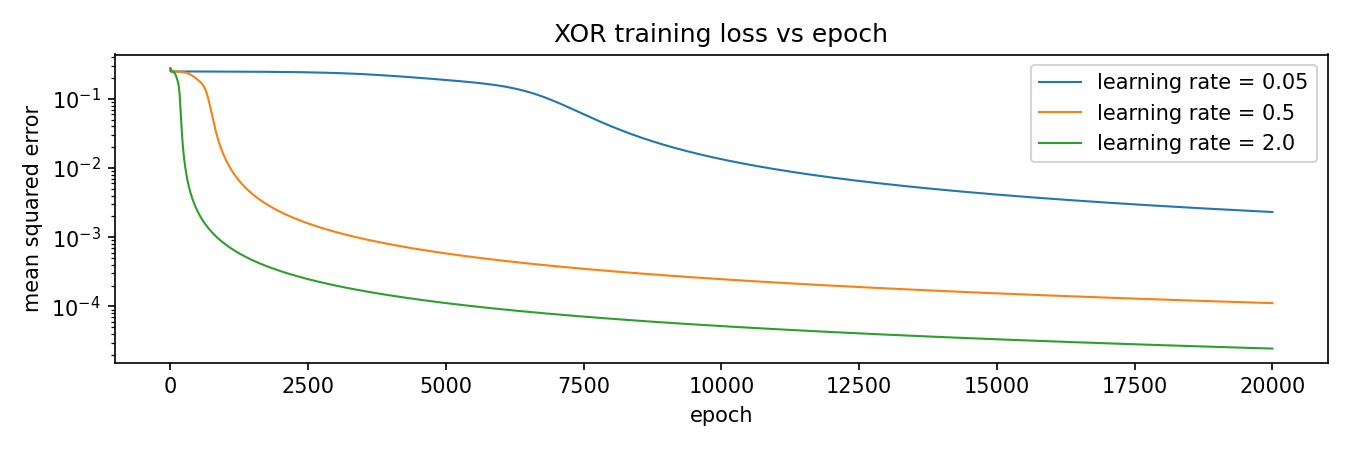
\includegraphics[keepaspectratio,alt={Fig. 6.1 XOR training loss}]{exp06-neural/figs/fig7_1_loss.png}}
\caption{Fig. 6.1 XOR training loss}
\end{figure}

\begin{figure}
\centering
\pandocbounded{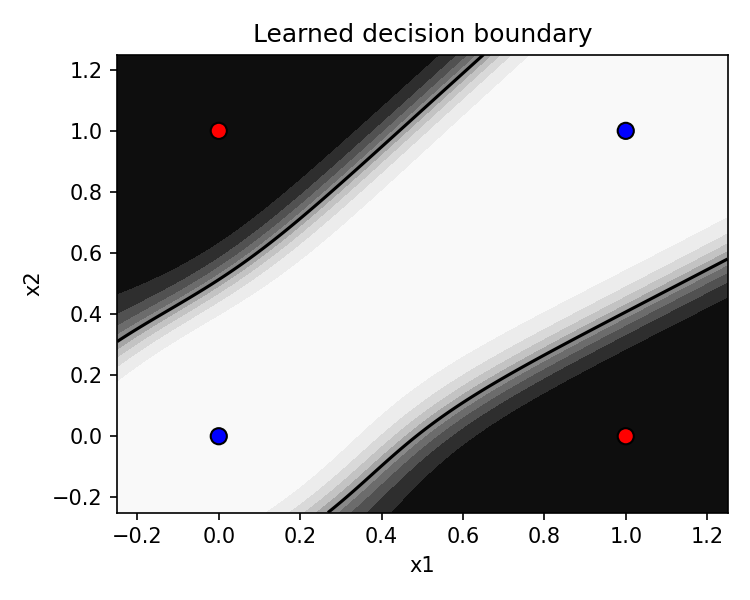
\includegraphics[keepaspectratio,alt={Fig. 6.2 Decision boundary}]{exp06-neural/figs/fig7_2_boundary.png}}
\caption{Fig. 6.2 Decision boundary}
\end{figure}

\subsection{6.9 Observations to record}\label{observations-to-record-5}

Network shape, init seed, learning rates tried, loss curve per rate,
final MSE, four predicted outputs rounded to 3 decimals, convergence
statement.

\subsection{6.10 Applications}\label{applications-5}

Object recognition on a robot camera, learned inverse kinematics, value
approximators replacing Q-tables.

\subsection{6.11 Questions and answers}\label{questions-and-answers-5}

Q1. Why can a single linear unit not represent XOR? What does the hidden
layer change? A: XOR is not linearly separable; no single line splits
(0,0),(1,1) from (0,1),(1,0). The hidden layer re-represents input in a
space where it becomes separable.

Q2. What goes wrong if all weights are initialised to zero, and why? A:
All hidden units compute identically and receive identical gradients,
staying identical forever; the network reduces to a single unit and
cannot learn XOR.

Q3. Where does o(1-o) come from in the output delta? A: It is the
derivative of the sigmoid: sigma'(z) = sigma(z)(1-sigma(z)), expressed
via the activation o.

Q4. Loss flat for thousands of epochs then falls sharply. What is
happening? A: The network sits near the symmetric initial solution
before hidden units differentiate; once symmetry breaks, learning
accelerates.

Q5. Which earlier experiment is gradient descent a continuous version
of, and what failure mode do they share? A: Hill climbing (Exp 4); both
can get stuck in local minima.

\begin{figure}
\centering
\pandocbounded{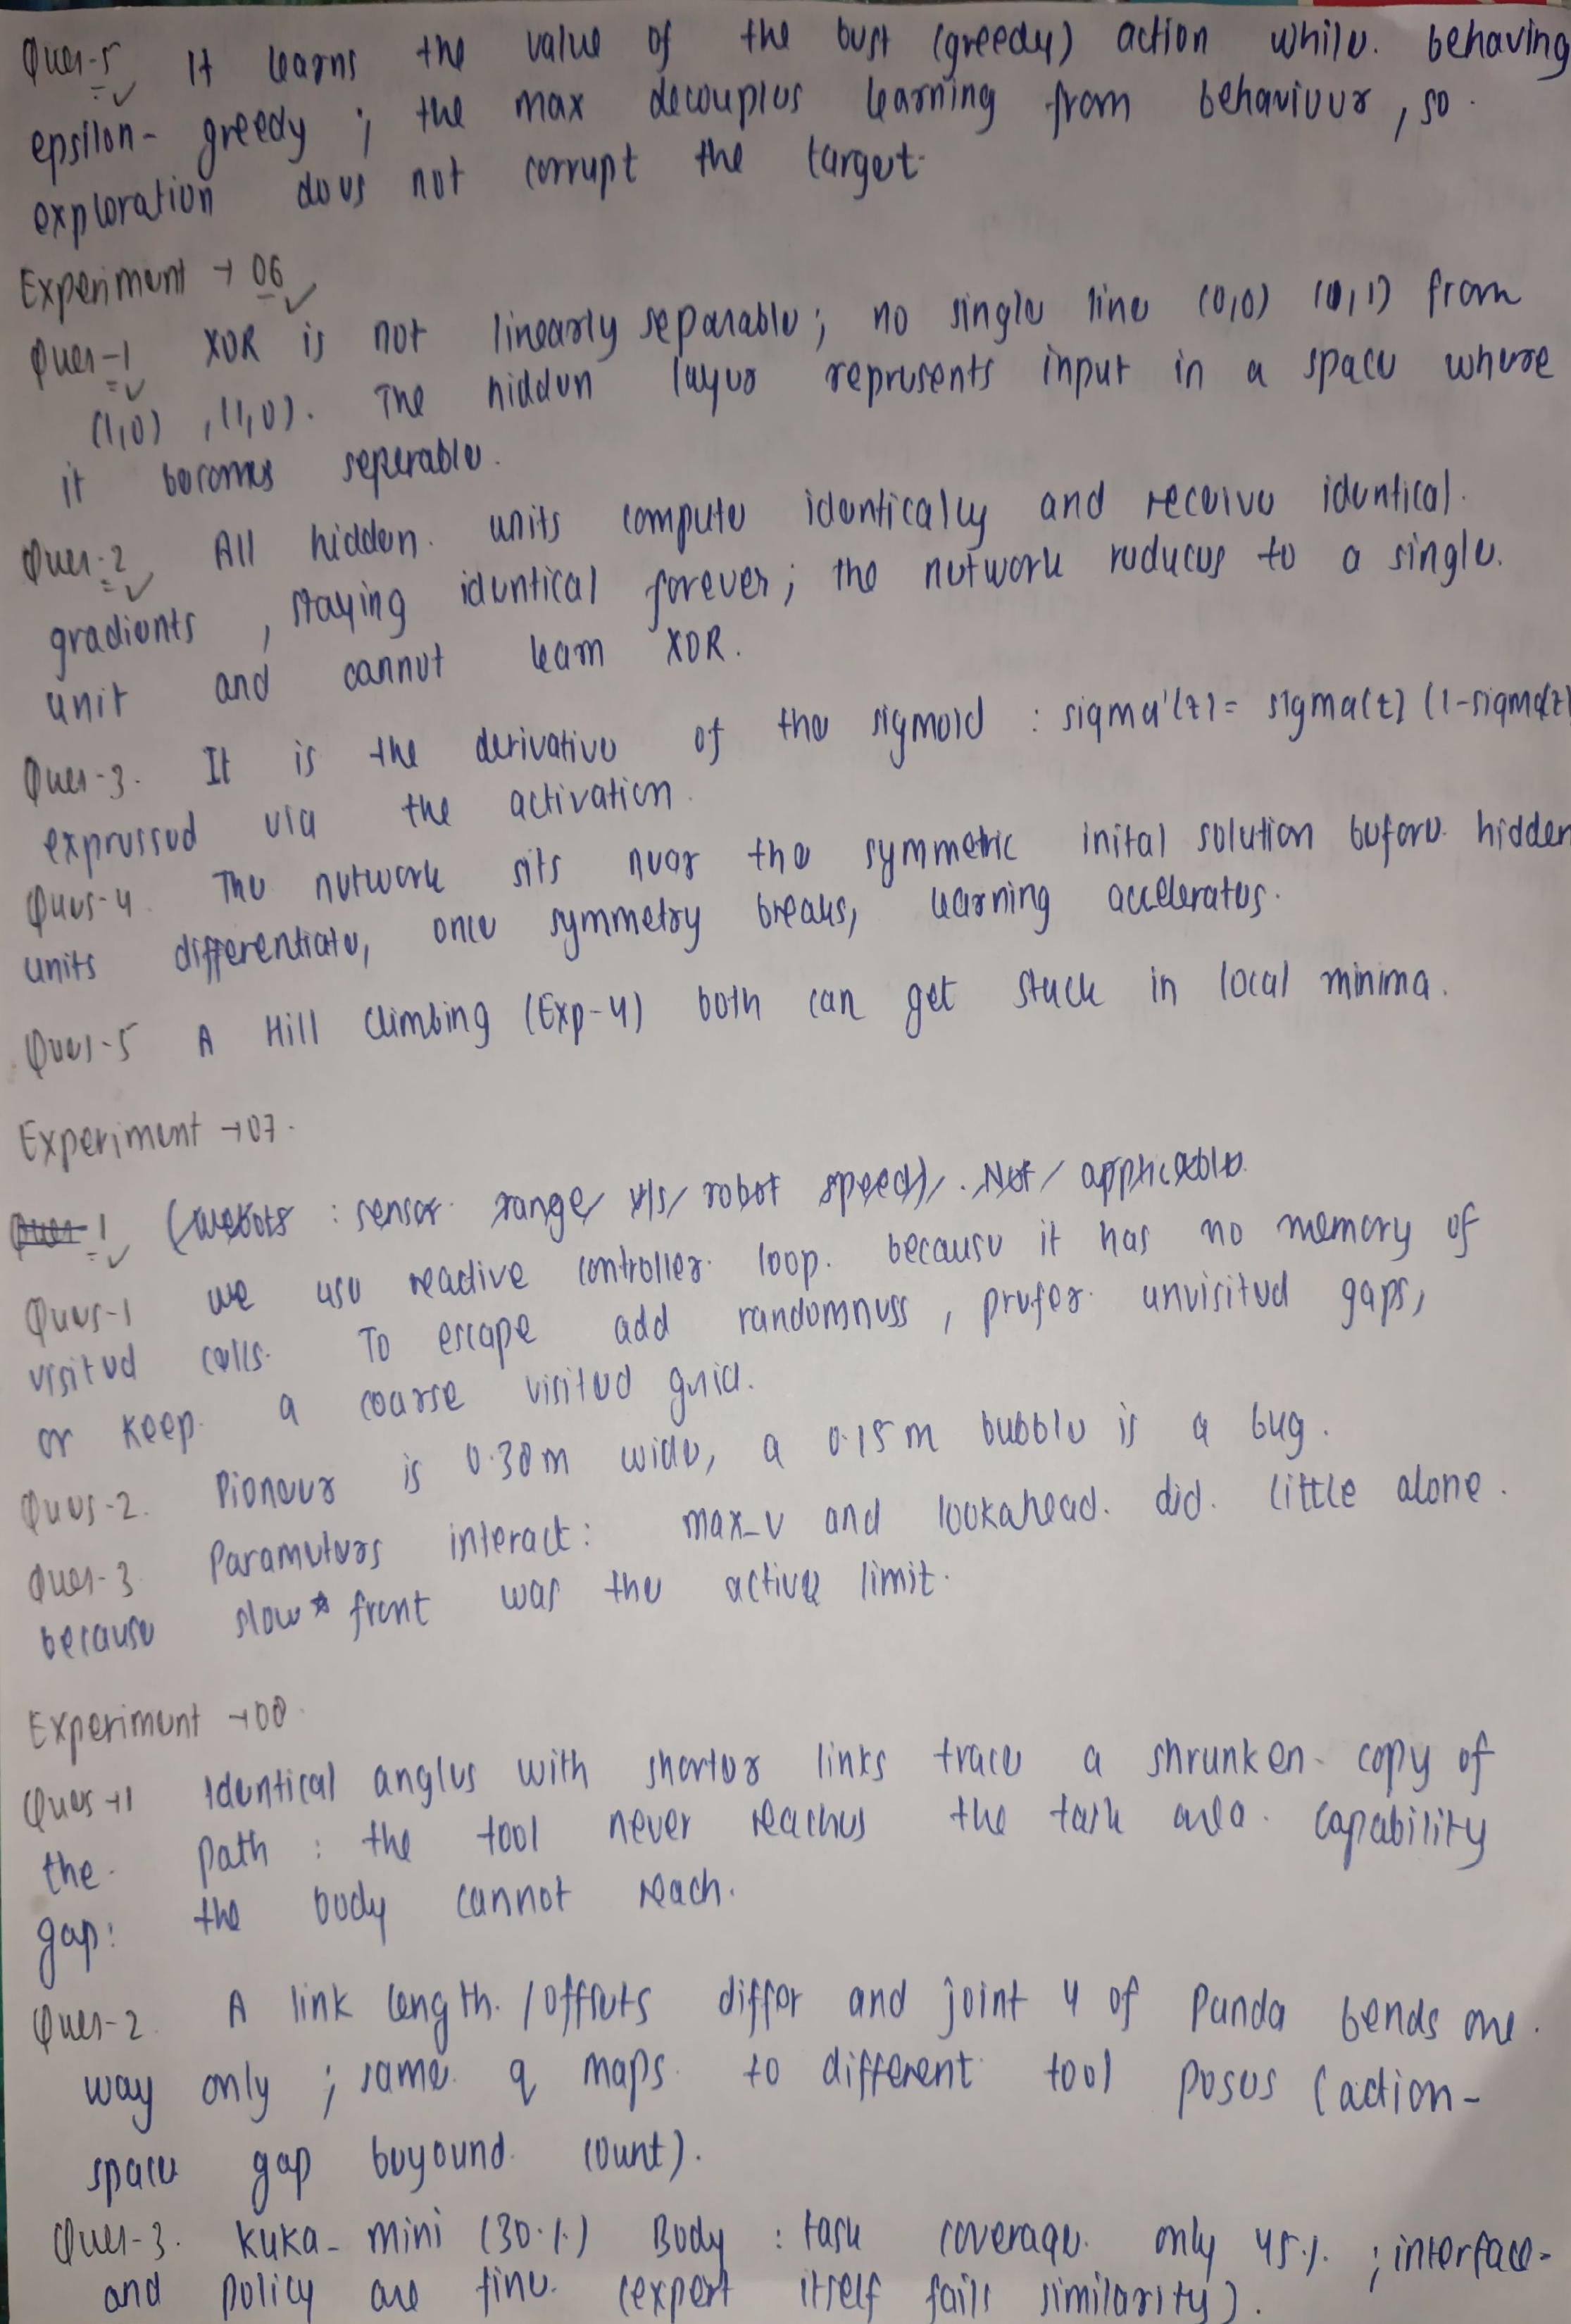
\includegraphics[keepaspectratio,alt={Handwritten answers (scanned) --- page 3}]{handwritten_p3.png}}
\caption{Handwritten answers (scanned) --- page 3}
\end{figure}

\emph{Scanned handwritten answer sheet, page 3, covering this
experiment's Questions section.}

\subsection{6.12 Conclusion}\label{conclusion-5}

The two-layer network learned XOR from random init; learning rate
strongly affected convergence speed, with lr=2.0 fastest and stable on
this tiny problem.

\section{Experiment 7: Webots: Reactive swarm and Lidar
navigation}\label{experiment-7-webots-reactive-swarm-and-lidar-navigation}

\subsection{7.1 Aim}\label{aim-6}

To study reactive control: Braitenberg obstacle avoidance in a
multi-robot swarm and follow-the-gap LiDAR navigation, measuring
coverage, stuck time and safety.

\subsection{7.2 Objectives}\label{objectives-6}

\begin{enumerate}
\def\labelenumi{\arabic{enumi}.}
\tightlist
\item
  Implement and run a Braitenberg vehicle swarm in Webots.
\item
  Measure coverage and stuck percentage vs parameters.
\item
  Implement follow-the-gap navigation with a SICK LMS 291.
\item
  Relate safety bubble size to robot width.
\item
  Explain why reactive controllers loop and how to escape.
\end{enumerate}

\subsection{7.3 Place in the syllabus}\label{place-in-the-syllabus-6}

Unit II/III: reactive vs deliberative control, configuration space.
Contributes to CO1, CO3.

\subsection{7.4 Requirements}\label{requirements-6}

Webots R2025a, Python 3; matplotlib, numpy for plots.

\subsection{7.5 Theory}\label{theory-6}

Braitenberg: sensor readings scaled 0-1 drive wheels via mirror-image
weights; obstacle on right slows left wheel and speeds right wheel
-\textgreater{} turn left. Follow-the-gap: clip scan, mark free beams,
cut safety bubble around closest obstacle, find widest gap, steer to its
middle; speed from front distance. Reactive control has no memory
-\textgreater{} loops.

\subsection{7.6 Method}\label{method-6}

\begin{enumerate}
\def\labelenumi{\arabic{enumi}.}
\tightlist
\item
  Open/run swarm\_arena.wbt; logger records 120 s.
\item
  Run headless with run\_experiment.py; vary parameters.
\item
  Plot trajectories and coverage.
\item
  Run pioneer\_lidar.wbt; vary bubble, k\_turn etc.
\item
  Record metrics.
\end{enumerate}

\subsection{7.7 Procedure and code}\label{procedure-and-code-6}

Run in \texttt{/exp07-webots/code}:
\texttt{python\ tools/run\_experiment.py\ swarm\ -\/-seconds\ 120} and
\texttt{...\ pioneer\ -\/-seconds\ 180}. Code stored under
\texttt{exp07-webots/code}.

\subsection{7.8 Results}\label{results-6}

Table 7.1: Swarm metrics (120 s, 5 e-pucks).

{\def\LTcaptype{none} % do not increment counter
\begin{longtable}[]{@{}llll@{}}
\toprule\noalign{}
Run & Mean path/robot (m) & Worst stuck & Coverage \\
\midrule\noalign{}
\endhead
\bottomrule\noalign{}
\endlastfoot
default (cruise 0.5) & 6.4 & 2.7\% & 75\% \\
cruise = 0.9 & 9.2-10.4 & 75.7\% (one robot wedged) & 89\% \\
cruise = 0.2 & 2.7 & 0.3\% & 55\% \\
gain = 1 & 6.4 & 5.1\% & 77\% \\
gain = 10 & 6.5 & 1.9\% & 82\% \\
speed = 0.5 & 3.4 & 0.5\% & 61\% \\
noise = 0.3 & 6.4 & 2.1\% & 74\% \\
\end{longtable}
}

Our run (default): e-pucks 6.08-6.68 m, stuck 0.5-2.7\%, coverage 75\%.
cruise=0.9: coverage 89\%, e-puck3 stuck 75.7\%.

Table 7.2: Pioneer metrics (180 s).

{\def\LTcaptype{none} % do not increment counter
\begin{longtable}[]{@{}llll@{}}
\toprule\noalign{}
Run & Distance (m) & Stuck & Coverage \\
\midrule\noalign{}
\endhead
\bottomrule\noalign{}
\endlastfoot
default & 83.6 & 0\% & 23\% \\
bubble = 0.15 & 13.4 & 77.4\% & 12\% \\
bubble = 0.9 & 79.8 & 0\% & 24\% \\
k\_turn = 0.5 & 74.3 & 0\% & 29\% \\
stop = 0.8 & 10.9 & 85\% & 11\% \\
\end{longtable}
}

Our runs match: default 83.60 m, 0\% stuck, 23\% coverage; bubble=0.15
13.40 m, 77.4\% stuck, 12\% coverage.

\begin{figure}
\centering
\pandocbounded{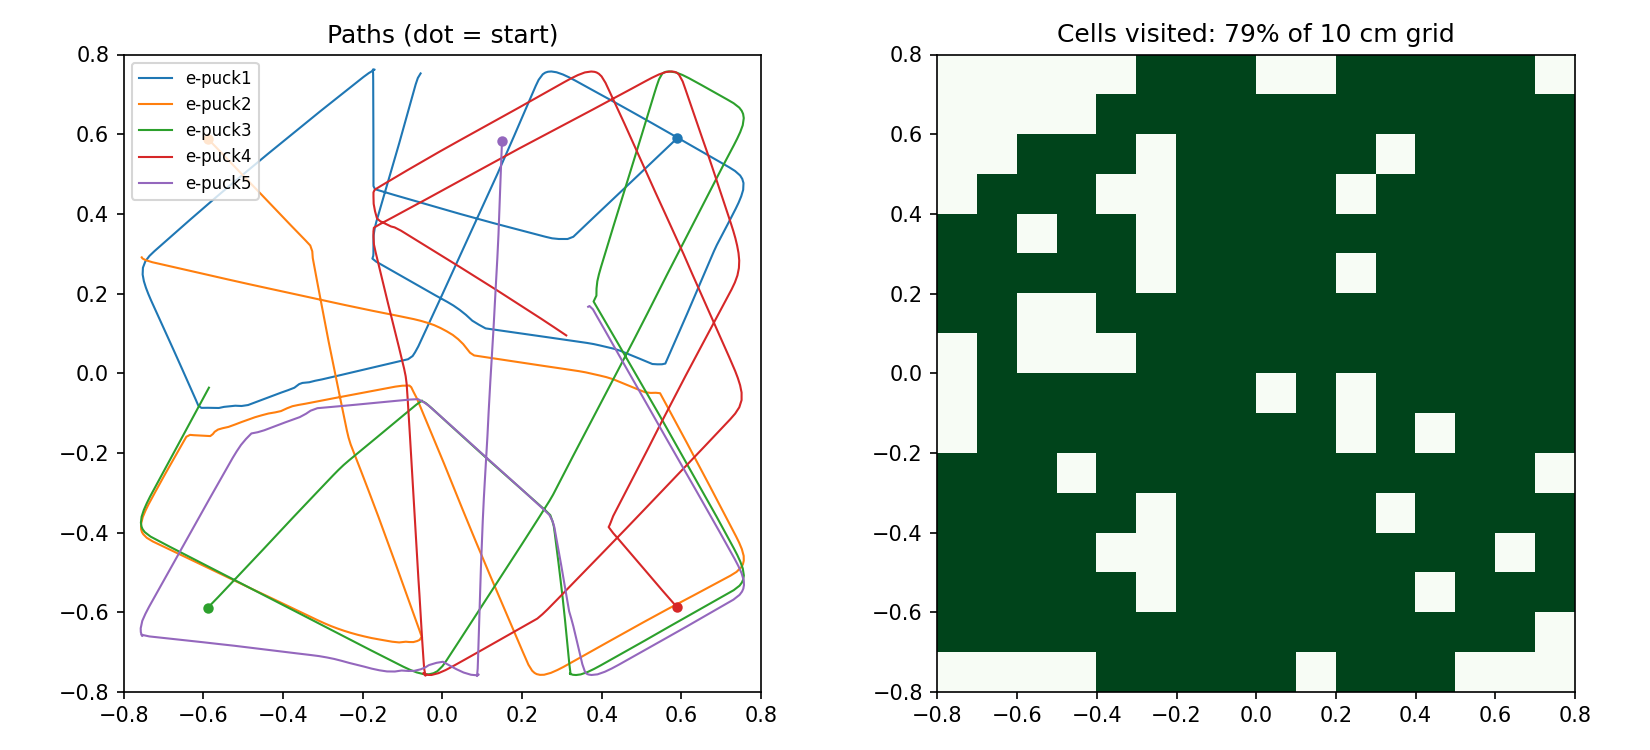
\includegraphics[keepaspectratio,alt={Fig. 7.1 Swarm trajectories and coverage}]{exp07-webots/figs/trajectories.png}}
\caption{Fig. 7.1 Swarm trajectories and coverage}
\end{figure}

\begin{figure}
\centering
\pandocbounded{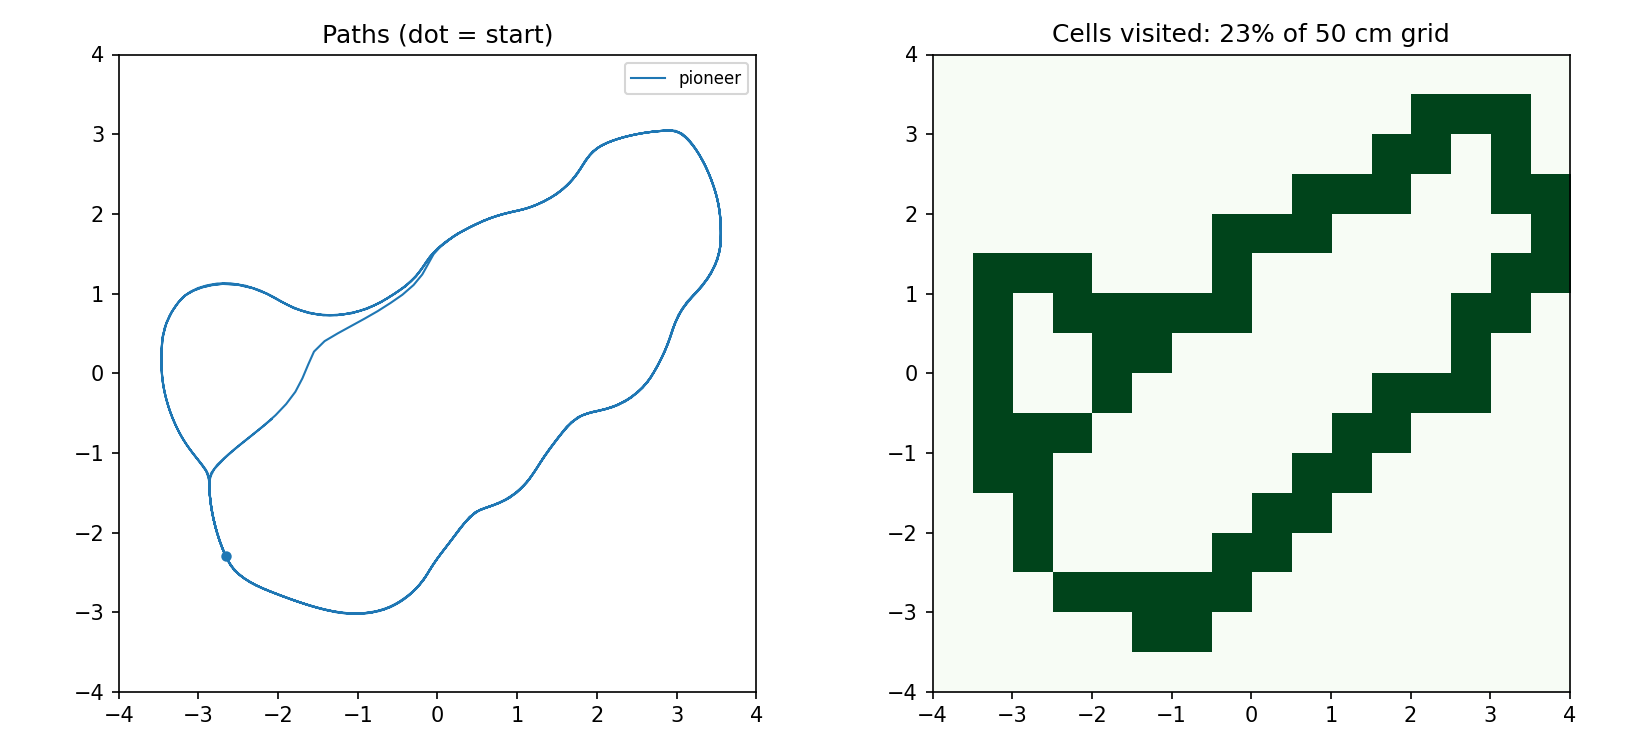
\includegraphics[keepaspectratio,alt={Fig. 7.2 Pioneer default path}]{exp07-webots/figs/pioneer_default.png}}
\caption{Fig. 7.2 Pioneer default path}
\end{figure}

\begin{figure}
\centering
\pandocbounded{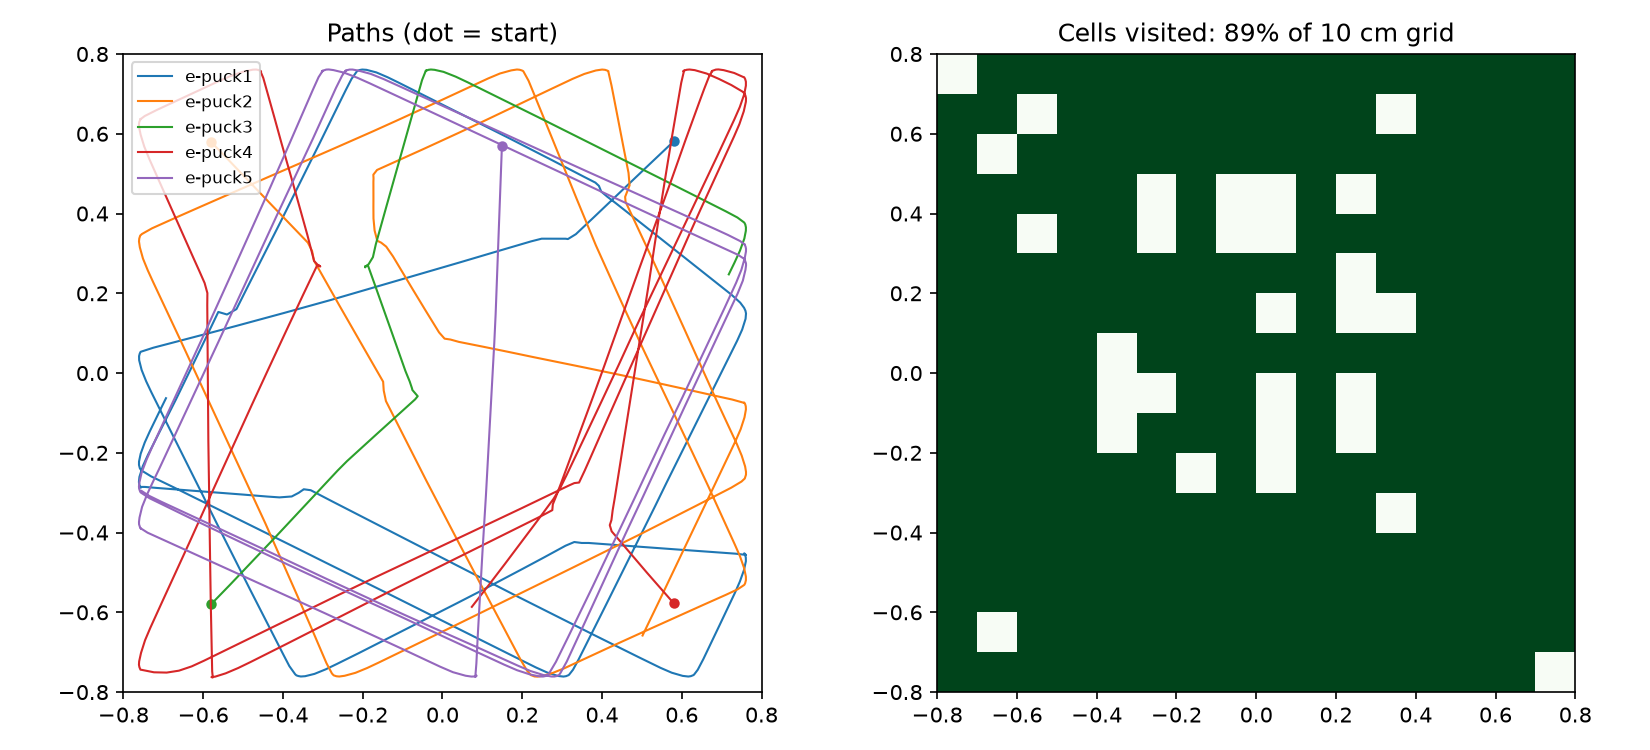
\includegraphics[keepaspectratio,alt={Fig. 7.3 Swarm at cruise 0.9}]{exp07-webots/figs/swarm_cruise-0.9.png}}
\caption{Fig. 7.3 Swarm at cruise 0.9}
\end{figure}

\begin{figure}
\centering
\pandocbounded{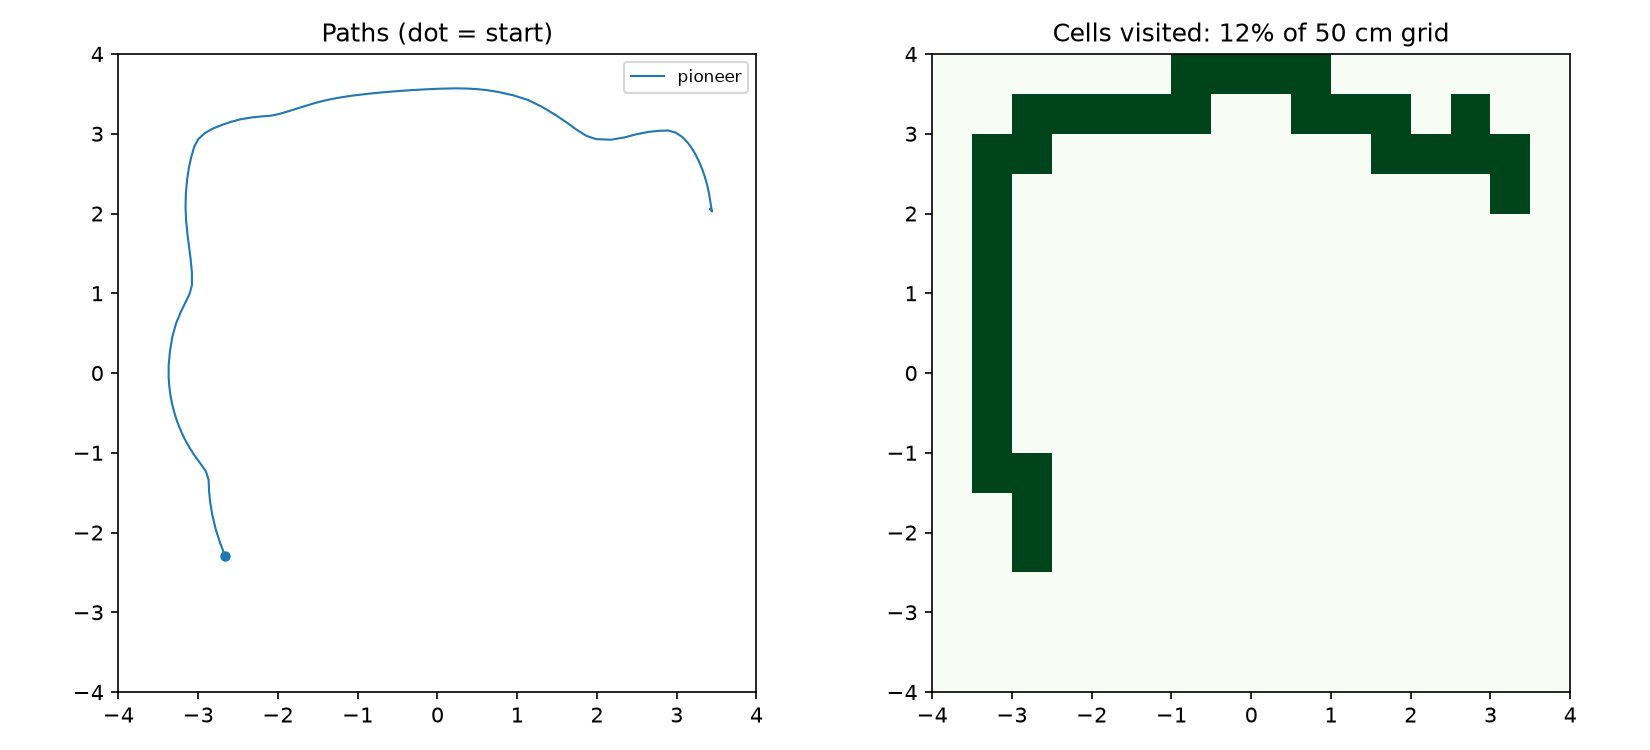
\includegraphics[keepaspectratio,alt={Fig. 7.4 Pioneer bubble 0.15}]{exp07-webots/figs/pioneer_bubble-0.15.png}}
\caption{Fig. 7.4 Pioneer bubble 0.15}
\end{figure}

\subsection{7.9 Observations to record}\label{observations-to-record-6}

Per-run: path m, mean m/s, stuck \%, coverage \%. Parameters changed and
effect.

\subsection{7.10 Applications}\label{applications-6}

Autonomous racing (F1TENTH follow-the-gap), warehouse AGVs, exploration
robots.

\subsection{7.11 Questions and answers}\label{questions-and-answers-6}

Q1. What is an embodiment gap? (Webots: sensor range vs robot speed.)
Not applicable; viva Qs for Webots are from the guide's exercises. Key:
Why does a reactive controller loop? Because it has no memory of visited
cells. How to escape? Add randomness, prefer unvisited gaps, or keep a
coarse visited grid.

Q2. Safety margin must match robot width: Pioneer is 0.38 m wide; a 0.15
m bubble is a bug.

Q3. Parameters interact: max\_v and lookahead did little alone because
slow*front was the active limit.

\begin{figure}
\centering
\pandocbounded{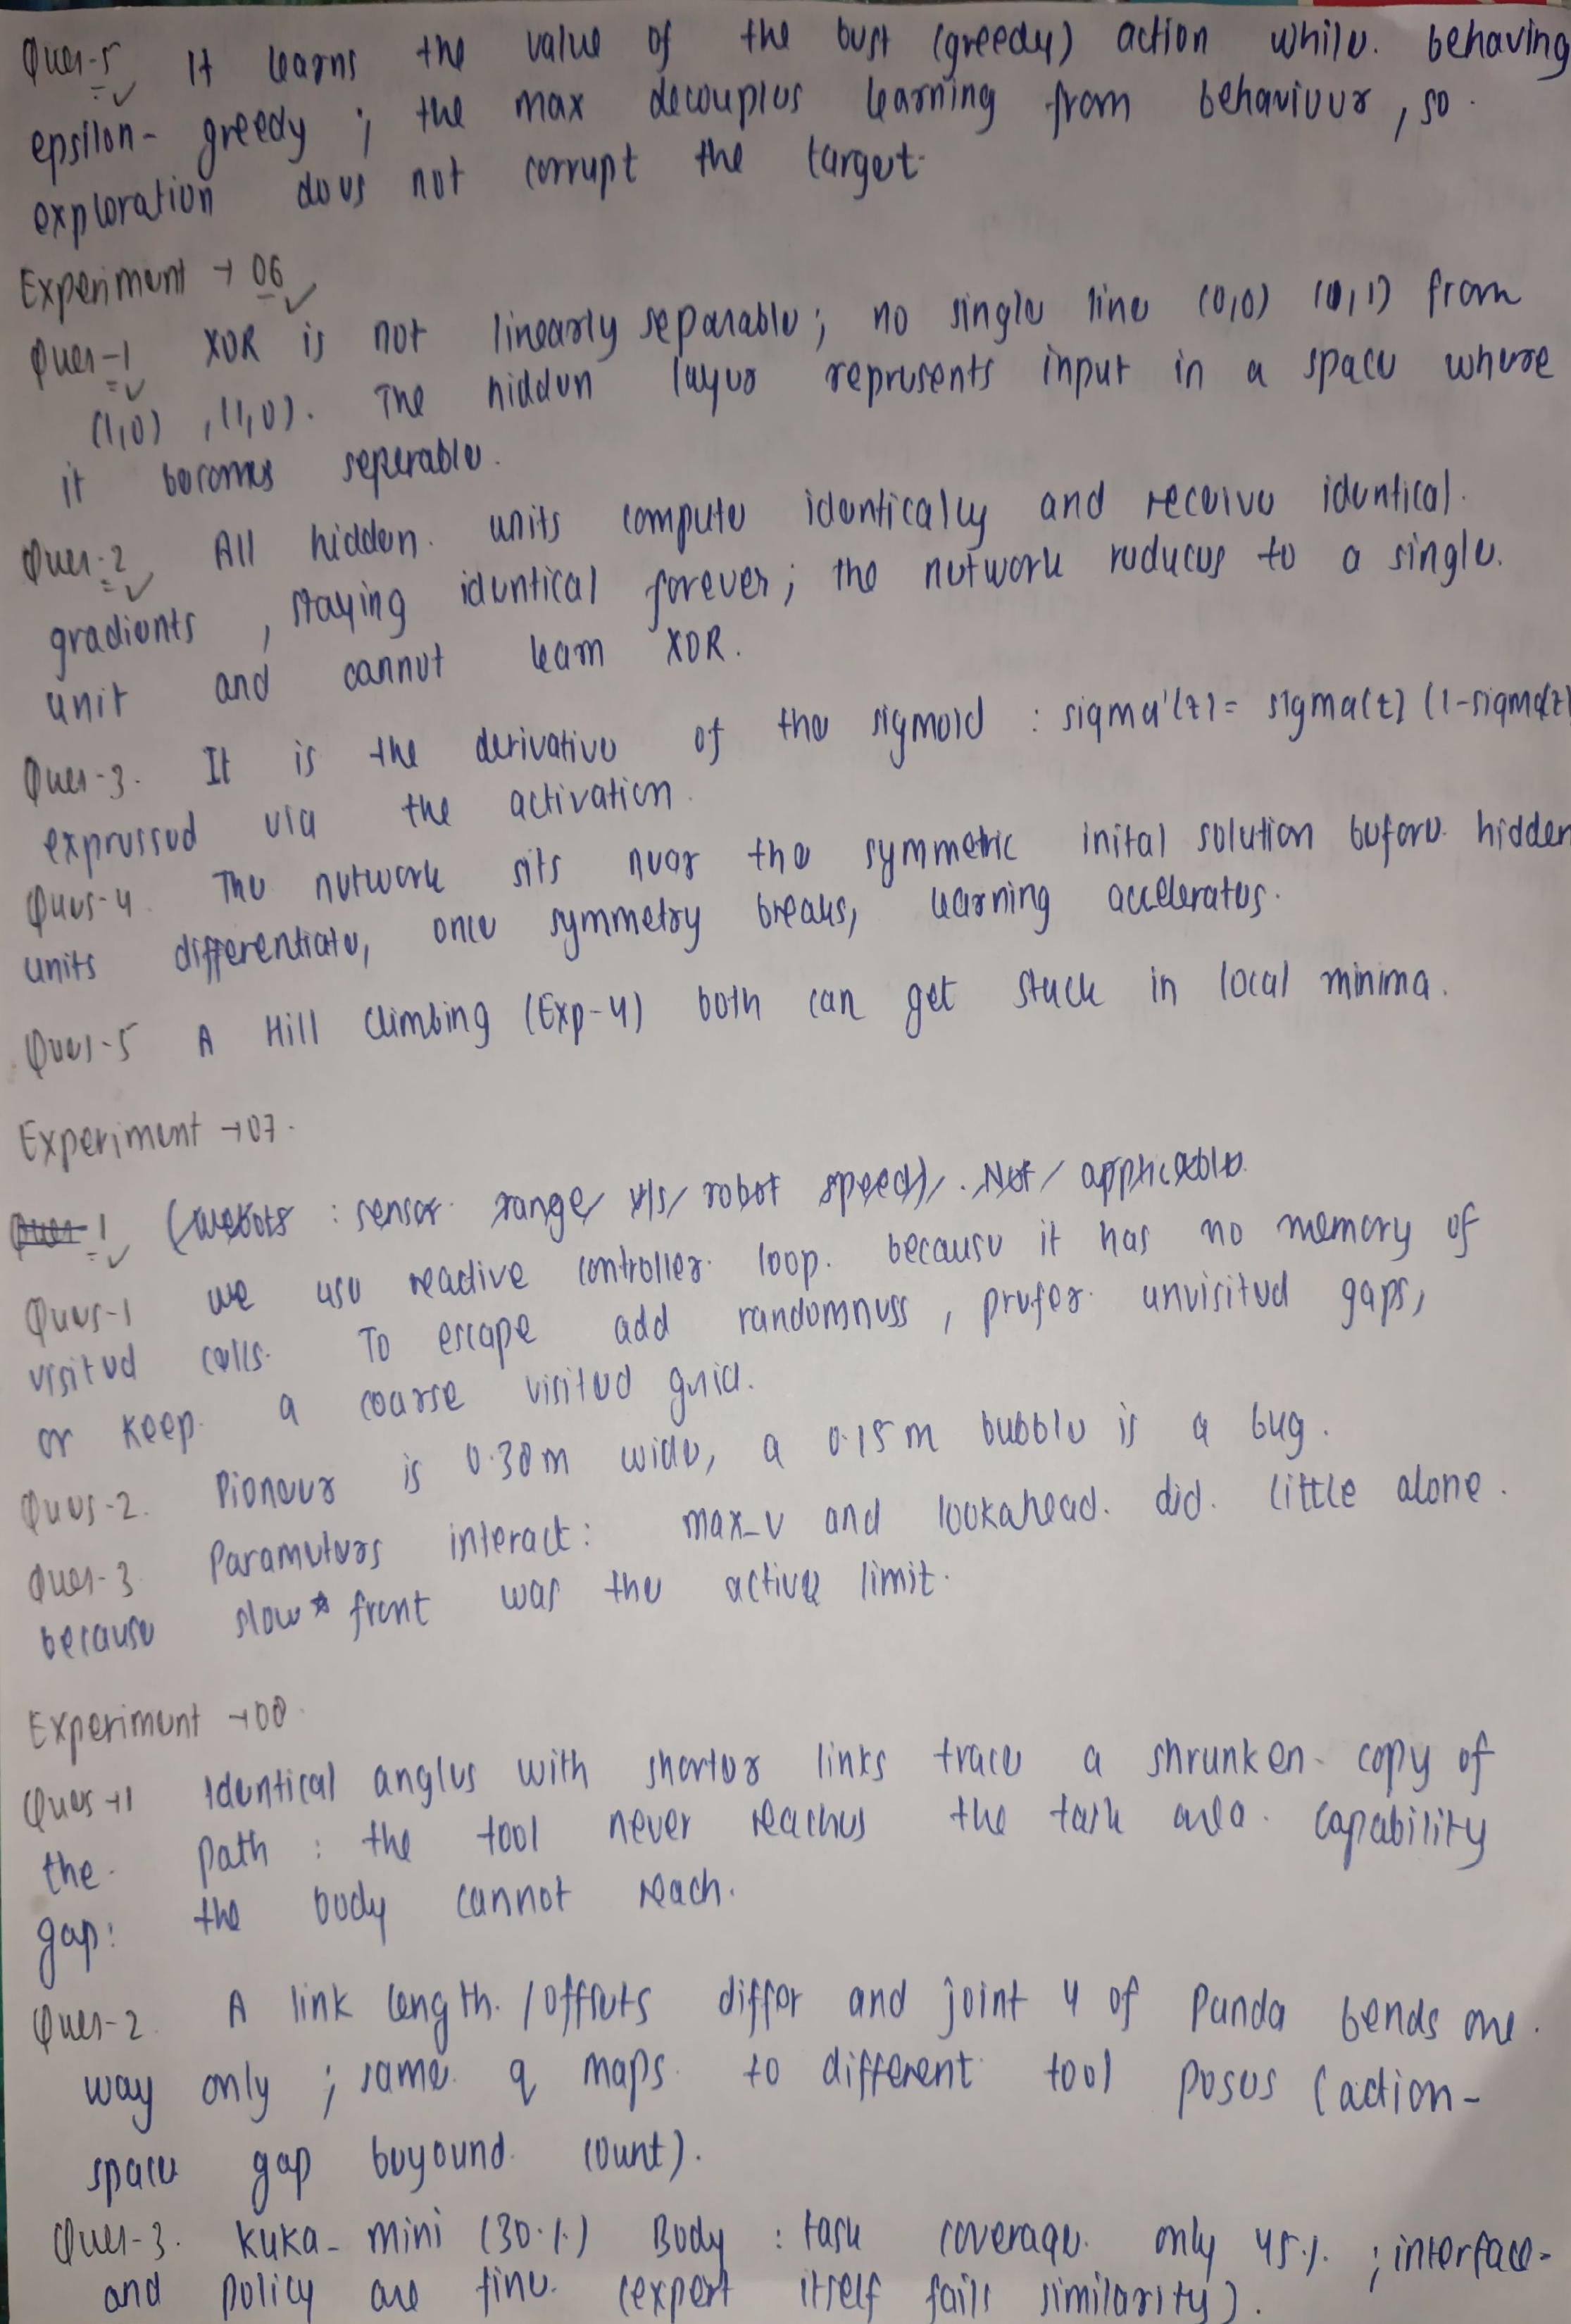
\includegraphics[keepaspectratio,alt={Handwritten answers (scanned) --- page 3}]{handwritten_p3.png}}
\caption{Handwritten answers (scanned) --- page 3}
\end{figure}

\emph{Scanned handwritten answer sheet, page 3, covering this
experiment's Questions section.}

\subsection{7.12 Conclusion}\label{conclusion-6}

Reactive Braitenberg swarm covered 75\% of the arena at default speed
with low stuck time; raising cruise to 0.9 raised coverage to 89\% but
wedged one robot. The Pioneer never collided but looped, covering only
23\%; a too-small safety bubble caused 77\% stuck time.

\section{Experiment 8: Cross-embodiment transfer in
PyBullet}\label{experiment-8-cross-embodiment-transfer-in-pybullet}

\subsection{8.1 Aim}\label{aim-7}

To study whether a pick-and-place skill developed on one robot arm
transfers to arms with different kinematics, joint counts and sizes, and
to identify which design choices make transfer succeed or fail.

\subsection{8.2 Objectives}\label{objectives-7}

\begin{enumerate}
\def\labelenumi{\arabic{enumi}.}
\tightlist
\item
  Describe embodiment via measurable quantities (DOF, limits, reach,
  workspace).
\item
  Explain why copying joint angles does not transfer.
\item
  Use shared task-space action space and IK adapter.
\item
  Train behaviour-cloning policy and test zero-shot on unseen robots.
\item
  Explain observation choice (task-space vs joint angles) effect.
\item
  Separate interface problem from capability problem.
\end{enumerate}

\subsection{8.3 Place in the syllabus}\label{place-in-the-syllabus-7}

Unit II/III: kinematics, configuration space, planning. Contributes to
CO1, CO3.

\subsection{8.4 Requirements}\label{requirements-7}

Python 3.10/3.11, PyBullet, NumPy, Matplotlib, scikit-learn. See
\texttt{exp08-xembody/code}.

\subsection{8.5 Theory}\label{theory-7}

Embodiment: DOF, link lengths, limits, gripper, mount. Embodiment gap:
action-space, observation, dynamics, capability. Joint space vs task
space: same q gives different poses; same desired x can be sent to any
robot with IK. Shared interface: obs = {[}tool xyz, holding, cube xyz,
goal xyz{]} (10), action = {[}dx,dy,dz,grip{]} (4). BC on (obs, expert
action) pairs; DART noise injection. Multi-embodiment training.

\subsection{8.6 Method}\label{method-7}

Parts 0-5 per manual: setup check, measure bodies, joint-space replay,
task-space transfer, learn on KUKA deploy on all,
leave-one-embodiment-out.

\subsection{8.7 Procedure and code}\label{procedure-and-code-7}

Run in \texttt{exp08-xembody/code}: experiments 00..05. Code stored
under \texttt{exp08-xembody/code}.

\subsection{8.8 Results}\label{results-7}

Table 8.1: Embodiments.

{\def\LTcaptype{none} % do not increment counter
\begin{longtable}[]{@{}llll@{}}
\toprule\noalign{}
Robot & Arm DOF & Max reach (m) & Task coverage \\
\midrule\noalign{}
\endhead
\bottomrule\noalign{}
\endlastfoot
kuka\_iiwa & 7 & 0.945 & 100\% \\
franka\_panda & 7 & 0.944 & 100\% \\
xarm6 & 6 & 0.759 & 100\% \\
kuka\_mini & 7 & 0.662 & 47.8\% \\
\end{longtable}
}

Table 8.2: Joint-space replay of KUKA trajectories (10 episodes).

{\def\LTcaptype{none} % do not increment counter
\begin{longtable}[]{@{}llll@{}}
\toprule\noalign{}
Robot & Success & Mean path dev (cm) & Median cube-goal err (cm) \\
\midrule\noalign{}
\endhead
\bottomrule\noalign{}
\endlastfoot
kuka\_iiwa & 100\% & 1.42 & 0.05 \\
franka\_panda & 0\% & 16.7 & 29.2 \\
xarm6 & 0\% & 27.2 & 34.3 \\
kuka\_mini & 0\% & 17.6 & 34.3 \\
\end{longtable}
}

Table 8.3: Task-space transfer of expert (20 episodes).

{\def\LTcaptype{none} % do not increment counter
\begin{longtable}[]{@{}llll@{}}
\toprule\noalign{}
Robot & Success & Mean steps & Median cube-goal err (cm) \\
\midrule\noalign{}
\endhead
\bottomrule\noalign{}
\endlastfoot
kuka\_iiwa & 100\% & 50.5 & 0.15 \\
franka\_panda & 100\% & 46.6 & 0.13 \\
xarm6 & 100\% & 44.9 & 0.27 \\
kuka\_mini & 30\% & 43.8 & 1.54 \\
\end{longtable}
}

Table 8.4: Learn on KUKA, deploy everywhere (60 demos, 20 test
episodes).

{\def\LTcaptype{none} % do not increment counter
\begin{longtable}[]{@{}llll@{}}
\toprule\noalign{}
Robot & Expert & BC-agnostic & BC-proprio \\
\midrule\noalign{}
\endhead
\bottomrule\noalign{}
\endlastfoot
kuka\_iiwa & 100\% & 100\% & 100\% \\
franka\_panda & 100\% & 100\% & 0\% \\
xarm6 & 100\% & 100\% & 0\% \\
kuka\_mini & 50\% & 55\% & 0\% \\
\end{longtable}
}

Table 8.5: Leave-one-embodiment-out (60 demos per policy).

{\def\LTcaptype{none} % do not increment counter
\begin{longtable}[]{@{}
  >{\raggedright\arraybackslash}p{(\linewidth - 8\tabcolsep) * \real{0.2000}}
  >{\raggedright\arraybackslash}p{(\linewidth - 8\tabcolsep) * \real{0.2000}}
  >{\raggedright\arraybackslash}p{(\linewidth - 8\tabcolsep) * \real{0.2000}}
  >{\raggedright\arraybackslash}p{(\linewidth - 8\tabcolsep) * \real{0.2000}}
  >{\raggedright\arraybackslash}p{(\linewidth - 8\tabcolsep) * \real{0.2000}}@{}}
\toprule\noalign{}
\begin{minipage}[b]{\linewidth}\raggedright
Unseen robot
\end{minipage} & \begin{minipage}[b]{\linewidth}\raggedright
single, agnostic
\end{minipage} & \begin{minipage}[b]{\linewidth}\raggedright
multi, agnostic
\end{minipage} & \begin{minipage}[b]{\linewidth}\raggedright
single, proprio
\end{minipage} & \begin{minipage}[b]{\linewidth}\raggedright
multi, proprio
\end{minipage} \\
\midrule\noalign{}
\endhead
\bottomrule\noalign{}
\endlastfoot
kuka\_iiwa & 100\% & 100\% & 0\% & 0\% \\
franka\_panda & 100\% & 100\% & 0\% & 5\% \\
xarm6 & 100\% & 100\% & 0\% & 0\% \\
\end{longtable}
}

\begin{figure}
\centering
\pandocbounded{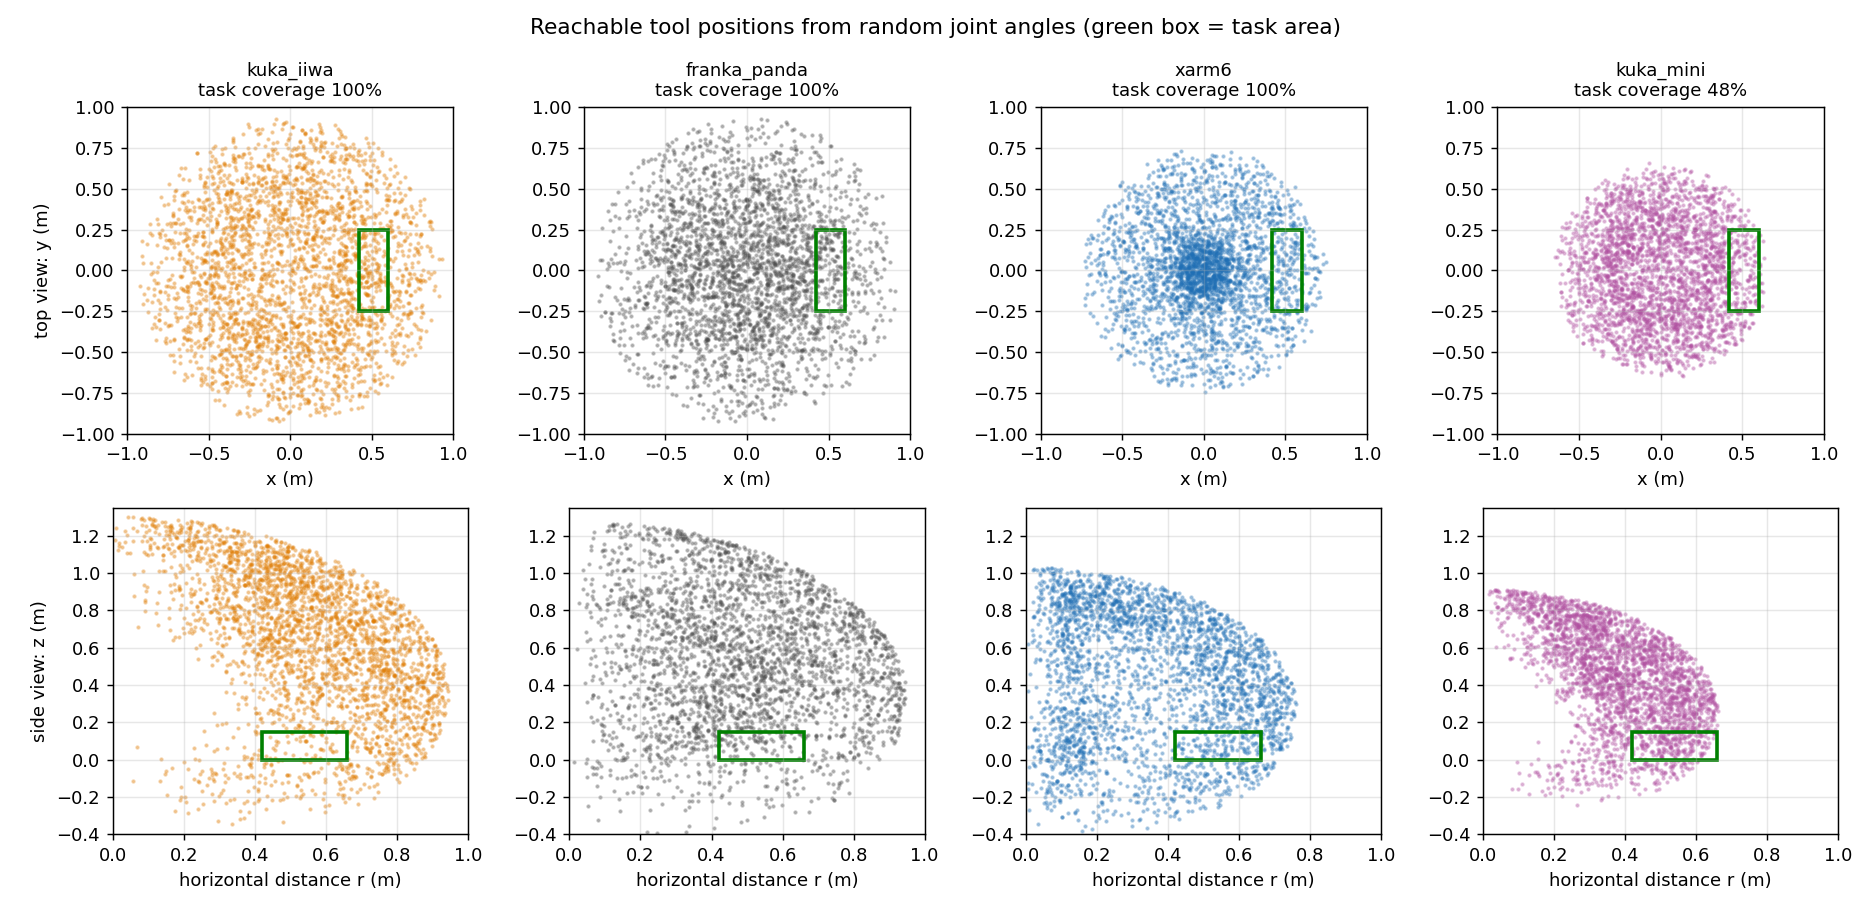
\includegraphics[keepaspectratio,alt={Fig. 8.1 Workspace}]{exp08-xembody/code/results/01_workspace.png}}
\caption{Fig. 8.1 Workspace}
\end{figure}

\begin{figure}
\centering
\pandocbounded{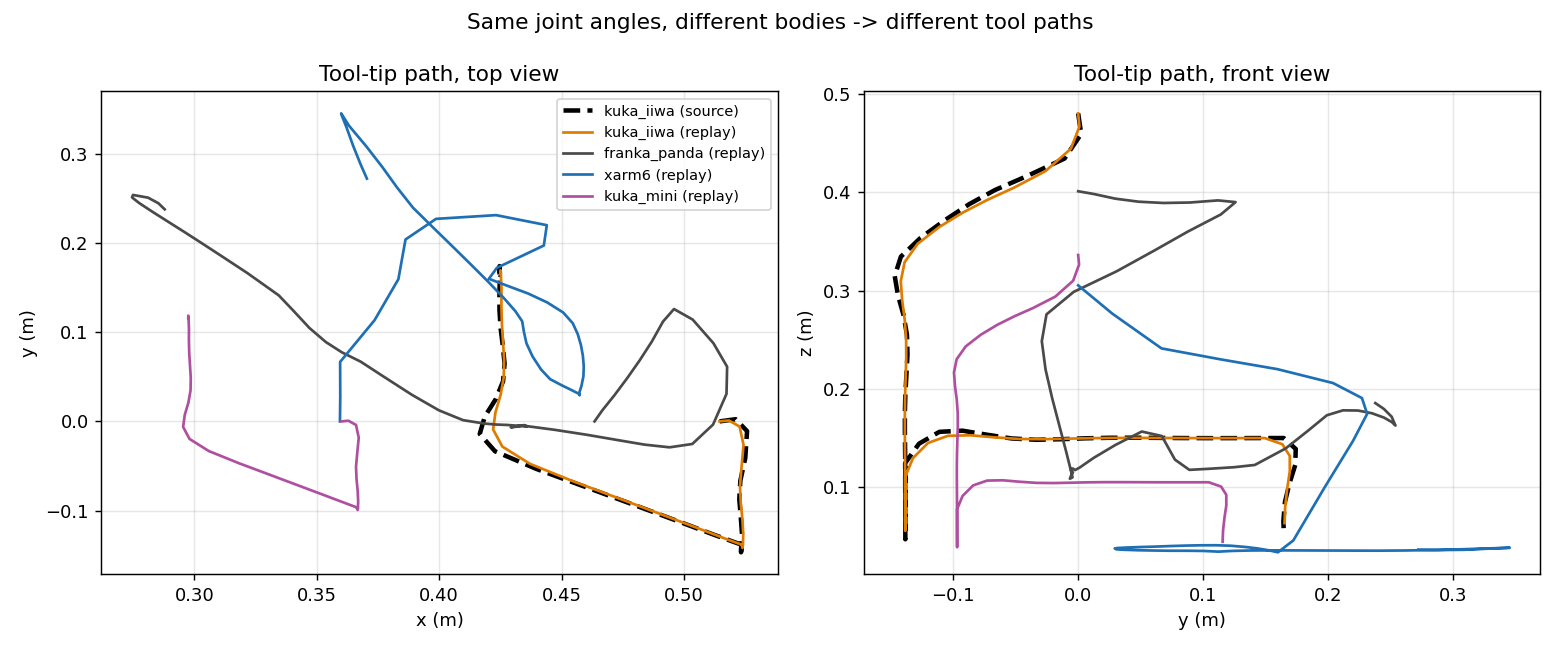
\includegraphics[keepaspectratio,alt={Fig. 8.2 Joint-space replay paths}]{exp08-xembody/code/results/02_joint_space_paths.png}}
\caption{Fig. 8.2 Joint-space replay paths}
\end{figure}

\begin{figure}
\centering
\pandocbounded{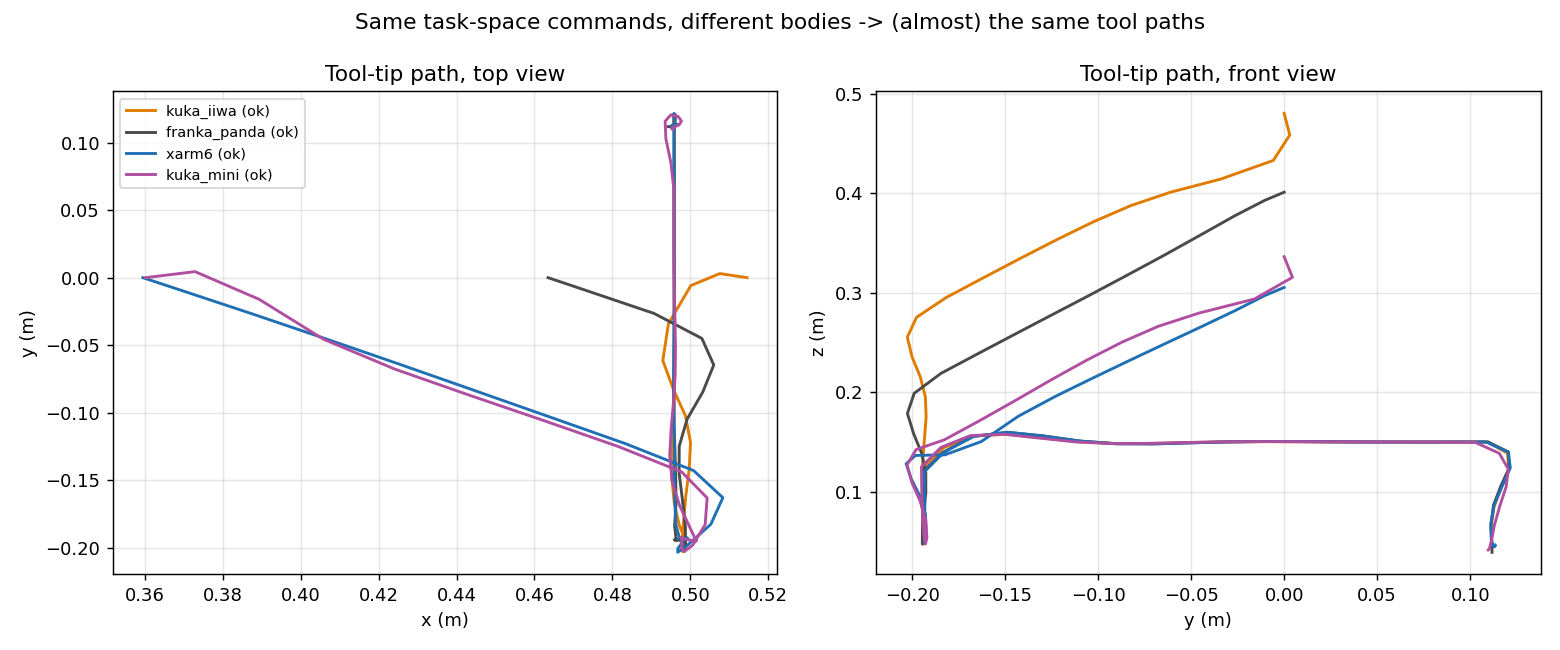
\includegraphics[keepaspectratio,alt={Fig. 8.3 Task-space transfer paths}]{exp08-xembody/code/results/03_task_space_paths.png}}
\caption{Fig. 8.3 Task-space transfer paths}
\end{figure}

\begin{figure}
\centering
\pandocbounded{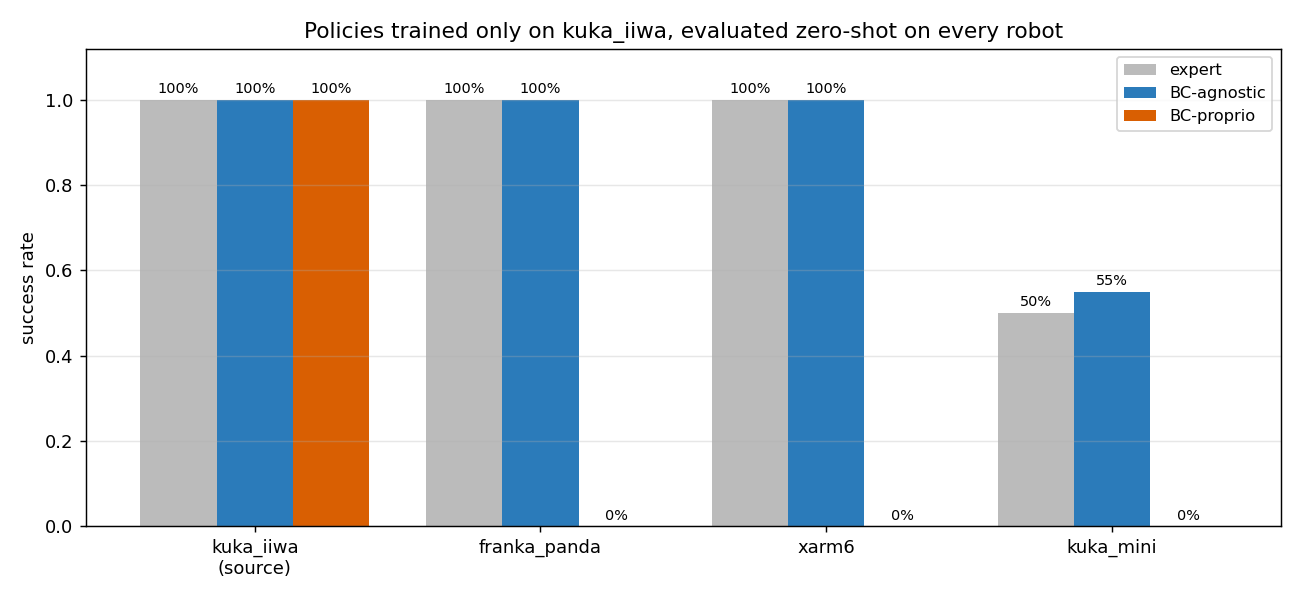
\includegraphics[keepaspectratio,alt={Fig. 8.4 Learn once deploy many}]{exp08-xembody/code/results/04_learn_once_deploy_many_kuka_iiwa.png}}
\caption{Fig. 8.4 Learn once deploy many}
\end{figure}

\begin{figure}
\centering
\pandocbounded{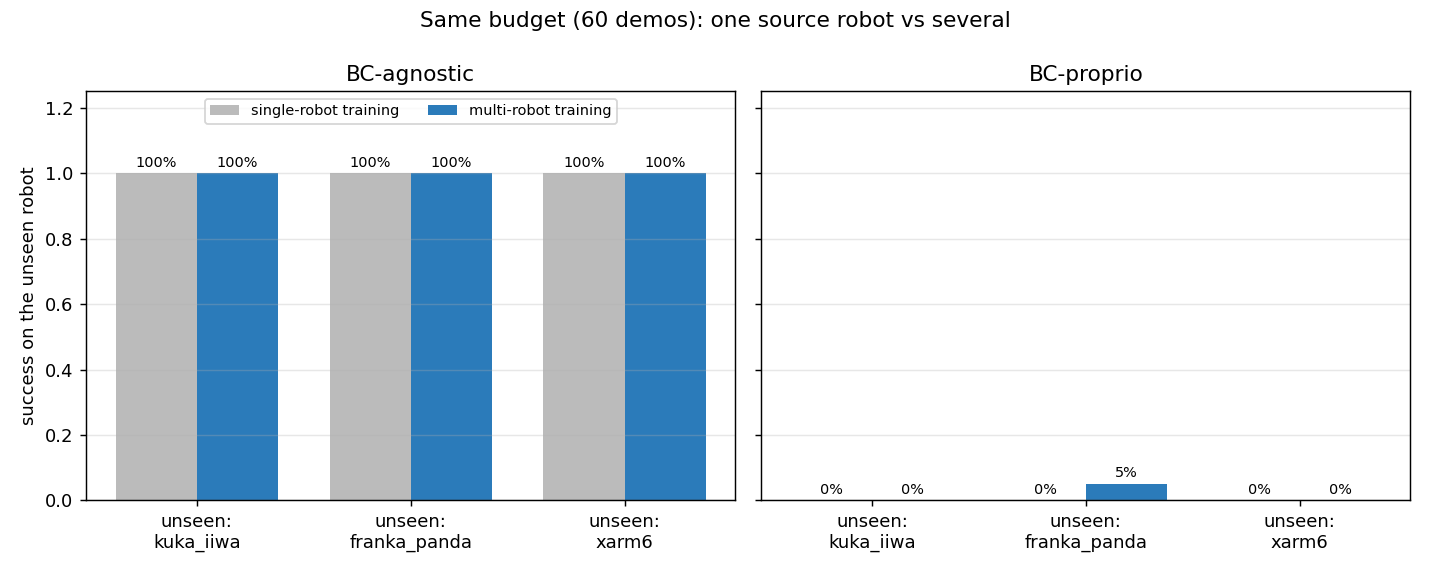
\includegraphics[keepaspectratio,alt={Fig. 8.5 Multi-embodiment training}]{exp08-xembody/code/results/05_multi_embodiment.png}}
\caption{Fig. 8.5 Multi-embodiment training}
\end{figure}

\subsection{8.9 Observations to record}\label{observations-to-record-7}

DOF, max reach, task coverage; joint-space replay metrics; task-space
transfer metrics; BC success rates; leave-one-out success rates.

\subsection{8.10 Applications}\label{applications-7}

Cross-embodiment datasets (Open X-Embodiment), RT-X/Octo/CrossFormer/HPT
generalist policies.

\subsection{8.11 Questions and answers}\label{questions-and-answers-7}

Q1. Why does joint-space replay fail on kuka\_mini, which has the same
joints and angles? A: Identical angles with shorter links trace a
shrunken copy of the path; the tool never reaches the task area.
Capability gap: the body cannot reach.

Q2. Panda and KUKA both have 7 joints. Why is same DOF not enough? A:
Link lengths/offsets differ and joint 4 of Panda bends one way only;
same q maps to different tool poses (action-space gap beyond count).

Q3. In task-space transfer, which robot still fails, and is it
interface, policy or body? A: kuka\_mini (30\%). Body: task coverage
only 48\%; interface and policy are fine (expert itself fails
similarly).

Q4. In Part 4, BC-agnostic vs BC-proprio trained on identical data;
explain difference on other robots via observation gap. A: BC-proprio
includes joint angles, which are body-specific; the policy depends on
the source body and fails to transfer. BC-agnostic uses only task-space
features, so it transfers.

Q5. On kuka\_mini, BC-agnostic and expert score almost the same. Why is
body, not policy, the limit? Why can they still differ by an episode? A:
Both are limited by reach; near the reachable boundary a slightly
different path decides success, so 55\% vs 50\%.

Q6. In Part 5, does multi-embodiment training help BC-proprio? Does it
matter for BC-agnostic? Why? A: Multi training does not rescue
BC-proprio (0-5\%): two bodies too few to learn to ignore joint angles.
BC-agnostic already transfers from one body; multi mainly reduces
placement error.

Q7. Suction gripper hides gripper differences. Name two things that make
a real two-finger gripper harder to transfer. A: Grasp pose/orientation
dependence and gripper-specific contact dynamics/friction.

Q8. Suggest one way to make kuka\_mini succeed without changing the
policy. A: Move its base closer to the task (e.g.~base\_pos=(0.15,0,0))
or scale it up, increasing reach.

\begin{figure}
\centering
\pandocbounded{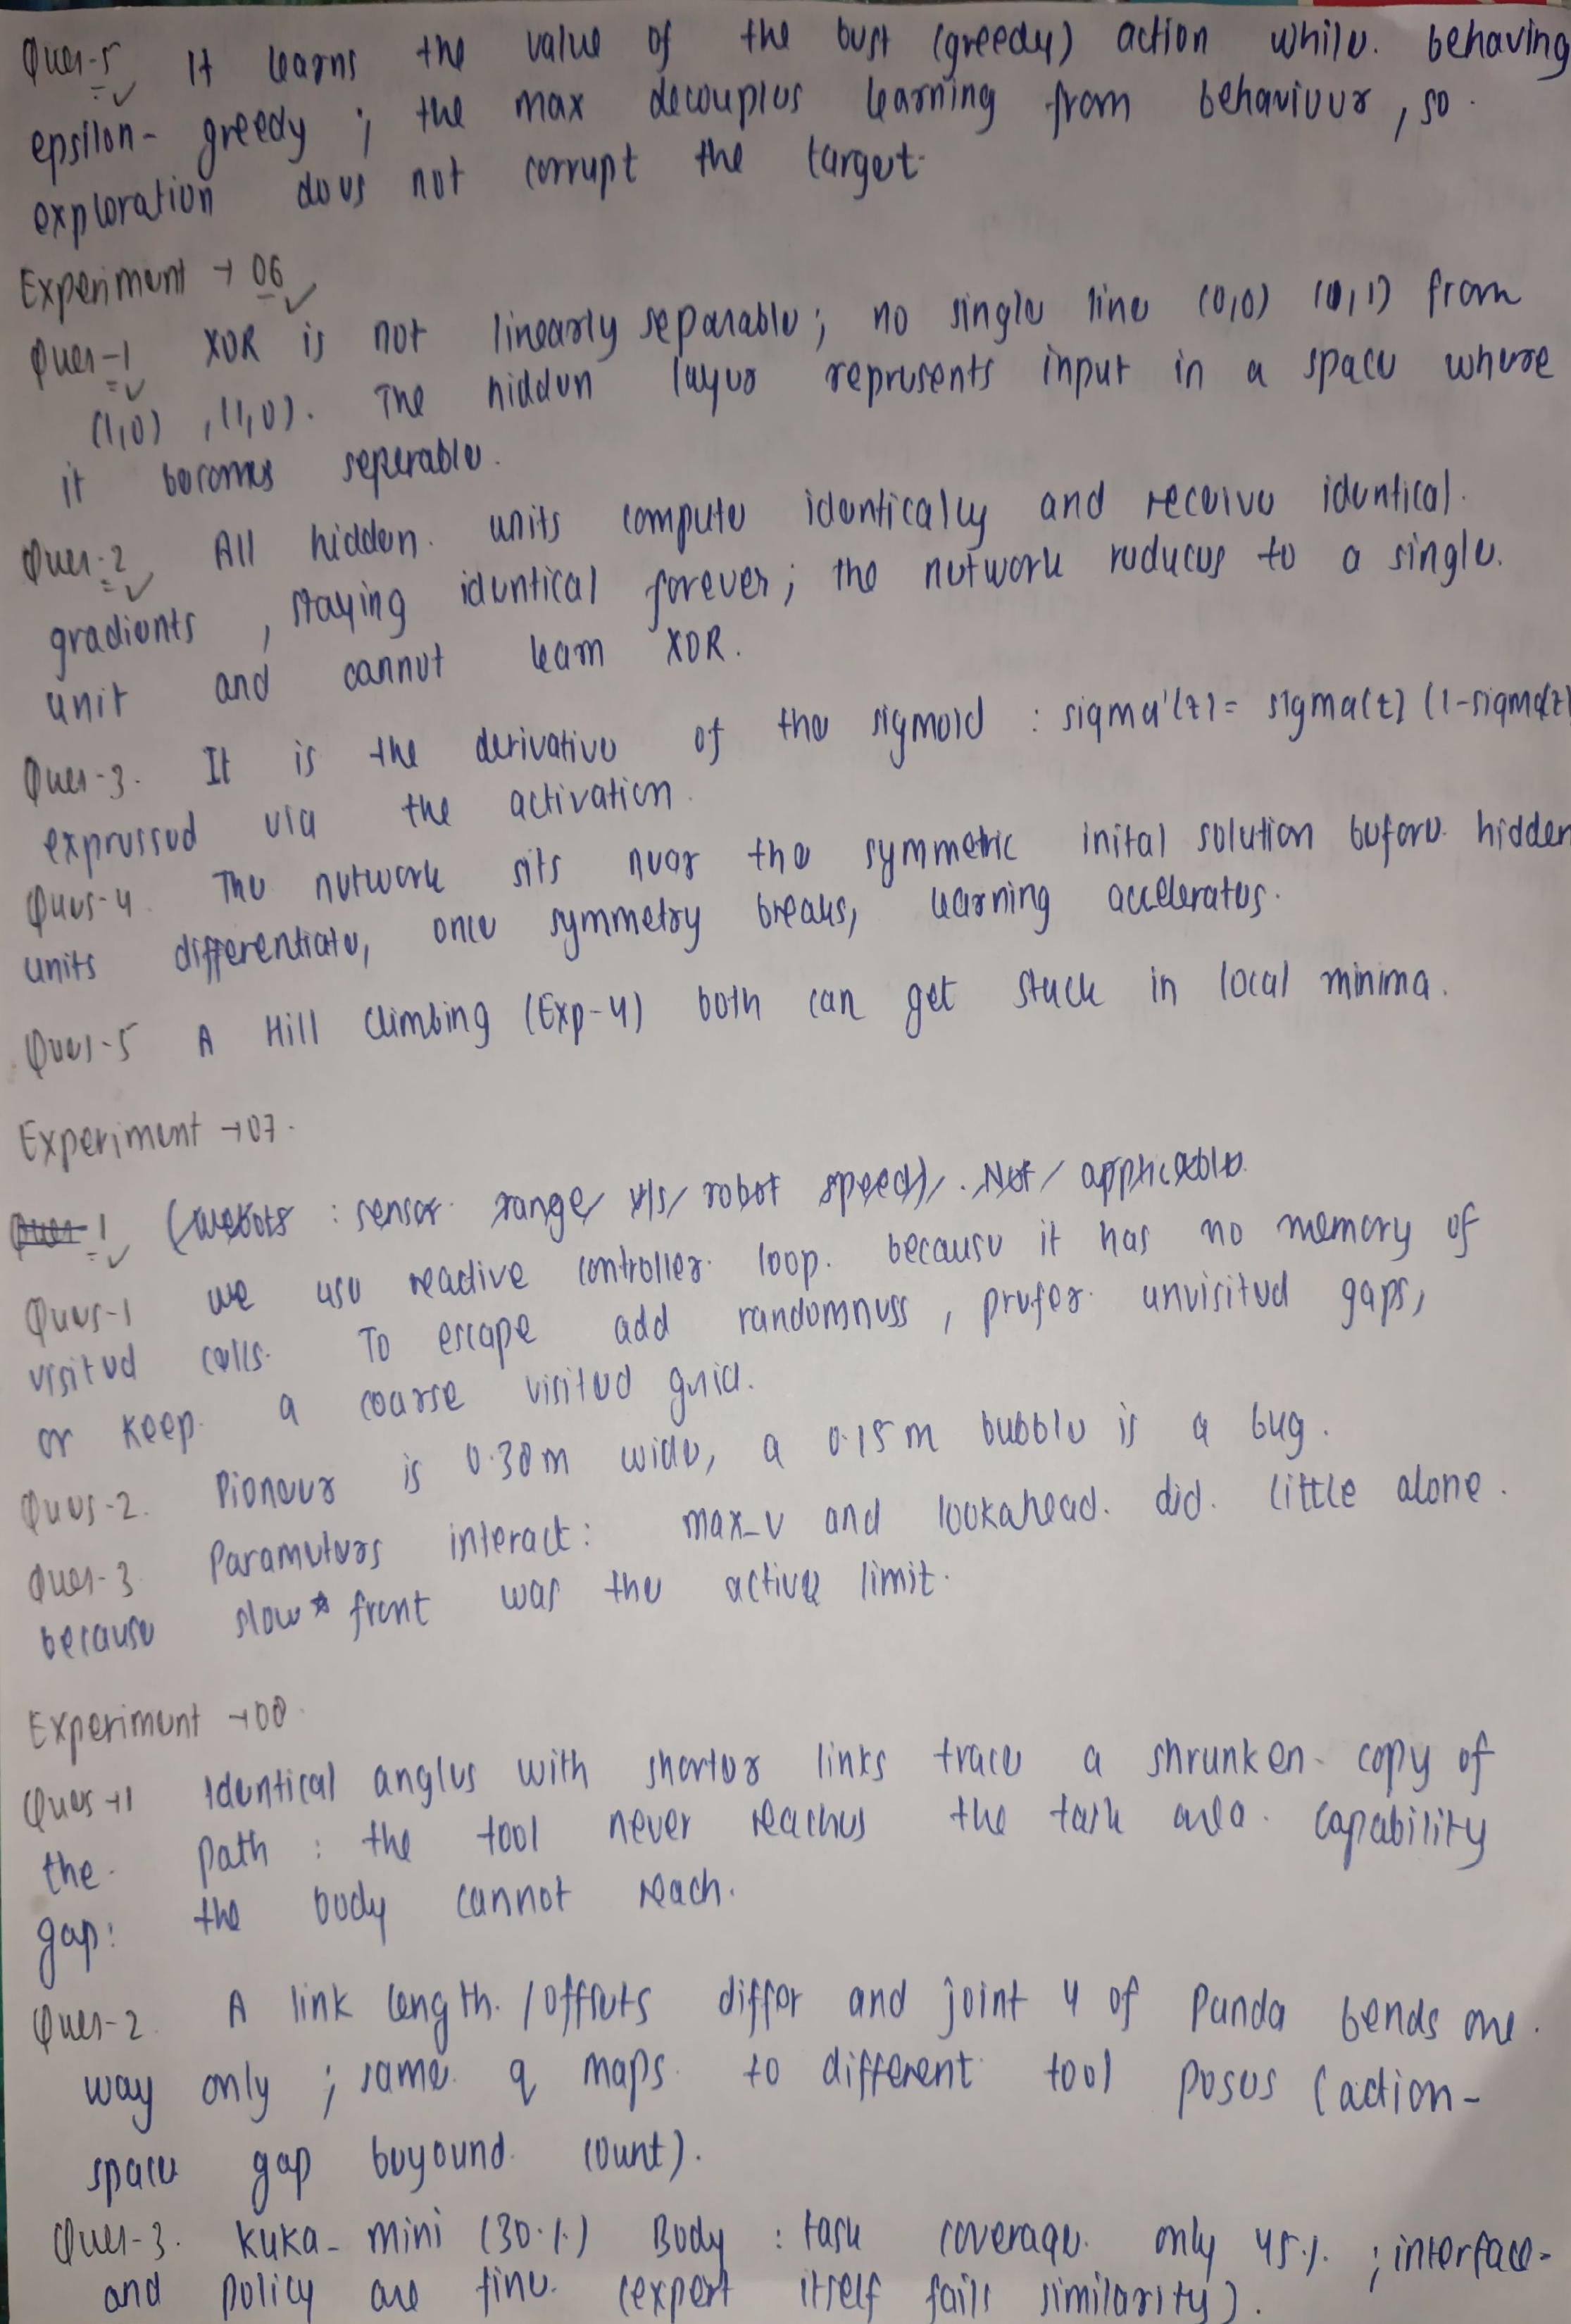
\includegraphics[keepaspectratio,alt={Handwritten answers (scanned) --- page 3}]{handwritten_p3.png}}
\caption{Handwritten answers (scanned) --- page 3}
\end{figure}

\emph{Scanned handwritten answer sheet, page 3, covering this
experiment's Questions section.}

\begin{figure}
\centering
\pandocbounded{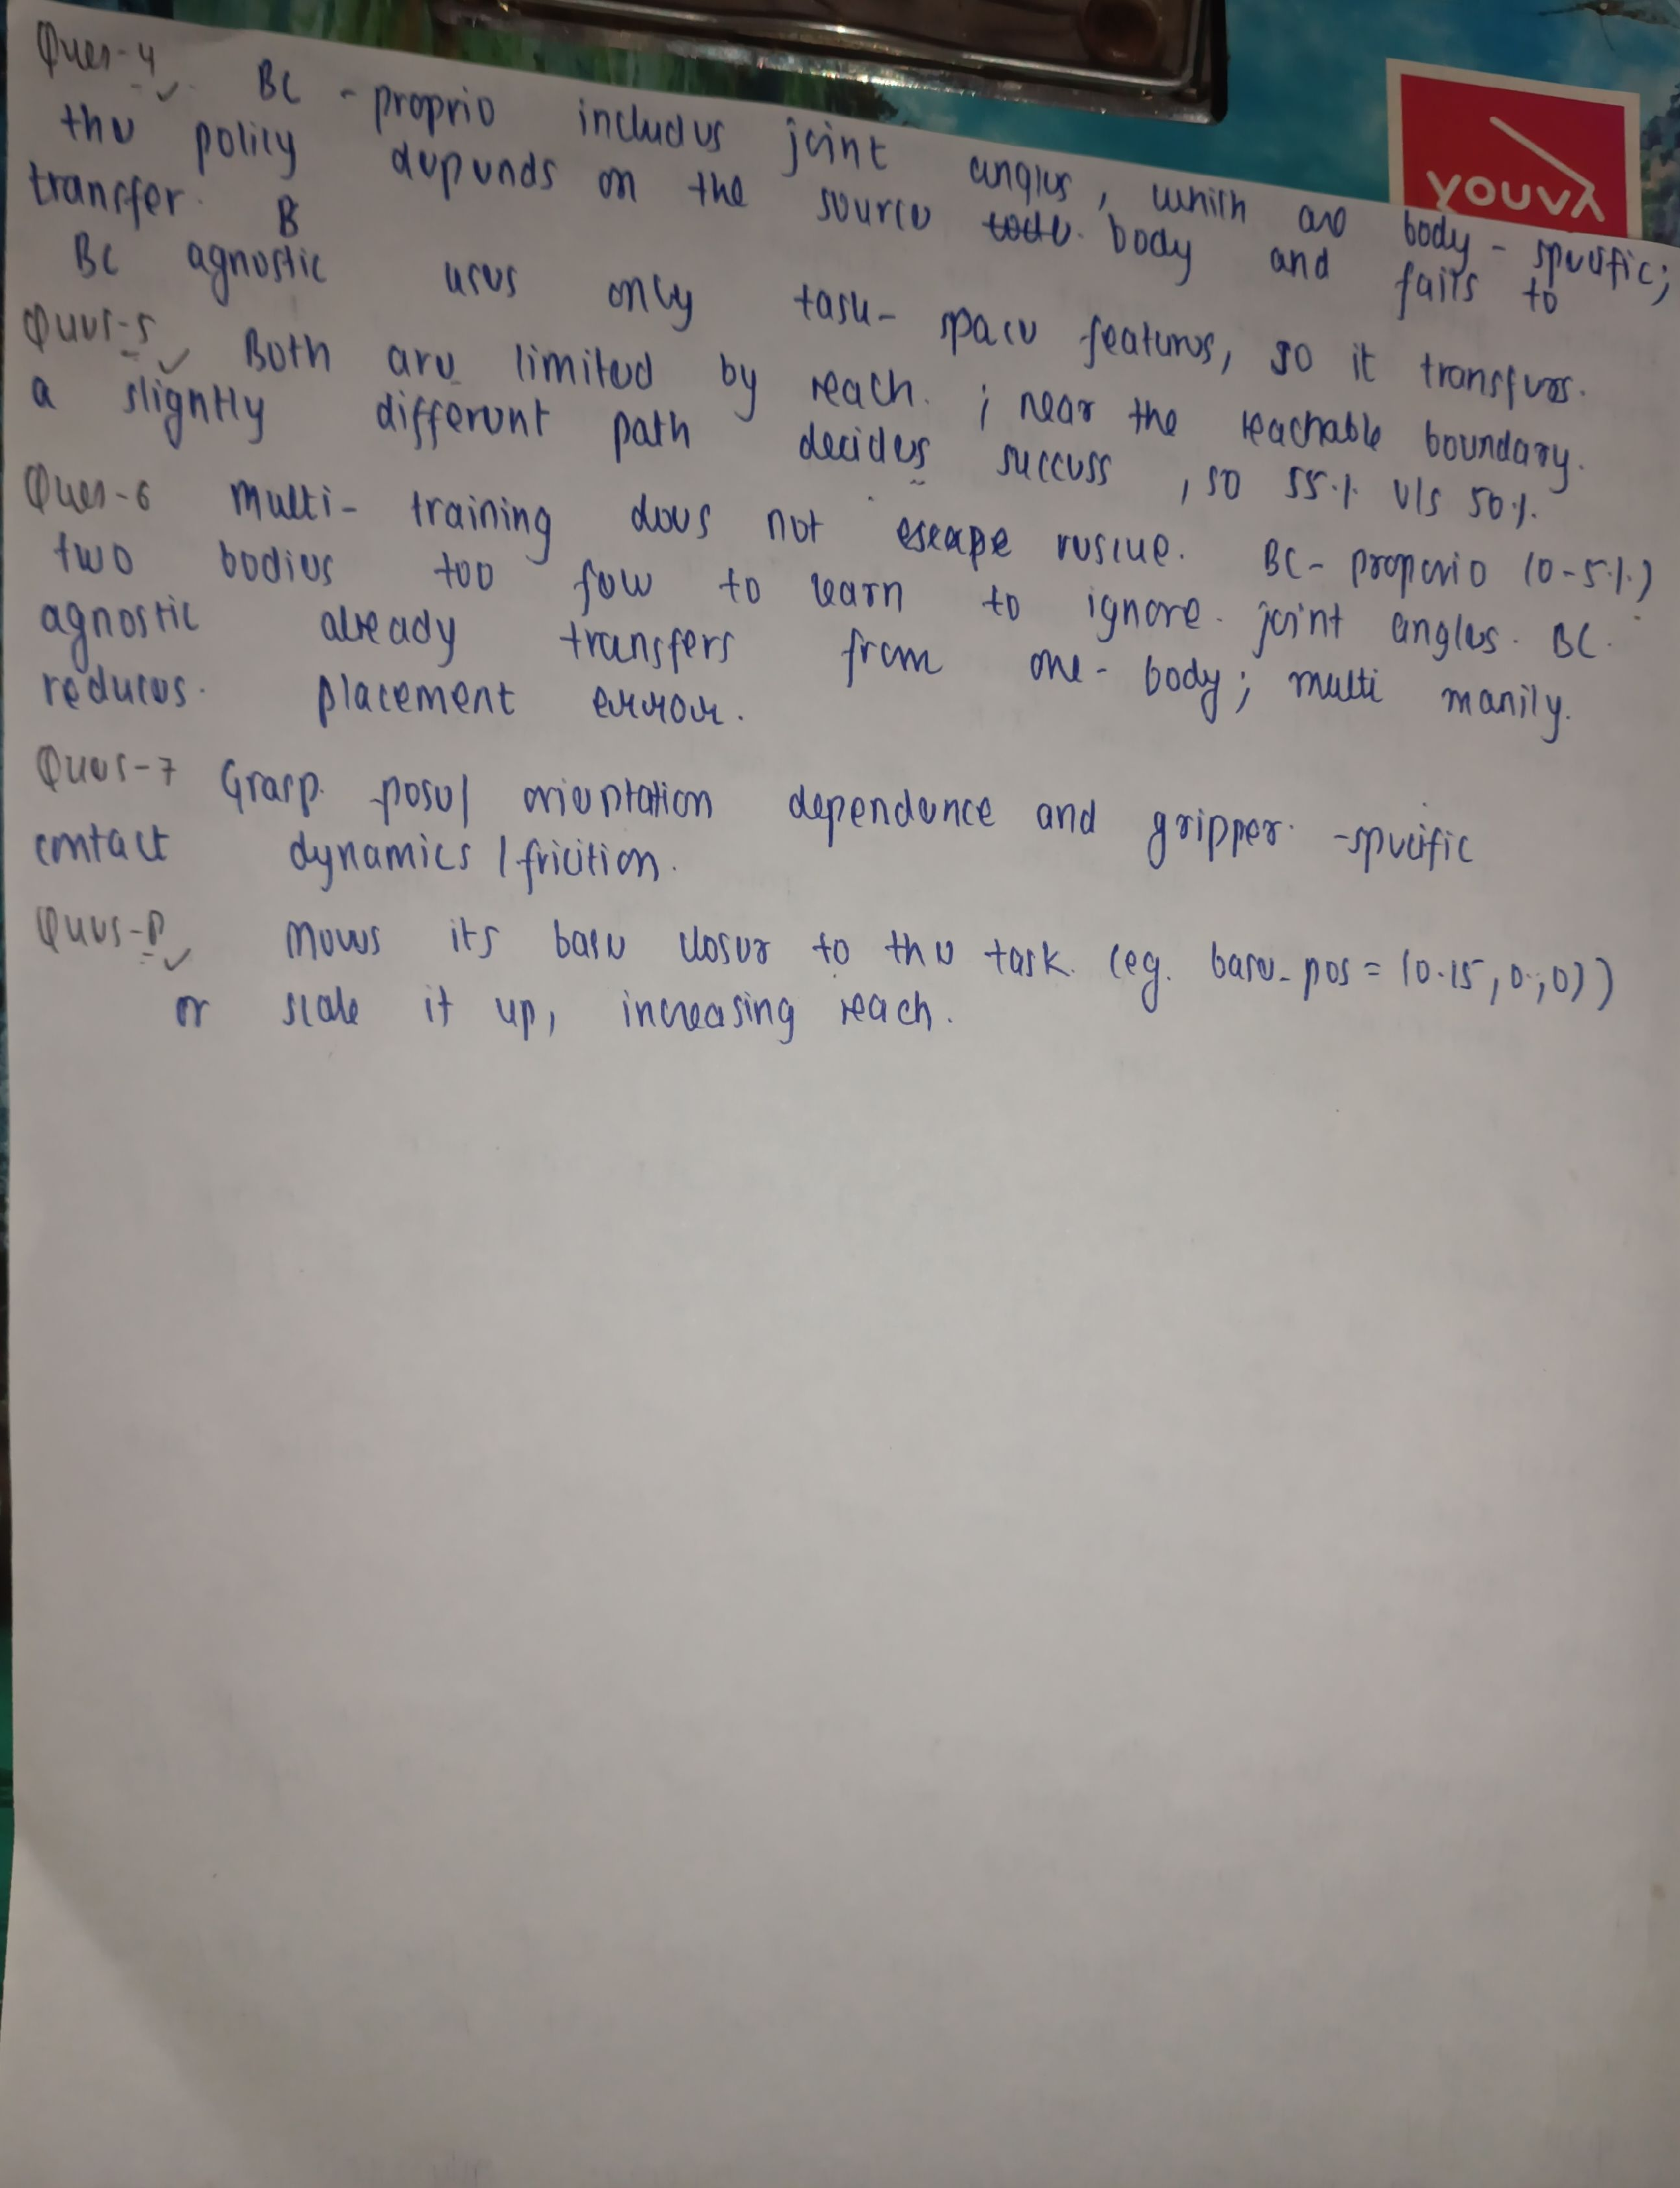
\includegraphics[keepaspectratio,alt={Handwritten answers (scanned) --- page 4}]{handwritten_p4.png}}
\caption{Handwritten answers (scanned) --- page 4}
\end{figure}

\emph{Scanned handwritten answer sheet, page 4, covering this
experiment's Questions section.}

\subsection{8.12 Conclusion}\label{conclusion-7}

A skill in joint space did not transfer even between same-DOF arms.
Task-space interface with per-robot IK let a policy trained on one robot
run on unseen robots. Adding joint angles to observations broke
transfer. No interface can transfer to a body that cannot reach the
task.

\section{Appendix A: GitHub
repository}\label{appendix-a-github-repository}

All code for this report is stored in the GitHub repository:

\texttt{https://github.com/hima-97435/aisr-lab-500121200}

Repository layout:

\begin{verbatim}
aisr-lab-500121200/
  README.md
  report.pdf
  exp01-signals/   exp01.py, figs/
  exp02-queens/    exp02.py, figs/
  exp03-search/    exp03.py, figs/
  exp04-hillclimb/ exp04.py, figs/
  exp05-rl/        exp05.py, figs/
  exp06-neural/    exp06.py, figs/
  exp07-webots/    code/ (webots project), figs/
  exp08-xembody/   code/ (cross-embodiment project), results, models
\end{verbatim}

Commit history documents incremental progress across sessions.

\section{Appendix B: Sources and AI tools
used}\label{appendix-b-sources-and-ai-tools-used}

Sources: - Laboratory Manual, Experiments 1-6, CSAI4014, UPES
(provided). - AISR-Cross-Embodiment-PyBullet manual (MANUAL.md) by
Dr.~Resham Raj Shivwanshi. - Webots robotics simulation guide (GUIDE.md)
and project. - Russell, S. and Norvig, P., Artificial Intelligence: A
Modern Approach, 3rd ed. - Open X-Embodiment Collaboration, ``Open
X-Embodiment'', IEEE ICRA 2024. - Laskey et al., ``DART'', CoRL 2017. -
Coumans, E. and Bai, Y., ``PyBullet'', pybullet.org.

AI tools: - No AI tools were used in the preparation of this report. All
code was written and run by the student.

References (IEEE style):

{[}1{]} S. Russell and P. Norvig, Artificial Intelligence: A Modern
Approach, 3rd ed.~Pearson, 2010.

{[}2{]} E. Coumans and Y. Bai, ``PyBullet, a Python module for physics
simulation,'' pybullet.org, 2016-2024.

{[}3{]} Open X-Embodiment Collaboration, ``Open X-Embodiment: Robotic
Learning Datasets and RT-X Models,'' IEEE ICRA, 2024.

{[}4{]} M. Laskey et al., ``DART: Noise Injection for Robust Imitation
Learning,'' CoRL, 2017.

{[}5{]} V. Braitenberg, Vehicles: Experiments in Synthetic Psychology.
MIT Press, 1984.

{[}6{]} Cyberbotics, ``Webots R2025a,'' cyberbotics.com.

\section{Appendix C: Handwritten answers
(scanned)}\label{appendix-c-handwritten-answers-scanned}

The following pages are the handwritten answer sheets (blue/black ink)
submitted for the Questions sections of all experiments, scanned and
inserted here for reference.

\begin{figure}
\centering
\pandocbounded{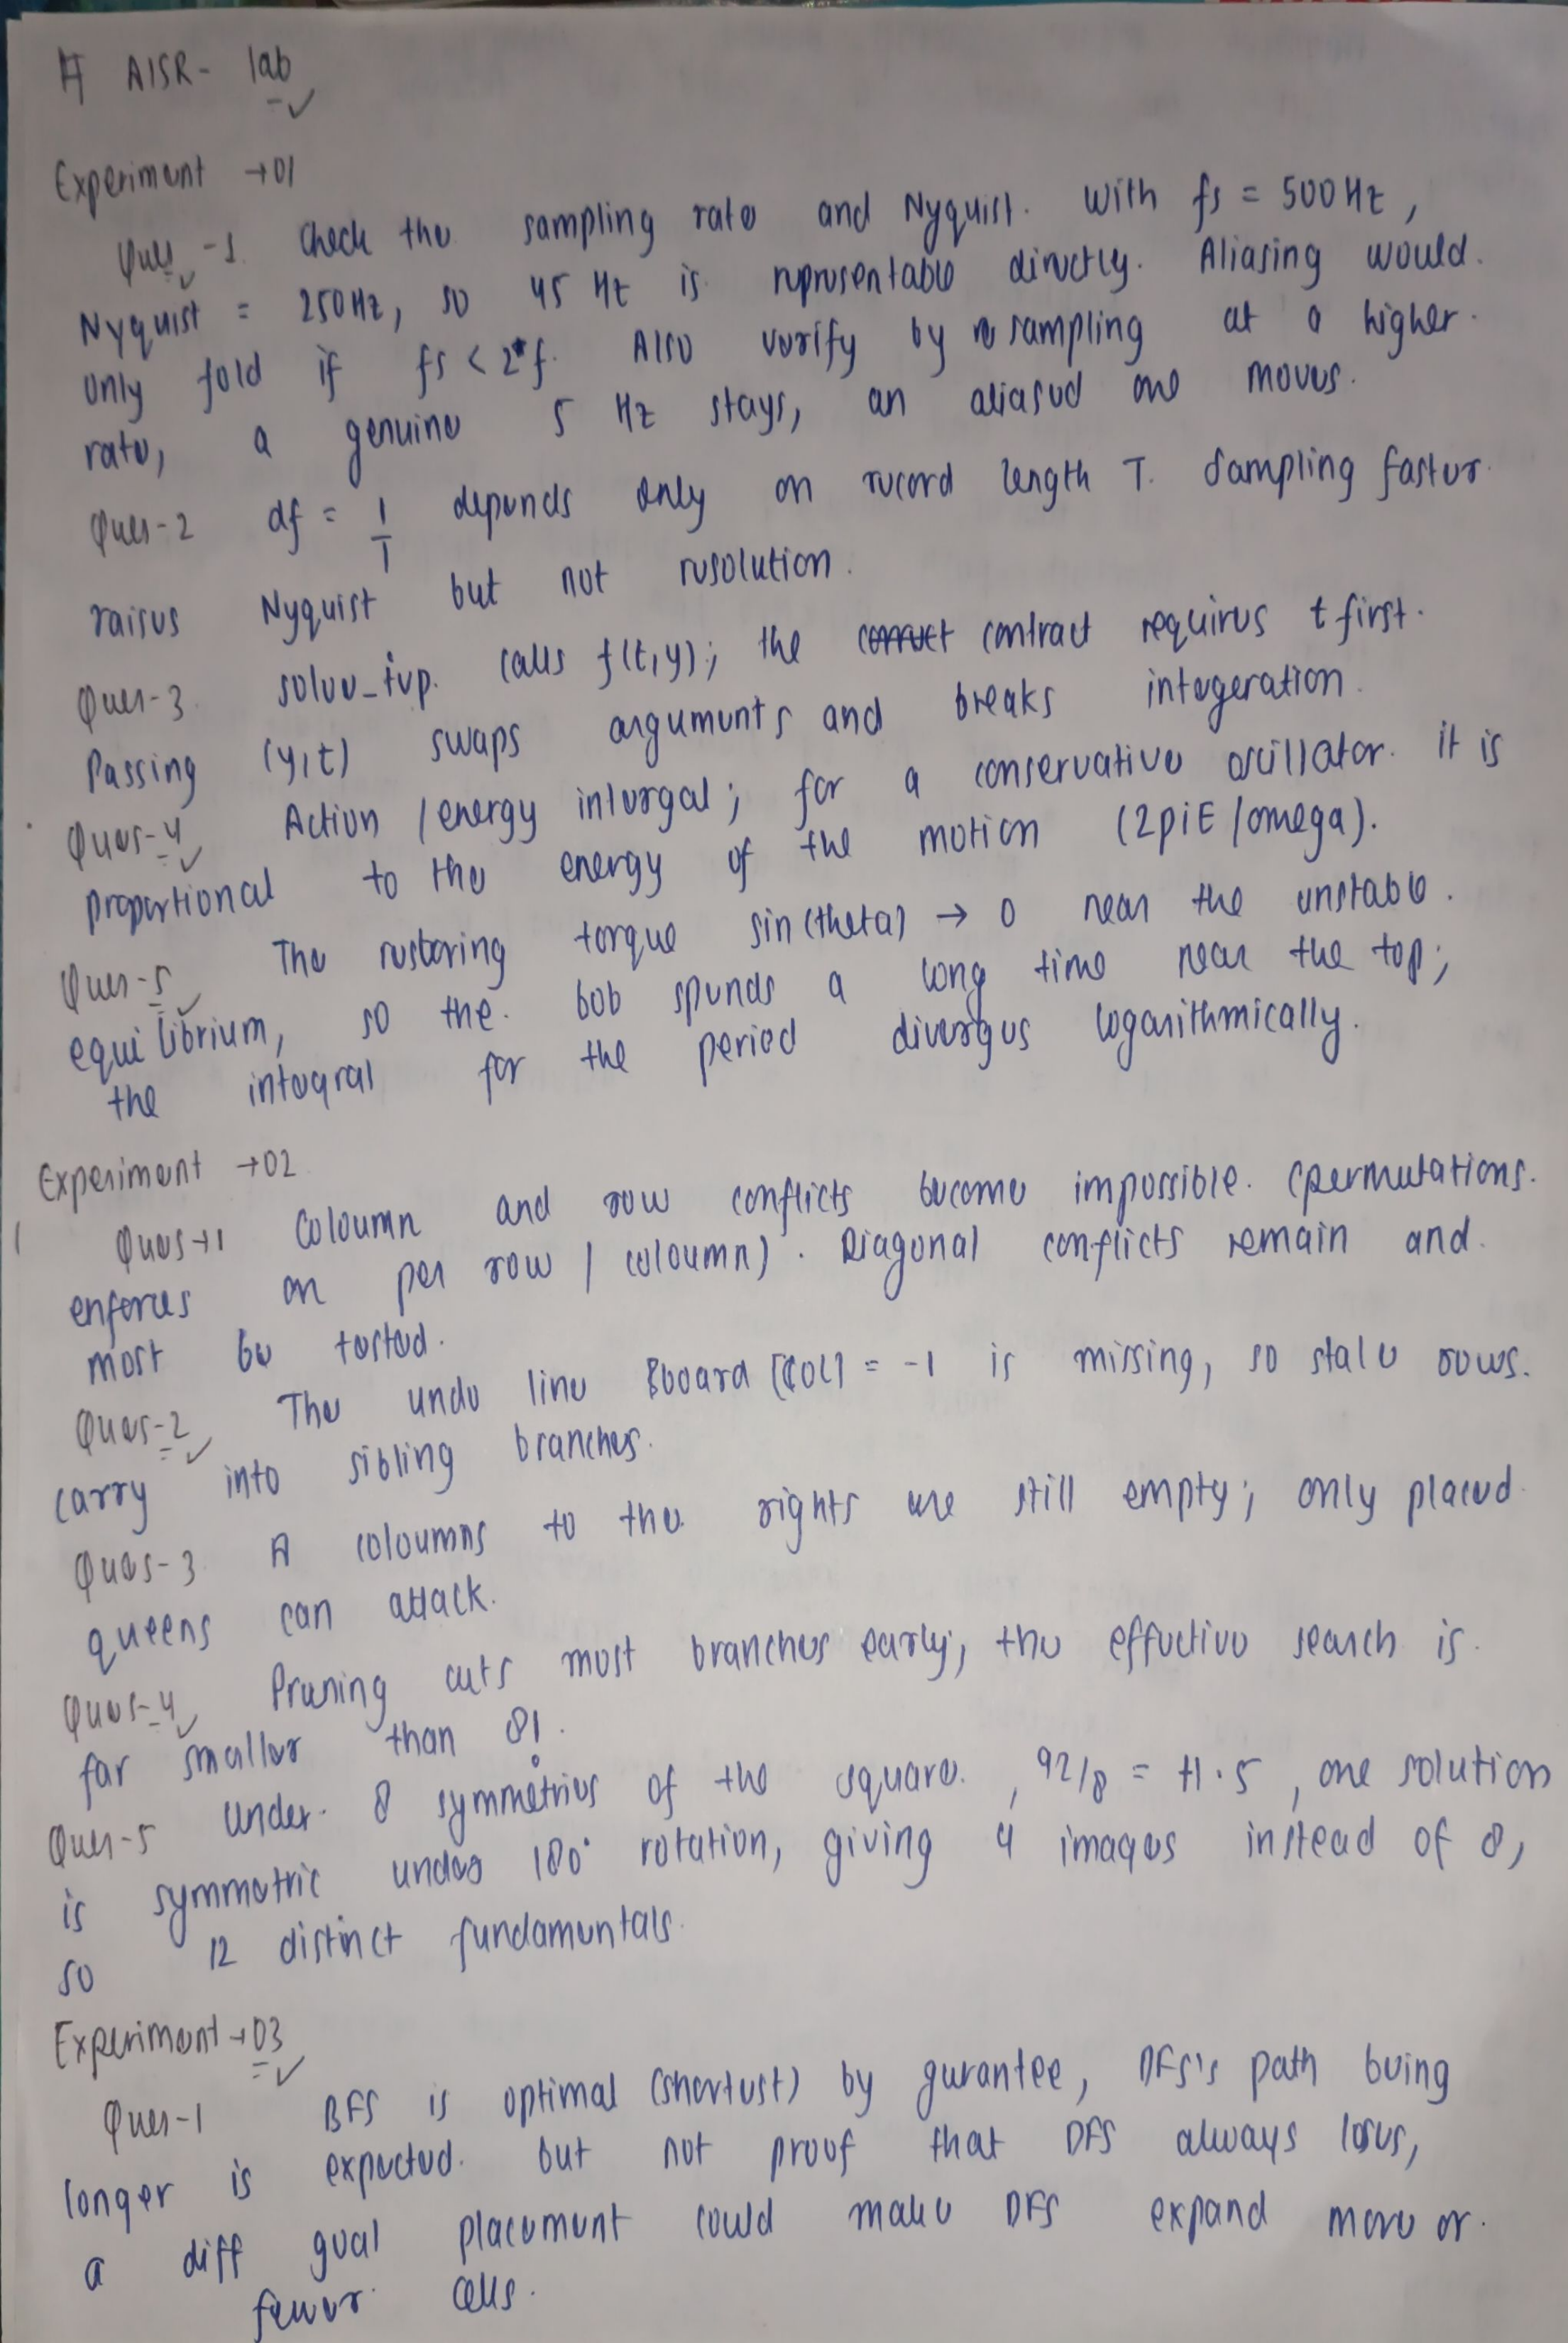
\includegraphics[keepaspectratio,alt={Handwritten answer sheet, page 1}]{handwritten_p1.png}}
\caption{Handwritten answer sheet, page 1}
\end{figure}

\begin{figure}
\centering
\pandocbounded{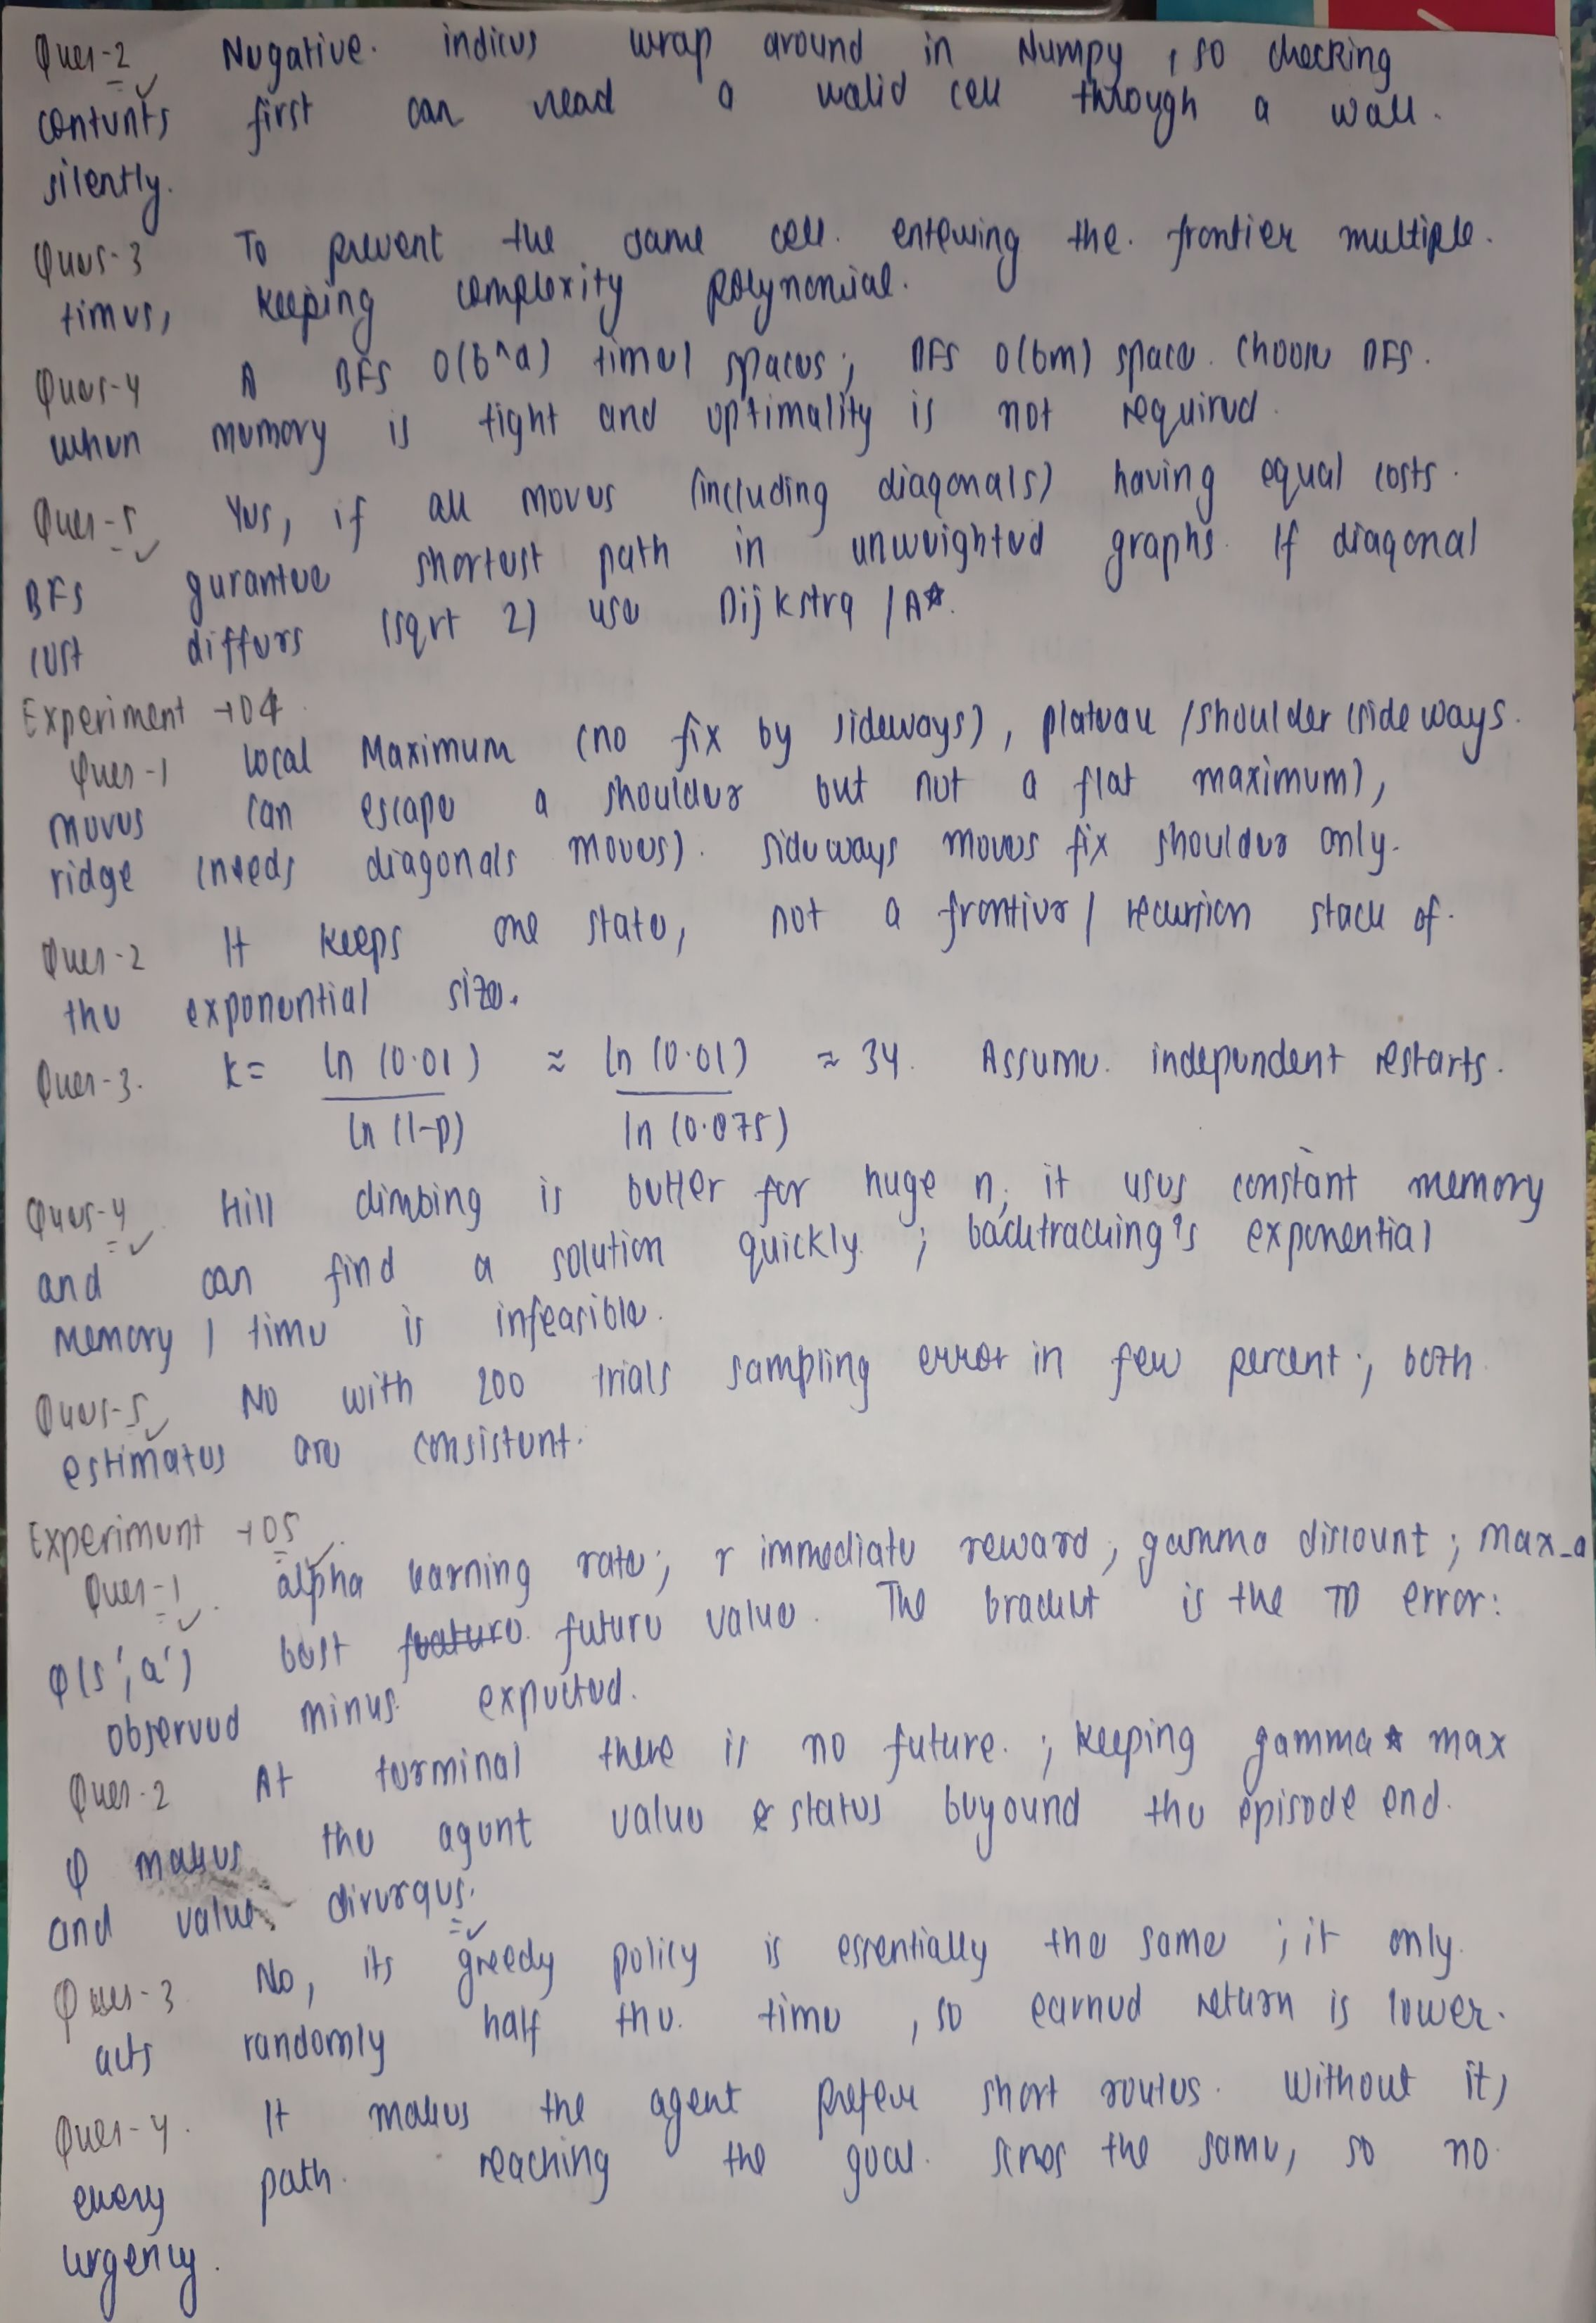
\includegraphics[keepaspectratio,alt={Handwritten answer sheet, page 2}]{handwritten_p2.png}}
\caption{Handwritten answer sheet, page 2}
\end{figure}

\begin{figure}
\centering
\pandocbounded{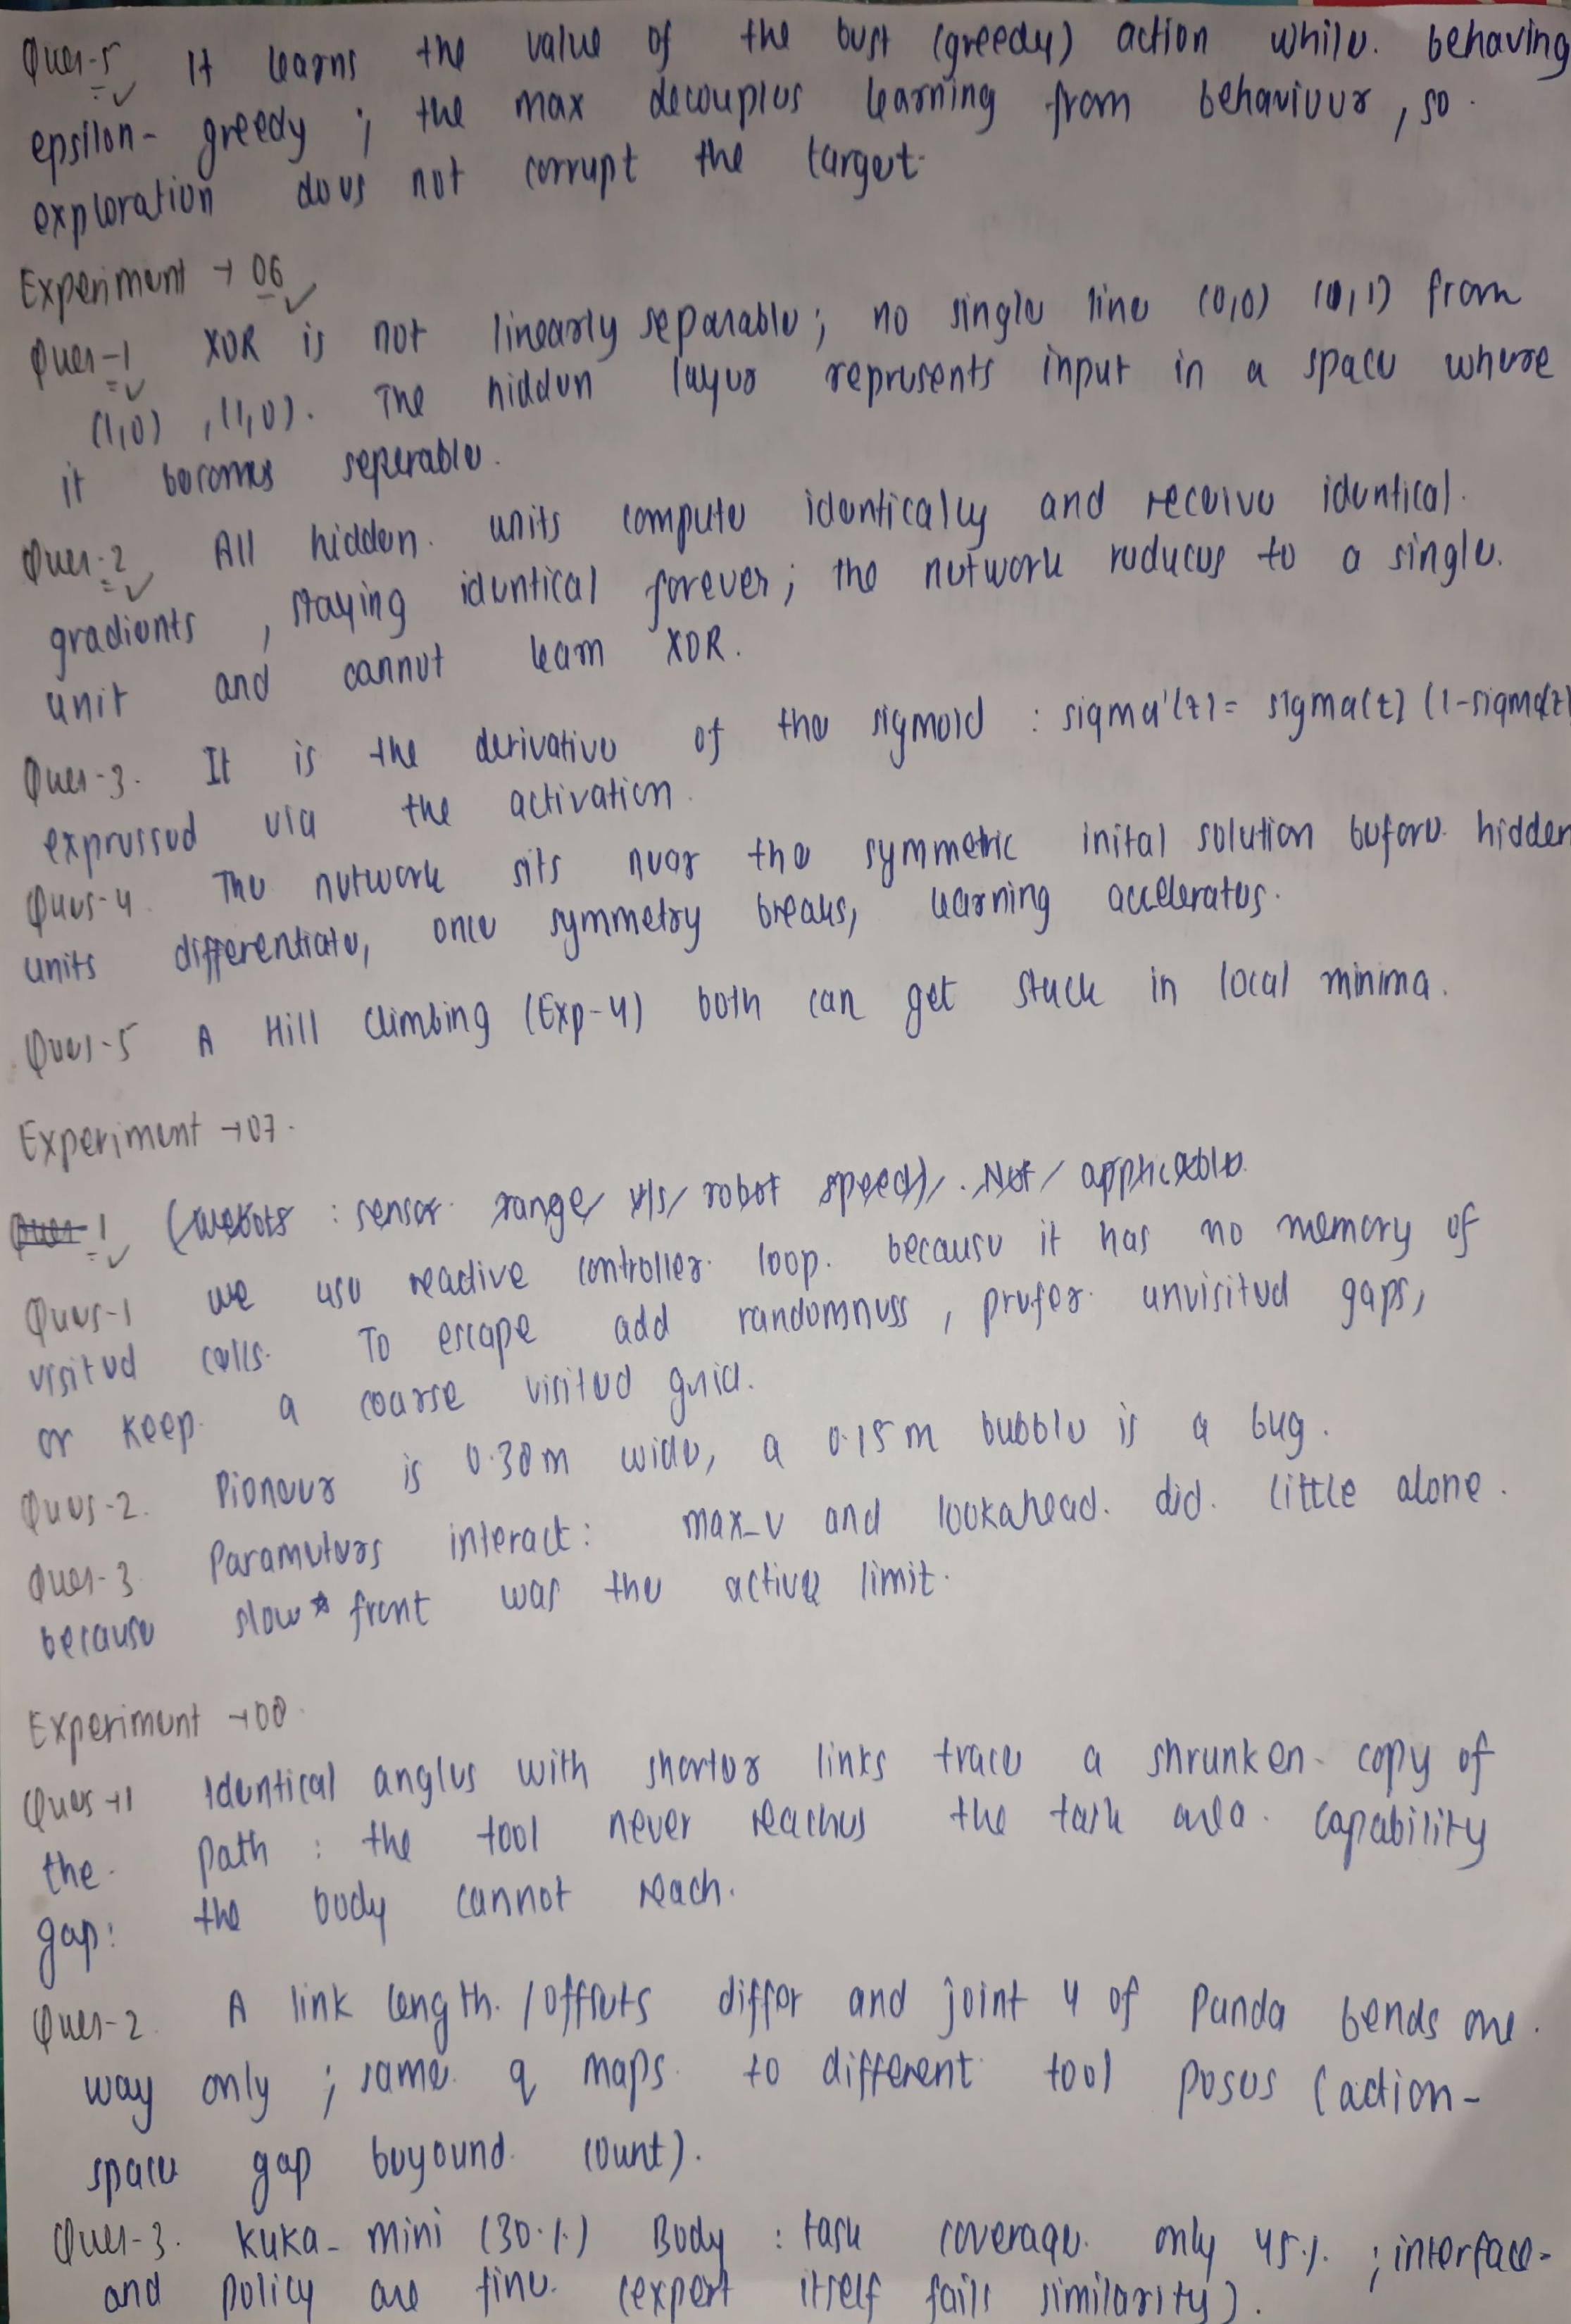
\includegraphics[keepaspectratio,alt={Handwritten answer sheet, page 3}]{handwritten_p3.png}}
\caption{Handwritten answer sheet, page 3}
\end{figure}

\begin{figure}
\centering
\pandocbounded{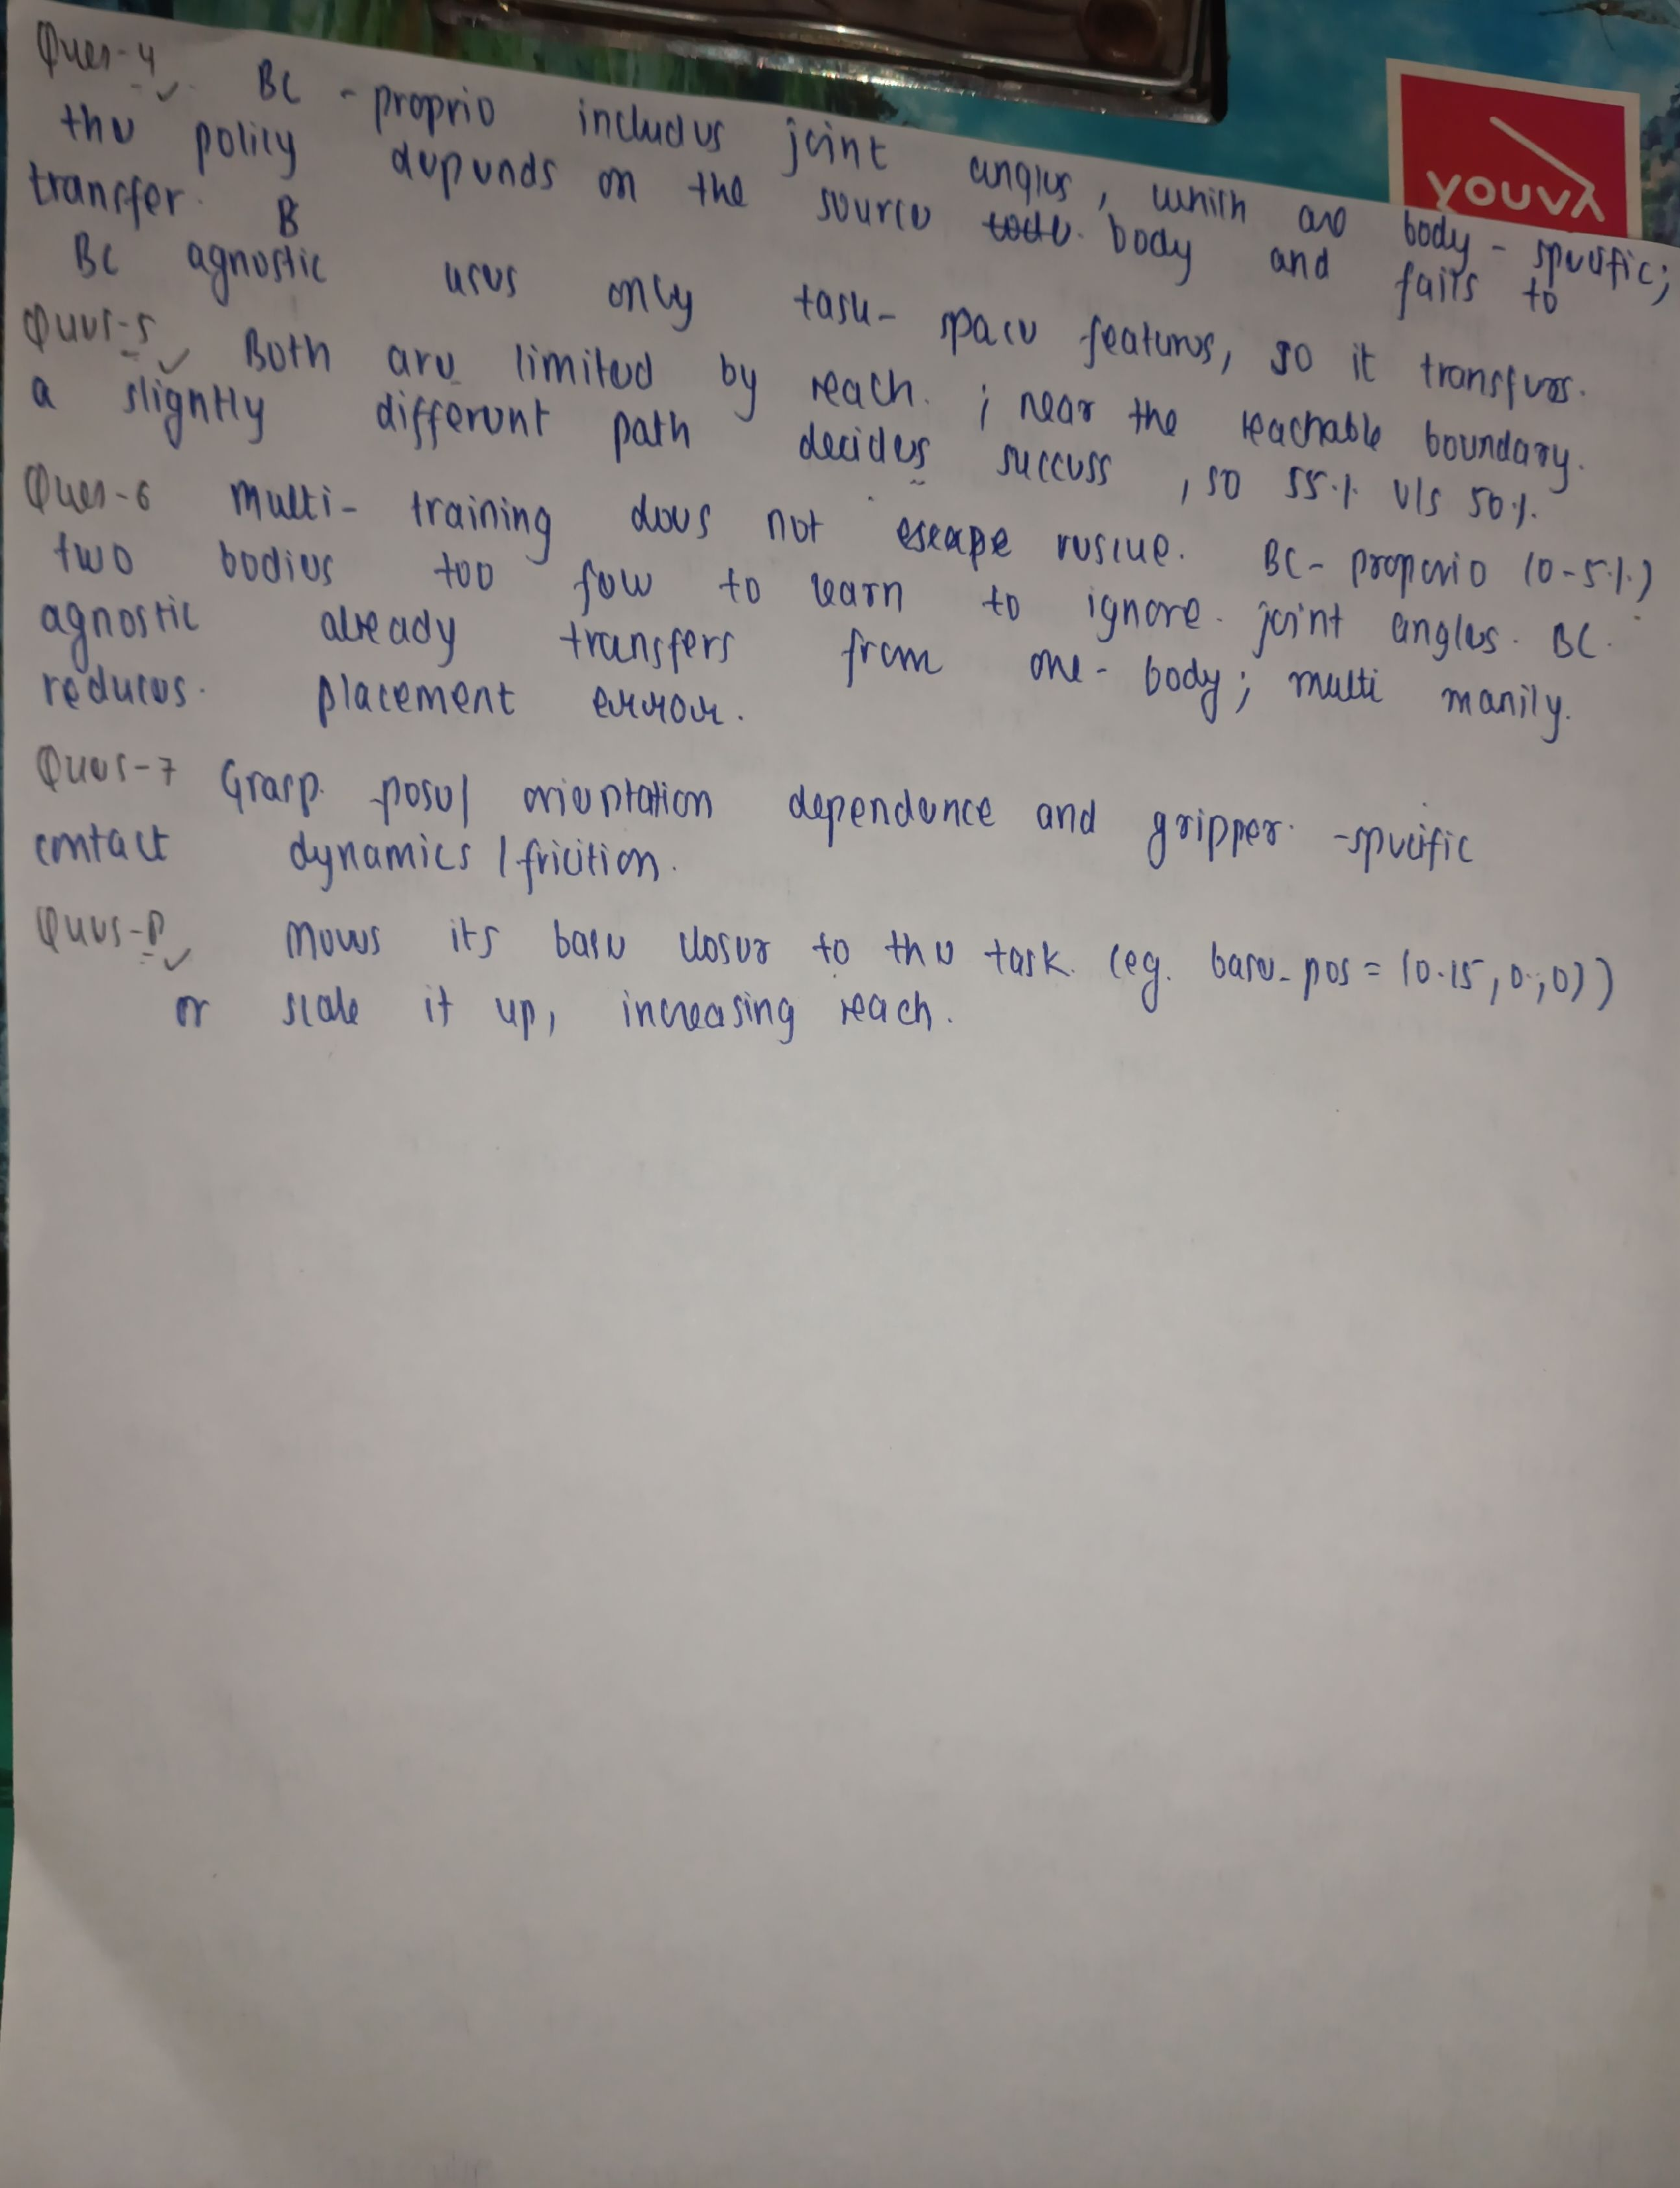
\includegraphics[keepaspectratio,alt={Handwritten answer sheet, page 4}]{handwritten_p4.png}}
\caption{Handwritten answer sheet, page 4}
\end{figure}

\end{document}
